% Gelfand seminar notes, 1975-76: source pages P000603-P000658.
% Russian diplomatic transcription (AI-made, checked against the scans), cut page by page from the cumulative working reader A4-reader-chapters01-34-complete-first1527-separated-diplomatic-r5.
% \SourcePage{GELFAND-Pnnnnnn}{label} starts a scanned page; the second argument is the number written
% on the page, if any. Editorial notes give the page, a label and the transcriber's remark; \Unclear
% marks a doubtful reading.
\SourcePage{GELFAND-P000603}{unlabelled}
\underline{\underline{15.9.75.}}\qquad\underline{Сем. Гельфанда.}

Будет цикл лекций \uwave{Полякова} по физике.

\underline{\underline{Кириллов.}}\qquad\uwave{Теор. J. Vey} о деформации скобки Пуасс.
\Unclear{GELFAND-P000603}{vey-initial}{Инициал читается «J.».}
\end{GelfandAdjacentEvidence}
\begin{GelfandAdjacentEvidence}{GELFAND-P000603}{2}


\((M,\omega)\) — симпл. мн-ие, \([u,v]\) — скобка Пуассона.
Других структур алг. Ли по существу нет (Кириллов и др.). Но если разрешать дифф. опер. пор. \(\infty\), то можно деформ. структуру.

\underline{Теор.:} \(\exists\) формальная деформация скобки Пуассона, ей неэквив.
\[
[u,v]_t=\sum_{k=0}^{\infty}t^k[u,v]^{(k)}
\]
[штрих от \([u,v]^{(k)}\):] опер. пор. \((2k+1)\) по \(u\) и \(v\).

нетривиальность: не свод. заменой координат к исх. скобке Пуасс.
\[
[u,v]^{(k)}=\frac{1}{(2k+1)!}\left(
\frac{\partial^{2k+1}u}{\partial p^{2k+1}}
\frac{\partial^{2k+1}v}{\partial q^{2k+1}}-
\frac{\partial^{2k+1}u}{\partial q^{2k+1}}\cdot
\frac{\partial^{2k+1}v}{\partial p^{2k+1}}\right)+\ldots
\]
\hfill мл. члены\par
На плоскости (или торе) мл. членов нет.
\Unclear{GELFAND-P000603}{lower-terms-abbreviation}{В обоих местах сокращение предположительно читается «мл.».}
\end{GelfandAdjacentEvidence}


Опр. глобально на \(M\) при условии, что \(H^3(M,R)=0\).
\[
?\qquad pq-qp=t
\]


\Needspace{7\baselineskip}
\begin{GelfandAdjacentEvidence}{GELFAND-P000604}{1}
\SourcePage{GELFAND-P000604}{unlabelled}
\underline{\underline{Поляков.}} (\underline{Александр Маркович}).

\underline{Элементарная физика частиц.}

\underline{\(\gamma\) — фотон.} — отдельн. группа

\underline{Лептоны}
\[
\begin{array}{@{}l@{}}
\begin{array}{@{}ll@{}}
e^- & m=0{,}5\\
\mu^- & m=105
\end{array}\\[-.1ex]
\left.\begin{array}{@{}ll@{}}
\nu_e & m=0\\
\nu_\mu & m=0
\end{array}\right\}\text{ нейтрино}
\end{array}
\]
\par\noindent\rule{.31\linewidth}{.45pt}\par

\underline{Адроны.}
\[
\begin{array}{ll}
p & m=940\\
n & \text{— \(\Vert\) —}\\
\pi & m=140
\end{array}
\]
и др.
\par\noindent\rule{.31\linewidth}{.45pt}\par
\Unclear{GELFAND-P000604}{pion-mark}{Верхний штрих в записи \(\pi\) отделён от нижних.}
\end{GelfandAdjacentEvidence}
\begin{GelfandAdjacentEvidence}{GELFAND-P000604}{2}


\underline{Взаимодействия:}\qquad
\dashuline{Интенсивность в единицах} \(x=\dfrac{E_{\text{вз}}}{m}\)
\[
\begin{array}{lll}
\mathrm{Gr} & (\text{гравит.}) & x\sim10^{-38}\\
\mathrm W & (\text{слабое}) & x\sim10^{-5}\\
\mathrm{EM} & (\text{эл.-магн.}) & x\sim10^{-2}\\
\mathrm S & (\text{сильное}) & x\sim1
\end{array}
\]
Чем слабее взаимод., тем оно более лояльно (нарушает меньше законов сохранения).

Отличают их только благодаря симметрии (сильное от слабого — т.к. оба [зачёркнуто] близкодействующие).
\Incomplete{GELFAND-P000604}{cancel-after-oba}{Слово после «оба» густо зачёркнуто.}
\end{GelfandAdjacentEvidence}
\begin{GelfandAdjacentEvidence}{GELFAND-P000604}{3}


\underline{Лептоны} — все взаим., кроме сильного.

\underline{Адроны} — все 4 взаимод..

\uwave{Квантовая электродинамика} описывает эл.-магн. взаимод. лептонов. (остальные слабее и пока игнорируются).

Частица описывается своим полем. Нужно указ. действие:
\[
S=S[e(x),\mu(x),\ldots]
\]
Инвариантность: вращ., трансл., преобр. Лоренца.

\dashuline{Экспер. факт}: электрон при вращ. преобр. по спинорному представлению
\[
\begin{pmatrix}e'_1\\e'_2\end{pmatrix}
=\exp\left(\frac i2(\bar\sigma\,\bar\Theta)\right)
\begin{pmatrix}e_1\\e_2\end{pmatrix}
\]
\hfill(\(e_j\in\mathbb C\) — компоненты спинора)\par

\(\bar\sigma\) [зачёркнуто] — матрицы Паули (набор 3-х таких матриц); \(\bar\Theta\in\mathbb R^3\);
\Unclear{GELFAND-P000604}{cancel-after-sigma}{Запись после \(\bar\sigma\) густо зачёркнута.}
\end{GelfandAdjacentEvidence}


\(|\bar\Theta|\) — угол вращ., напр. \(\Theta\) — напр. оси вращения.


\Needspace{7\baselineskip}
\begin{GelfandAdjacentEvidence}{GELFAND-P000605}{1}
\SourcePage{GELFAND-P000605}{unlabelled}
\[
\sigma_x=\begin{pmatrix}0&1\\1&0\end{pmatrix},\quad
\sigma_y=\begin{pmatrix}0&-i\\i&0\end{pmatrix},\quad
\sigma_z=\begin{pmatrix}1&0\\0&-1\end{pmatrix}.
\]
\Unclear{GELFAND-P000605}{matrix-upper-entry}{Перед верхней правой единицей в \(\sigma_x\) виден короткий штрих, возможно минус.}
\end{GelfandAdjacentEvidence}
\begin{GelfandAdjacentEvidence}{GELFAND-P000605}{2}

Вычис. и преобр. при действии группы Лоренца. 2 возможности:
\Unclear{GELFAND-P000605}{initial-verb}{Начальное сокращение предположительно читается «Вычис.».}
\end{GelfandAdjacentEvidence}
\begin{GelfandAdjacentEvidence}{GELFAND-P000605}{3}

\[
e'_L=\exp\left(\frac{\bar\sigma\bar\psi}{2}\right)e_L,
\]
где \(\bar\psi\) — вектор, коллинеарный вект. скорости:
\[
v=\operatorname{th}|\bar\psi|,\qquad
\frac{\vec v}{|\bar v|}=\frac{\bar\psi}{|\bar\psi|}
\qquad(\bar\psi\text{ — тоже 3-вектор})
\]
[под строкой] «быстрота»
\[
e'_R=\exp\left(-\frac{\bar\sigma\bar\psi}{2}\right)e_R
\]
\rule{.21\linewidth}{.4pt}\par
\underline{Поясн.} (Г.) [зачёркнуто]. \(SO(3)\longrightarrow\)
[зачёркнуто]. \(SU(2)\).
\Incomplete{GELFAND-P000605}{cancel-before-so}{Перед \(SO(3)\) зачёркнута запись.}
\end{GelfandAdjacentEvidence}
\begin{GelfandAdjacentEvidence}{GELFAND-P000605}{4}

\Incomplete{GELFAND-P000605}{cancel-before-su}{Перед \(SU(2)\) зачёркнута запись.}
\end{GelfandAdjacentEvidence}
\begin{GelfandAdjacentEvidence}{GELFAND-P000605}{5}

\Unclear{GELFAND-P000605}{so-su-direction}{Стрелка на листе направлена от \(SO(3)\) к \(SU(2)\).}
\end{GelfandAdjacentEvidence}
\begin{GelfandAdjacentEvidence}{GELFAND-P000605}{6}

\[
\bar\Theta\text{ — вращ. в }\mathbb R^3\Longrightarrow\text{матр.}\in SU(2)
\]
(представление \(SU(2)\))

Это предст. прод. до предст. группы Лоренца.

Преобр. Лор. — вектор скорости \(\vec v\) (вращение опускается)
(собств. преобр. Лоренца)

\uwave{Быстрота} \(\bar\psi\) — ввод. вместо \(\bar v\)

\rule{.28\linewidth}{.4pt}\par
\underline{\underline{П.}}
\[
\left\{\begin{aligned}
t'&=t\operatorname{ch}\psi+z\operatorname{sh}\psi\\
z'&=z\operatorname{ch}\psi+t\operatorname{sh}\psi
\end{aligned}\right.
\]
\Unclear{GELFAND-P000605}{boost-z-overwrite}{В первой строке \(z\) написано поверх прежнего знака.}
\end{GelfandAdjacentEvidence}
\begin{GelfandAdjacentEvidence}{GELFAND-P000605}{7}

[справа] — запись пр. Лоренца через \(\psi\).
(собств. преобр. Лоренца — без добавки вращ. и переноса).

Электрон либо \(e_L\) либо \(e_R\).

Но есть симметрия \(\vec x\longrightarrow-\vec x\), \(\vec v\longrightarrow-\vec v\), они перех. друг в друга.

Если присоед. отражение, то предст. получается лишь комбинир.:
\[
\hat p\begin{pmatrix}e_L\\e_R\end{pmatrix}
=\begin{pmatrix}e_R\\e_L\end{pmatrix}.
\]
Надо вв. \underline{биспинор}: \(\begin{pmatrix}e_L\\e_R\end{pmatrix}\).

Тогда плотн. лагранжиана:
\[
\begin{aligned}
\mathcal L'&=e_L^+(x)\left\{\frac{\partial}{\partial t}
-\left(\bar\sigma\frac{\partial}{\partial\bar x}\right)\right\}e_L(x)\\
&\quad+e_R^+(x)\left\{\frac{\partial}{\partial t}
+\left(\bar\sigma\frac{\partial}{\partial\bar x}\right)\right\}e_R(x)
\end{aligned}
\]
\((z^+=\bar z)\).

Действие: \(S=\int\mathcal L\,dt\,d^3\bar x\).
\Unclear{GELFAND-P000605}{action-prime}{В формуле действия у \(\mathcal L\) штрих не виден.}
\end{GelfandAdjacentEvidence}


Легко пров. инвариантность.

\underline{Безмассовость}\qquad Ур-е Лагр.
\[
\left(\frac{\partial}{\partial t}-\bar\sigma\frac{\partial}{\partial\bar x}\right)e_L=0
\]
Сделаем пр. Фурье: \((E-\bar\sigma\bar p)e_L=0\) и след. \(E^2=p^2\).


\Needspace{7\baselineskip}
\begin{GelfandAdjacentEvidence}{GELFAND-P000606}{1}
\SourcePage{GELFAND-P000606}{unlabelled}
Отсюда \(E\) сколь угодно мало (при малом \(p\)) \(\Rightarrow m=0\).

Надо доб. член с массой. Инвар. способ единственен

\sout{\(e_L\)} [зачёркнуто] \sout{\(me\)}
\Unclear{GELFAND-P000606}{canceled-mass-connector}{Под зачёркиванием между \(e_L\) и \(me\) виден знак, похожий на стрелку вправо.}
\end{GelfandAdjacentEvidence}
\begin{GelfandAdjacentEvidence}{GELFAND-P000606}{2}

\begin{center}
\uwave{\(m(e_L^+e_R+e_R^+e_L)\)}.
\end{center}
Итак: окончательный вид лагранжиана:
\[
\mathcal L=\mathcal L'+m(e_L^+e_R+e_R^+e_L).
\]
\underline{\underline{Эквив. вид}}: пусть \(e=\begin{pmatrix}e_L\\e_R\end{pmatrix}\). (биспинор).
\[
\mathcal L=\bar e\left(i\gamma_\mu\frac{\partial}{\partial x_\mu}-m\right)e
\]
\[
\gamma_\mu\frac{\partial}{\partial x_\mu}
=\gamma_0\frac{\partial}{\partial t}-\bar\gamma\frac{\partial}{\partial\bar x},
\qquad \bar e=e^+\gamma_0
\]
\(\gamma_\mu\) — матр. Дирака,
\(\gamma_\mu\gamma_\nu+\gamma_\nu\gamma_\mu=2g_{\mu\nu}\),
\[
g_{\mu\nu}=\begin{pmatrix}
1&&&0\\
&-1&&\\
&&-1&\\
0&&&-1
\end{pmatrix}\text{ — метр. Минковского.}
\]
\(\gamma_\mu\) выписываются через матрицы \(\sigma\)

(\underline{Лит-ра}: Ландау, Берестецкий, Лифшиц, Питаевский — Релятивистская квант. теория, ч. 1).

\dashuline{Спектр}: \(E=\sqrt{p^2+m^2}\).

(В ур-и Дирака \(\left(i\gamma_\mu\dfrac{\partial}{\partial x_\mu}-m\right)e=0\)
переходим к Фурье-преобр. получ. этот рез.)
\[
\rule{1.8em}{.4pt}\;\boldsymbol{\cdot}\;\rule{1.8em}{.4pt}
\]
\dashuline{Калибров. группа}\qquad \(e'\Rightarrow e^{i\beta}e\). \((\beta\in\mathbb R)\).
\Unclear{GELFAND-P000606}{gauge-arrow}{Две горизонтальные линии между \(e\prime\) и \(e^{i\beta}e\), у верхней виден наконечник вправо.}
\end{GelfandAdjacentEvidence}
\begin{GelfandAdjacentEvidence}{GELFAND-P000606}{3}


\(\mathcal L\) инвариантно и относит. этой группы\qquad \uwave{\(e'=(2{,}7\ldots)^{i\beta}e\)}

\dashuline{Гипотеза}: меняем фазу по разному в разных точках и треб. ковар. относит. этих преобразований (предельная локальность)
\[
\underline{e'=(2{,}7)^{i\beta(x)}e}
\]
\uwave{Инвар. уже нет}:
\[
\bar e\left(i\gamma_\mu\left(\frac{\partial}{\partial x_\mu}+i\partial_\mu\beta\right)-m\right)e.
\]
\[
\mathcal L'=\bar e\biggl(i\gamma_\mu\frac{\partial}{\partial x_\mu}
+iA_\mu(x)\biggr)-m\biggr)e
\]
\Unclear{GELFAND-P000606}{a-term-contraction}{После \(A_\mu(x)\) и после \(-m\) стоят закрывающие скобки. Перед \(iA_\mu(x)\) не видно множителя \(\gamma_\mu\).}
\end{GelfandAdjacentEvidence}



\Needspace{7\baselineskip}
\begin{GelfandAdjacentEvidence}{GELFAND-P000607}{1}
\SourcePage{GELFAND-P000607}{unlabelled}
(\(A_\mu(x)\) — связность).
\[
\begin{gathered}
A'_\mu(x)=A_\mu-\partial_\mu\beta.\\
\nabla_\mu=\partial_\mu+iA_\mu.
\end{gathered}
\]
Если это сделать, то общ. ковариантность восстановится.
\Unclear{GELFAND-P000607}{covariance-abbreviation}{Перед «ковариантность» сокращение читается «общ.».}
\end{GelfandAdjacentEvidence}
\begin{GelfandAdjacentEvidence}{GELFAND-P000607}{2}


Из \(\mathcal L'\) не возникают ур-я для \(A_\mu\). Нужна кривизна
\[
F_{\mu\nu}=\partial_\mu A_\nu-\partial_\nu A_\mu
\]
Это тензор, а в [зачёркнуто] \(\mathcal L\) ввод. квадрат.
\Unclear{GELFAND-P000607}{cancel-before-l}{Перед \(\mathcal L\) зачёркнута запись.}
\end{GelfandAdjacentEvidence}
\begin{GelfandAdjacentEvidence}{GELFAND-P000607}{3}

\[
\mathcal L=\text{[зачёркнуто]}\ \mathcal L'+\left(\frac1{4e^2}\right)F_{\mu\nu}^2
\]
\Unclear{GELFAND-P000607}{cancel-coefficient}{Перед \(\mathcal L\prime\) в правой части зачёркнут знак.}
\end{GelfandAdjacentEvidence}
\begin{GelfandAdjacentEvidence}{GELFAND-P000607}{4}

(\(e\) — заряд электрона)
\[
\rule{1.8em}{.4pt}\;\boldsymbol{\cdot}\;\rule{1.8em}{.4pt}
\]
\underline{Рассеяние.}\qquad \(S=S[\varphi(x)]\).
\[
B\qquad \varphi_{\mathrm{in}}(x)\longrightarrow\varphi_{\mathrm{out}}(x)
\]
\Unclear{GELFAND-P000607}{scattering-margin}{Слева от стрелочной записи отдельный знак, похожий на «В» с вертикальным штрихом.}
\end{GelfandAdjacentEvidence}
\begin{GelfandAdjacentEvidence}{GELFAND-P000607}{5}

\[
\varphi_{\mathrm{in}}(x)=\lim_{t\to-\infty}\varphi(\bar x,t),\qquad
\varphi_{\mathrm{out}}(x)=\lim_{t\to+\infty}\varphi(\bar x,t).
\]
\[
\int_{\Phi_{\mathrm{in}}}^{\Phi_{\mathrm{out}}}D\varphi(x)\,e^{iS[\varphi]}
=M\text{ — амплитуда перехода}
\]
(функц. интегрирование, \(D\varphi\) — естеств. мера, [под строкой] (лебеговская),
интеграл по всем \(\Phi(x,t)\),
\(\Phi(x,+\infty)=\Phi_{\mathrm{out}}\),
\(\varphi(x,-\infty)=\varphi_{\mathrm{in}}\))

Есть правила вычисления.

[зачёркнуто] [вставлено сверху в обводке] Без \(A_\mu\) — гауссов интеграл (Френеля)
\Incomplete{GELFAND-P000607}{cancel-gaussian}{Перед вставкой и словами «гауссов интеграл» запись густо зачёркнута.}
\end{GelfandAdjacentEvidence}
\begin{GelfandAdjacentEvidence}{GELFAND-P000607}{6}


Потом — теория возмущений (счит. \(A_\mu\) малым); \(eA_\mu e\) — кубич. член

\rule{.22\linewidth}{.4pt}\par
\underline{Г.}\qquad \(\int e^{i(x^2+\varepsilon x^3)}\,dx\) — ваша теория

Важно:
\[
\int e^{-\sum a_{ik}x_ix_k+\varepsilon\sum x_i^3}\,dx
\]
\[
\int e^{ix^2(1+\varepsilon x^3)}=\sum c_k\int x^k e^{ix^2}\,dx
\]
\Unclear{GELFAND-P000607}{x-power-discrepancy}{В показателе написано \(ix^2(1+\varepsilon x^3)\).}
\end{GelfandAdjacentEvidence}
\begin{GelfandAdjacentEvidence}{GELFAND-P000607}{7}


Для этого прим. диагр. Фейнмана.

[зачёркнуто слева] \(\int\frac{\phantom{dx}}{(x^2+y^2+z^2+t\ldots)}\)
\Incomplete{GELFAND-P000607}{cancel-integral}{В зачёркнутой записи различимы знак интеграла, дробная черта и часть знаменателя.}
\end{GelfandAdjacentEvidence}
\begin{GelfandAdjacentEvidence}{GELFAND-P000607}{8}


Напр.
\[
\int\frac{dx\,dy\,dz\,dt}
{(x^2+y^2+z^2+t^2+m_1)(x^2+y^2+z^2+t^2+m_2)}
\]
\Unclear{GELFAND-P000607}{denominator-deletion}{После первого \(t^2\) зачёркнута скобка. Во втором множителе показатель у \(y\) переписан.}
\end{GelfandAdjacentEvidence}

(украдено Ф. у Швингера)
\[
\frac1{ab}=\int_0^1\frac{ds}{(sa+(1-s)b)^2}.\qquad
\frac1{abc}\text{ аналогично.}
\]


\Needspace{7\baselineskip}
\begin{GelfandAdjacentEvidence}{GELFAND-P000608}{1}
\SourcePage{GELFAND-P000608}{unlabelled}
\underline{П.} можно ещё \(\dfrac1{a^\lambda b^\mu c^\gamma}\)
\Unclear{GELFAND-P000608}{triple-exponent}{Показатель при \(a\) переписан, предположительно \(\lambda\).}
\end{GelfandAdjacentEvidence}
\begin{GelfandAdjacentEvidence}{GELFAND-P000608}{2}

\[
\frac1{a^\lambda b^\mu}
=\int_0^1\frac{s^{\lambda-1}(1-s)^{\mu-1}}{(sa+(1-s)b)^{\lambda+\mu}}\,ds
\]
\[
\frac1{\prod a_i^{\lambda_i}}
=\int_{s_i\geq0.}\frac{\prod ds_i\,\delta(\sum s_i-1)\,s_i^{\lambda_i-1}}
{(\sum s_i a_i)^{\sum\lambda_j}}
\]
\Unclear{GELFAND-P000608}{parameter-normalization}{Обе формулы записаны без отдельного нормировочного множителя.}
\end{GelfandAdjacentEvidence}
\begin{GelfandAdjacentEvidence}{GELFAND-P000608}{3}

\[
\rule{1.8em}{.4pt}\;\boldsymbol{\cdot}\;\rule{1.8em}{.4pt}
\]
Считаем по \dashuline{теории возмущений}:

\(x,\ x'\)

\uwave{Амплитуда перех. из \(x\) в \(x'\)}: \(K(x,x')\) по Максвеллу
\[
\left(i\gamma_\mu\frac{\partial}{\partial x_\mu}-m\right)K(x,x')=\delta(x-x').
\]
\Unclear{GELFAND-P000608}{kernel-gamma-writing}{Знак \(\gamma\) утолщён и, возможно, переписан.}
\end{GelfandAdjacentEvidence}
\begin{GelfandAdjacentEvidence}{GELFAND-P000608}{4}

\SourceFigure{GELFAND-P000608}{photon-exchange}{%
\par\smallskip
\begingroup\color{black}\GelfandFitDiagram{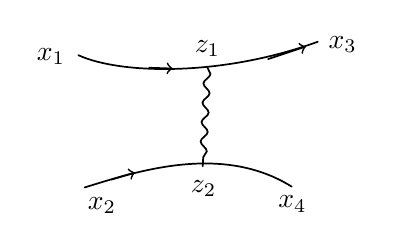
\begin{tikzpicture}[x=1cm,y=1cm,line width=.62pt,line cap=round]
\draw (0,1.90) .. controls (.52,1.66) and (1.8,1.62) .. (3.04,2.07);
\draw[->] (.90,1.74)--(1.20,1.73);
\draw[->] (2.41,1.85)--(2.89,2.01);
\draw (.08,.22) .. controls (.76,.43) and (1.83,.78) .. (2.71,.23);
\draw[->] (.42,.32)--(.72,.41);
\draw[decorate,decoration={snake,amplitude=1.2pt,segment length=7pt}] (1.64,1.74)--(1.58,.49);
\node[left] at (-.04,1.88) {$x_1$}; \node[right] at (3.05,2.03) {$x_3$};
\node[below] at (.30,.22) {$x_2$}; \node[below] at (2.72,.24) {$x_4$};
\node[above] at (1.64,1.75) {$z_1$}; \node[below] at (1.59,.44) {$z_2$};
\end{tikzpicture}}\endgroup\par}
\end{GelfandAdjacentEvidence}
\begin{GelfandAdjacentEvidence}{GELFAND-P000608}{5}

Излуч. и поглощ. фотона сопров. множителем \(e\).
\[
\begin{aligned}
\int &K(x_3-z_1)K(z_1-x_1)K(x_4-z_2)K(z_2-x_2)\\
 &\qquad D(z_2-z_1)\,d^4z_1\,d^4z_2
\end{aligned}
\]
\(D\) — фунд. реш. ур-й Максвелла.

Другие картинки:
\SourceFigure{GELFAND-P000608}{graph-series}{%
\par\smallskip
\begingroup\color{black}\GelfandFitDiagram{\begin{tikzpicture}[x=.62cm,y=.62cm,line width=.55pt,line cap=round,
 photon/.style={decorate,decoration={snake,amplitude=.75pt,segment length=4pt}}]
\draw (0,1.22) .. controls (.28,.84) and (.73,.83) .. (1.39,1.24);
\draw[->] (.62,.95)--(.83,.98);
\draw (.02,.08) .. controls (.38,.22) and (.76,.50) .. (1.23,.08);
\draw[->] (.48,.25)--(.69,.27);
\node at (1.72,.64) {$+$};
\begin{scope}[xshift=1.31cm]
\draw (0,1.16) .. controls (.38,.95) and (1.0,.93) .. (1.43,1.28);
\draw[->] (.48,1.03)--(.64,1.04); \draw[->] (1.13,1.13)--(1.34,1.23);
\draw (0,.02) .. controls (.37,.27) and (1.03,.20) .. (1.38,.13);
\draw[->] (.40,.16)--(.57,.18);
\draw[photon] (.76,1.04)--(.75,.19);
\end{scope}
\node at (3.86,.64) {$+$};
\begin{scope}[xshift=2.61cm]
\draw (0,1.17) .. controls (.24,.89) and (.83,1.00) .. (1.33,1.30);
\draw (.08,.05) .. controls (.45,.20) and (.87,.33) .. (1.31,.12);
\draw (.43,1.04) .. controls (.83,.98) and (.54,.43) .. (.83,.40)
 .. controls (1.01,.40) and (.97,.34) .. (1.02,.23);
\draw (.99,1.11) .. controls (.64,.87) and (.75,.65) .. (.56,.44)
 .. controls (.40,.27) and (.25,.13) .. (.35,.04);
\end{scope}
\node at (5.73,.64) {$+$};
\begin{scope}[xshift=3.82cm]
\draw (0,1.17) .. controls (.26,.88) and (.92,.86) .. (1.36,1.12);
\draw (0,.02) .. controls (.38,.29) and (.92,.30) .. (1.28,.07);
\draw[photon] (.61,.96)--(.62,.68);
\draw (.62,.68) .. controls (.25,.48) and (.70,.40) .. (.84,.61)
 .. controls (.91,.77) and (.52,.72) .. (.72,.53);
\draw[photon] (.66,.47)--(.69,.25);
\node[font=\tiny,align=center,below] at (.69,0) {рожд.\\пары.};
\end{scope}
\node at (7.81,.64) {$+$};
\begin{scope}[xshift=5.08cm]
\draw (0,1.09) .. controls (.48,1.13) and (1.12,1.03) .. (1.35,1.17);
\draw (-.03,.05)--(1.39,.10);
\draw[photon] (.45,1.01)--(.46,.08);
\draw[photon] (.87,1.00)--(.86,.21);
\end{scope}
\node at (9.91,.64) {$+$};
\begin{scope}[xshift=6.38cm]
\draw (0,1.07) .. controls (.28,.97) and (.96,1.01) .. (1.27,1.09);
\draw (.04,1.09)--(.12,1.25)--(.22,1.27)--(.32,1.39)--(.45,1.35)
 --(.57,1.43)--(.61,1.34)--(.79,1.35)--(.82,1.16)--(.85,1.03);
\draw[photon] (.49,1.00)--(.49,.01);
\draw (-.08,.02) .. controls (.36,-.01) and (.95,-.05) .. (1.13,.05);
\end{scope}
\end{tikzpicture}}\endgroup\par
Точки пересечения штрихов в третьей схеме и направление петли в четвёртой неясны.}
\end{GelfandAdjacentEvidence}
\begin{GelfandAdjacentEvidence}{GELFAND-P000608}{6}

\[
(\gamma_\mu p_\mu-m)K(p)=1
\]
\[
K(p)=\frac{\gamma_\mu p_\mu+m}{\underline p^{\,2}-m^2}
\]
\[
K(x,x')=\int K(p)e^{ip(x-x')}\,d^4p
\]
Полюс обх. если взять \(K(p)=\dfrac{\gamma_\mu p_\mu+m}{\underline p^{\,2}-m^2+i0}\)
\Unclear{GELFAND-P000608}{pole-denominator}{Последний знак разомкнут, прочитан как нуль.}
\end{GelfandAdjacentEvidence}
\begin{GelfandAdjacentEvidence}{GELFAND-P000608}{7}

\[
\underline{\underline p^{\,2}=E^2-\vec p^{\,2}}.
\]
\SourceFigure{GELFAND-P000608}{pole-axes}{%
\par\smallskip
\begingroup\color{black}\GelfandFitDiagram{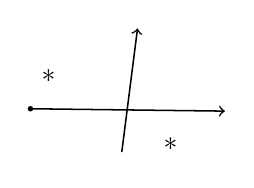
\begin{tikzpicture}[x=1cm,y=1cm,line width=.55pt]
\draw[->] (-1.25,.03)--(1.22,0);
\fill (-1.25,.03) circle (1pt);
\draw[->] (-.09,-.52)--(.11,1.05);
\node at (-1.02,.44) {$\ast$}; \node at (.53,-.42) {$\ast$};
\end{tikzpicture}}\endgroup\par}
\end{GelfandAdjacentEvidence}
\begin{GelfandAdjacentEvidence}{GELFAND-P000608}{8}

Есть уровни с отр. энергией, еств. распр. назад по времени (предсказ. сущ. античастиц).
\Unclear{GELFAND-P000608}{negative-energy-reading}{Сокращение после «энергией» предположительно читается «еств.».}
\end{GelfandAdjacentEvidence}
\begin{GelfandAdjacentEvidence}{GELFAND-P000608}{9}


Сущ. единств. выбор обхода, прив. к согласов. теории: — ни иметь античастиц
\Unclear{GELFAND-P000608}{terminal-words}{Две последние строки сближены. Чтение «ни иметь античастиц» предположительно.}
\end{GelfandAdjacentEvidence}



\Needspace{7\baselineskip}
\begin{GelfandAdjacentEvidence}{GELFAND-P000609}{1}
\SourcePage{GELFAND-P000609}{unlabelled}
\underline{Нормировка заряда}.

\(e\) — явл. ли наблюд. зарядом электрона?

\dashuline{Рассеяние}: электроны обм. фотонами, сила \(\sim e^2\)
\SourceFigure{GELFAND-P000609}{leading-exchange}{%
\par\smallskip
\begingroup\color{black}\GelfandFitDiagram{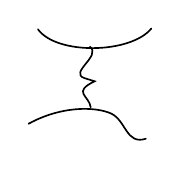
\begin{tikzpicture}[x=1cm,y=1cm,line width=.60pt,line cap=round]
\draw (0,1.35) .. controls (.24,1.02) and (1.18,1.04) .. (1.44,1.36);
\draw (-.12,.15) .. controls (.30,.38) and (.73,.37) .. (.93,.28)
 .. controls (1.12,.19) and (1.12,-.12) .. (1.37,-.04);
\draw (.66,1.13) .. controls (.81,1.01) and (.39,.80) .. (.59,.73)
 --(.72,.69) .. controls (.43,.55) and (.65,.51) .. (.67,.36);
\end{tikzpicture}}\endgroup\par}
\end{GelfandAdjacentEvidence}
\begin{GelfandAdjacentEvidence}{GELFAND-P000609}{2}


Поправка: \(\sim e^4\).
\SourceFigure{GELFAND-P000609}{correction-loop}{%
\par\smallskip
\begingroup\color{black}\GelfandFitDiagram{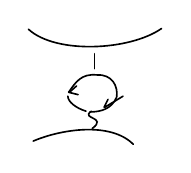
\begin{tikzpicture}[x=1cm,y=1cm,line width=.59pt,line cap=round]
\draw (-.04,1.58) .. controls (.31,1.26) and (1.25,1.31) .. (1.65,1.59);
\draw (.80,1.27)--(.80,1.08);
\draw (.47,.78) .. controls (.56,.91) and (.63,1.02) .. (.83,1.00)
 .. controls (1.02,1.01) and (1.10,.86) .. (1.08,.72)
 .. controls (1.02,.57) and (.88,.53) .. (.74,.53);
\draw (.69,.54) .. controls (.56,.58) and (.46,.66) .. (.46,.73);
\draw (.47,.78)--(.59,.75) (.48,.78)--(.57,.86);
\draw (.92,.59)--(.97,.69) (.93,.59)--(1.16,.73);
\draw (.76,.54) .. controls (.61,.44) and (.97,.47) .. (.77,.32);
\draw (.02,.16) .. controls (.37,.31) and (1.00,.41) .. (1.29,.12);
\end{tikzpicture}}\endgroup\par
Точные направления двух стрелкоподобных штрихов на петле неясны. Видимые зазоры сохранены.}
\end{GelfandAdjacentEvidence}


Наблюд. заряд \(e_{\text{физ}}^2<e^2\).

В теор. сильного взаимод. наоборот \(g_{\text{физ}}^2>g^2\).
\[
\rule{1.8em}{.4pt}\;\boldsymbol{\cdot}\;\rule{1.8em}{.4pt}
\]


\Needspace{7\baselineskip}
\begin{GelfandAdjacentEvidence}{GELFAND-P000610}{1}
\SourcePage{GELFAND-P000610}{unlabelled}
\underline{\underline{22.9.75.}}\qquad\underline{Сем. Гельфанда.}

\SourceFigure{GELFAND-P000610}{scan-comment-mark}{%
\par\smallskip
\begingroup\color{black}\GelfandFitDiagram{
\begin{tikzpicture}[x=1cm,y=1cm,line width=.55pt]
\draw[fill=yellow,rounded corners=2pt] (0,.17)--(0,.74)--(.84,.74)--(.84,.17)--(.42,.17)--(.22,0)--(.26,.17)--cycle;
\draw (.14,.59)--(.70,.59) (.14,.46)--(.70,.46) (.14,.33)--(.56,.33);
\end{tikzpicture}}\endgroup\par
Жёлтый значок комментария в правом верхнем поле цифрового кадра.}
\end{GelfandAdjacentEvidence}
\begin{GelfandAdjacentEvidence}{GELFAND-P000610}{2}


\underline{Гельфанд о рез. Атьи.}

\(\mathfrak A\) — все опер. в гильб. пр-ве, \(\mathcal K\) — комп. опер.
\[
\mathfrak A/\mathcal K=\mathfrak B.
\]
Когда \(B_1,B_2\in\mathfrak B\) унитарно эквивалентны?

Это [зачёркнуто] \uwave{Браун, Дуглас, Филлмор} (Lect. Notes, \(N=\ldots\))
\Unclear{GELFAND-P000610}{cancel-before-brown}{Перед фамилиями зачёркнута запись, возможно «Все».}
\end{GelfandAdjacentEvidence}
\begin{GelfandAdjacentEvidence}{GELFAND-P000610}{3}


а) спектры совп. (сущ.)

б) индексы совп. в [зачёркнуто] \(\forall\) связн. комп. дополнения
\Incomplete{GELFAND-P000610}{cancel-indices}{Перед квантором зачёркнута запись.}
\end{GelfandAdjacentEvidence}
\begin{GelfandAdjacentEvidence}{GELFAND-P000610}{4}


\underline{Теор. 2.} [зачёркнуто] Пусть \(X\) — компакт,
\[
\underset{\substack{\uparrow\\\text{мн-во вложений }C(X)\text{ в }\mathfrak B.}}{\operatorname{Ext}(X)}\cong K_1(X)
\]
\Incomplete{GELFAND-P000610}{cancel-theorem}{Перед «Пусть» зачёркнута запись.}
\end{GelfandAdjacentEvidence}
\begin{GelfandAdjacentEvidence}{GELFAND-P000610}{5}


\[\rule{1.8em}{.4pt}\;\boldsymbol{\cdot}\;\rule{1.8em}{.4pt}\]
\dashuline{Мозер} — \uwave{Кортевег-де-Фрис}
\[\rule{1.8em}{.4pt}\;\boldsymbol{\cdot}\;\rule{1.8em}{.4pt}\]
\dashuline{Костант}
\[
\psi(x)=\prod_{n=1}^{\infty}(1-x^n);\qquad
\psi(x)^{-1}=\sum_{n=0}^{\infty}p(n)x^n
\]
(\(p(n)\) — число разб. числа \(n\)).

Это
\[
\psi(x)=\sum(-1)^n x^{\frac{n^2-3n}{2}}
\]
\Unclear{GELFAND-P000610}{euler-exponent}{В показателе записано \((n^2-3n)/2\).}
\end{GelfandAdjacentEvidence}
\begin{GelfandAdjacentEvidence}{GELFAND-P000610}{6}


\noindent\makebox[0pt][r]{\(\bullet\)\hspace{.7em}}«Наиболее замечат. ф-ла во всей математике» (Якоби).
\Unclear{GELFAND-P000610}{function-abbreviation}{После «замечат.» густо переписано сокращение, предположительно «ф-ла».}
\end{GelfandAdjacentEvidence}
\begin{GelfandAdjacentEvidence}{GELFAND-P000610}{7}

\[
(\psi(x))^3=\sum_{n=0}^{\infty}(-1)^n(2n+1)x^{\frac{n(n+1)}2}
\]
\[
\eta(x)=x^{1/24}\cdot\psi(x).
\]
\[
\eta^{24}(x)=\sum\tau(n)x^n,\qquad\tau(n)\text{ — ф-я Рамануджана}
\]
\(\psi^{10}(x)\) тоже есть

\underline{Манин}: если 6 разных ф-й, получ. из разных соображений
\[
\eta(x)^{\square}=\sum\ldots
\]
Макдональд нашёл показ. степени, при к-рых есть смысл:
Это \(\dim\) компактных групп Ли.
\[
\psi(x)^{\dim K}=\sum_\lambda\text{[зачёркнуто]}\ \chi_\lambda(a)\,\dim V_\lambda\cdot x^{\text{(зав. от }\lambda\text{)}}
\]
\Incomplete{GELFAND-P000610}{cancel-character}{После знака суммы перед \(\chi_\lambda(a)\) зачёркнута запись.}
\end{GelfandAdjacentEvidence}
\begin{GelfandAdjacentEvidence}{GELFAND-P000610}{8}

\(a\in K\), \(\chi_\lambda(a)=\pm1\) или \(0\)

Костант: \(\operatorname{Sp}(-\Delta+a)^{-s}\) и т.д.

\dashuline{Внутр. ч-ие Г.}: \uwave{\(\psi(x)^z\)} — ?\qquad \((z\in\mathbb C)\)
\Unclear{GELFAND-P000610}{inner-abbreviation}{Среднее сокращение предположительно читается «ч-ие».}
\end{GelfandAdjacentEvidence}
\begin{GelfandAdjacentEvidence}{GELFAND-P000610}{9}

\[\rule{1.8em}{.4pt}\;\boldsymbol{\cdot}\;\rule{1.8em}{.4pt}\]
\underline{\underline{Поляков}}. (продолжение).

\underline{Литература}:
\[
\text{\underline{кв. мех.}}\quad\left\{\begin{array}{@{}l@{}}
\text{1) \uwave{Ландау и Лифшиц} (квант. механика).}\ (\approx5\text{–}7\ \text{глав})\\
\text{2) \uwave{Дирак}}\\
\text{3) \uwave{Фейнман} (для школьников)}\\
\text{4) \uwave{Фейнман}. Интегралы по траекториям}
\end{array}\right.
\]
\Unclear{GELFAND-P000610}{bibliography-count}{После «5–7» предположительно написано «глав».}
\end{GelfandAdjacentEvidence}


\underline{Кв. теор. поля}: 1-я часть т. \underline{IV}\quad\dashuline{Берестецкий, Лифшиц, Питаевский}


\Needspace{7\baselineskip}
\begin{GelfandAdjacentEvidence}{GELFAND-P000611}{1}
\SourcePage{GELFAND-P000611}{unlabelled}
\(e(x)\) — поле (биспиноры)
\[
\mathcal L_{\mathrm{free}}=\bar e\,i\gamma_\mu\partial_\mu e
-m\bar e e+\frac1{4e^2}F_{\mu\nu}^2
\]
\[
\mathcal L_{\mathrm{int}}=\ldots\bar e\gamma_\mu e A_\mu\ldots
\qquad\text{сод. 3-… член.}
\]
\Unclear{GELFAND-P000611}{interaction-abbreviation}{Сокращение после «3-» читается неуверенно.}
\end{GelfandAdjacentEvidence}
\begin{GelfandAdjacentEvidence}{GELFAND-P000611}{2}

\[\rule{1.8em}{.4pt}\;\boldsymbol{\cdot}\;\rule{1.8em}{.4pt}\]
\dashuline{Локализация б-их вн. симметрий — слабое взаимод.}
\Unclear{GELFAND-P000611}{heading-abbreviations}{Предположительно «б-их вн.».}
\end{GelfandAdjacentEvidence}
\begin{GelfandAdjacentEvidence}{GELFAND-P000611}{3}

\[
\begin{aligned}
\mathcal L={}&\bar e_L i\gamma_\mu\partial_\mu e_L
+\bar e_R i\gamma_\mu\partial_\mu e_R
+\bar\nu_L i\gamma_\mu\partial_\mu\nu_L+\\
&+\begin{pmatrix}e\to\mu\\ \nu_L\to\nu'_L\end{pmatrix}
+m(\bar e_L e_R+\bar e_R e_L).
\end{aligned}
\]
(все лептоны)\quad\(\downarrow\)

\(\nu'_L\) — \(\mu\)-мезонное нейтрино
\[
\mathcal L=\bar e_L i\gamma_\mu\partial_\mu e_L
+\bar\nu_L i\gamma_\mu\partial_\mu\nu_L
+\bar e_R i\gamma_\mu\partial_\mu e_R
\]
\[
\left\{
\begin{aligned}
\begin{pmatrix}e'_L\\\nu'_L\end{pmatrix}
&=U\begin{pmatrix}e_L\\\nu_L\end{pmatrix}
\qquad SU_L(2)\\
e'_R&=e_R
\end{aligned}
\right.
\]
\hfill\(\bullet\)

Возн. новая гр. симметрии \(SU(2)\) и ещё \(U(1)\)
\[
F=SU_L(2)\times U_R(1)\times U_L(1)
\quad\text{— общая лептонная группа.}
\]
\[
\begin{pmatrix}e_L\\\nu_L\end{pmatrix}
\overset{U_L(1)}{\longrightarrow}
e^{i\gamma}\begin{pmatrix}e_L\\\nu_L\end{pmatrix}
\]
\Unclear{GELFAND-P000611}{phase-letter}{Буква в фазе предположительно \(\gamma\), возможно \(\delta\).}
\end{GelfandAdjacentEvidence}
\begin{GelfandAdjacentEvidence}{GELFAND-P000611}{4}


\dashuline{Локализация}

\Incomplete{GELFAND-P000611}{cancel-left}{Зачёркнутая запись в рамке в левом поле не читается.}
\end{GelfandAdjacentEvidence}
\begin{GelfandAdjacentEvidence}{GELFAND-P000611}{5}


[Зачёркнуто: \sout{\(A_\mu\) … эл. магн. поле}.]
\Unclear{GELFAND-P000611}{cancel-a}{Между \(A_\mu\) и «эл. магн. поле» виден знак, скрытый штрихами.}
\end{GelfandAdjacentEvidence}
\begin{GelfandAdjacentEvidence}{GELFAND-P000611}{6}


Ковар. произв. для \(SU(2)\).
\qquad \(\bar\tau\) — матр. Паули (3 шт.)
\[
\begin{pmatrix}e'_L\\\nu'_L\end{pmatrix}
=e^{i\frac{\vec\tau\vec\alpha(x)}2}
\begin{pmatrix}e_L\\\nu_L\end{pmatrix},
\qquad E'=e^{i\frac{\bar\tau\bar\alpha(x)}2}E
\]
\Unclear{GELFAND-P000611}{doublet-overwrite}{Нижняя буква слева и нижний индекс справа переписаны.}
\end{GelfandAdjacentEvidence}
\begin{GelfandAdjacentEvidence}{GELFAND-P000611}{7}

Инфинитезим.:
\[
E'=\left(1-\frac i2(\bar\tau\bar\alpha)\right)E
\]
\Unclear{GELFAND-P000611}{finite-infinitesimal-sign}{В показателе конечного преобразования знак плюса подразумевается, в инфинитезимальной записи виден минус.}
\end{GelfandAdjacentEvidence}

\[
\partial_\mu E'=
\left(1-\frac i2(\bar\tau\bar\alpha)\right)\partial_\mu E
-\frac i2(\bar\tau\partial_\mu\bar\alpha)E
\]
\[
\fbox{$\displaystyle\nabla_\mu E
=\partial_\mu E+\frac i2(\vec\tau\vec A_\mu)E$}
\]
\[
E'=e^{i\frac{\bar\tau\bar\alpha(x)}2}E
\]
\[
\nabla_\mu E'=e^{i\frac{\bar\tau\bar\alpha}2}\nabla_\mu E
\]
Здесь возник. 3 безмасс. частицы


\Needspace{7\baselineskip}
\begin{GelfandAdjacentEvidence}{GELFAND-P000612}{1}
\SourcePage{GELFAND-P000612}{unlabelled}
можно сразу писать
\[
\nabla_\mu E^\delta=\partial_\mu E^\delta+A_\mu^{\delta\beta}E^\beta
\]
\Unclear{GELFAND-P000612}{upper-component-index}{Верхний индекс предположительно \(\delta\), возможно \(\gamma\).}
\end{GelfandAdjacentEvidence}
\begin{GelfandAdjacentEvidence}{GELFAND-P000612}{2}

и смотрим, как преобр. \(A\), чтобы \(\nabla_\mu E^\delta\) преобр. как \(E^\delta\).

\[
\begin{aligned}
\mathcal L_{\mathrm{вз}}={}&(\bar e_i\gamma_\mu\nu_e)A_\mu^{(-)}
+(\bar\nu_e\gamma_\mu e_i)A_\mu^{(+)}\\
&+(\bar e_L\gamma_\mu e_L-\bar\nu_L\gamma_\mu\nu_L)A_\mu^3
\end{aligned}
\]
\Unclear{GELFAND-P000612}{weak-electron-index}{В первых двух слагаемых у электрона виден индекс \(i\) с точкой.}
\end{GelfandAdjacentEvidence}
\begin{GelfandAdjacentEvidence}{GELFAND-P000612}{3}

где
\[
A_\mu^\pm=A_\mu^1\pm iA_\mu^2
\]
Пример слабого взаимод.: \(\mu^-\to e^-,\bar\nu_e,\nu_\mu.\)
\[
\mathcal L=\bar E\left(i\gamma_\mu\frac{\partial E}{\partial x_\mu}\right)
+\underset{\mathcal L_{\mathrm{вз}}}{\tikz[baseline=(term.base)]{
\node[inner sep=0pt] (term) {$\bar E\gamma_\mu\vec\tau E\vec A_\mu$};
\draw ([yshift=-.2ex]term.south west) -- ([yshift=-.75ex]term.south west)
-- ([yshift=-.75ex]term.south east) -- ([yshift=-.2ex]term.south east);
}}
+\bar e_R i\gamma_\mu\partial_\mu e_R
\]
\Unclear{GELFAND-P000612}{lagrangian-mark}{Слева от \(\mathcal L\) виден отдельный короткий штрих с точками. Его значение неясно.}
\end{GelfandAdjacentEvidence}
\begin{GelfandAdjacentEvidence}{GELFAND-P000612}{4}

\Incomplete{GELFAND-P000612}{cancel-underbrace}{Под скобкой слева зачёркнута запись.}
\end{GelfandAdjacentEvidence}
\begin{GelfandAdjacentEvidence}{GELFAND-P000612}{5}

\Incomplete{GELFAND-P000612}{cancel-right}{Отдельная зачёркнутая запись в правом поле не читается.}
\end{GelfandAdjacentEvidence}
\begin{GelfandAdjacentEvidence}{GELFAND-P000612}{6}


\[\rule{1.8em}{.4pt}\;\boldsymbol{\cdot}\;\rule{1.8em}{.4pt}\]
Ещё локализуем пр. поле
\Unclear{GELFAND-P000612}{right-field-abbreviation}{Сокращение «пр.» предположительно означает «правое».}
\end{GelfandAdjacentEvidence}
\begin{GelfandAdjacentEvidence}{GELFAND-P000612}{7}

\[
\begin{aligned}
&\bar E\left(i\gamma_\mu\frac{\partial E}{\partial x_\mu}\right)
+\bar E\gamma_\mu\vec\tau E\vec A_\mu
+\bar e_R i\gamma_\mu\partial_\mu e_R\\
&\qquad+\bar e_R\gamma_\mu e_R B_\mu
\end{aligned}
\]
\[
A_\mu=A_\mu^3\cos\theta+B_\mu\sin\theta
\]
\[\boldsymbol{\cdot}\;\cdot\;\cdot\;\cdot\;\cdot\;\cdot\;{\scriptscriptstyle-}\;
\cdot\;\cdot\;\cdot\;\cdot\;\cdot\]
След. раз — \(\approx\) \underline{через 3 недели.}

\textbf{12 кварков:} \uwave{4 сорта и 3 цвета.}

\SourceFigure{GELFAND-P000612}{scan-comment-mark}{%
\par\smallskip
\begingroup\color{black}\GelfandFitDiagram{
\begin{tikzpicture}[x=1cm,y=1cm,line width=.55pt]
\draw[fill=yellow,rounded corners=2pt] (0,.17)--(0,.74)--(.84,.74)--(.84,.17)--(.42,.17)--(.22,0)--(.26,.17)--cycle;
\draw (.14,.59)--(.70,.59) (.14,.46)--(.70,.46) (.14,.33)--(.56,.33);
\end{tikzpicture}}\endgroup\par
Жёлтый значок комментария справа от строки о кварках в цифровом кадре.}
\end{GelfandAdjacentEvidence}

\[\rule{1.8em}{.4pt}\;\boldsymbol{\cdot}\;\rule{1.8em}{.4pt}\]


\Needspace{7\baselineskip}
\begin{GelfandAdjacentEvidence}{GELFAND-P000613}{1}
\SourcePage{GELFAND-P000613}{unlabelled}
\uuline{29.9.75.}\qquad\uuline{Сем. Гельфанда.}

\uuline{Ю. И. Манин.}
\[
x\prod_{n=1}^\infty(1-x^n)^{24}=\sum_{n=1}^\infty\tau(n)x^n;
\qquad \tau\text{ — ф-я Рамануджана}.
\]
\underline{И. М. Гельфанд}. (и Дикий)

\(\infty\)\uwave{-мерная алгебра Ли, более замеч., чем все картановские}.

Элементы — полиномы \(P(u,u',\ldots,u^{(n)})\) от любого числа переменных.

\(P\overset{\prime\prime}{[}u]\), где \(u=\{u,u',\ldots,u^{(n)},\,\cdot\,\}\)
\Unclear{GELFAND-P000613}{formal-variable-mark}{Два штриха стоят над левой частью квадратной скобки.}
\end{GelfandAdjacentEvidence}
\begin{GelfandAdjacentEvidence}{GELFAND-P000613}{2}


Есть понятие
\[
\frac{d}{dx}P(u,u',\ldots,u^{(n)})
=\sum_{i=0}^\infty\frac{\partial P}{\partial u^{(i)}}\cdot u^{(i+1)}
\]
Есть умножение (алгебр.)

Неожиданно: есть понятие \underline{коммутатора}:
\[
[P,Q]=\sum_{k=0}^\infty
\left[\left(\frac{d}{dx}\right)^kP\cdot\frac{\partial Q}{\partial u^{(k)}}
-\left(\frac{d}{dx}\right)^kQ\cdot\frac{dP}{du^{(k)}}\right]
\]
\Unclear{GELFAND-P000613}{commutator-separator}{Знак после \(Q\) читается как точка умножения. В последней дроби написано \(d\).}
\end{GelfandAdjacentEvidence}
\begin{GelfandAdjacentEvidence}{GELFAND-P000613}{3}

\Unclear{GELFAND-P000613}{cancelled-speaker}{Короткая запись перед фамилией зачёркнута.}
\end{GelfandAdjacentEvidence}
\begin{GelfandAdjacentEvidence}{GELFAND-P000613}{4}

\Incomplete{GELFAND-P000613}{cancelled-speaker-loss}{Зачёркнутая запись целиком не читается.}
\end{GelfandAdjacentEvidence}
\begin{GelfandAdjacentEvidence}{GELFAND-P000613}{5}


\uuline{Повзнер}. Эта ал. связ. с ур-ем \(\dfrac{\partial u}{\partial t}=\dfrac{\partial u}{\partial x}\).
Можно связ. с \(\forall\) ур-ем
\[
\frac{\partial u}{\partial t}=a(u,u_x,\ldots).
\]
Рассм. ф-и \(F(u,u_x,\ldots)\) и оператор
\[
a[F(u,u_x,\ldots)]=aF_u+\left(\frac{d}{dx}a\right)F_{u_x}
+\frac{d^2a}{dx^2}F_{u_{xx}}+\ldots
\]
Оператор опр. по ф-и \(a\) и стр. алгебра из этих опер.
\[
[a,b]=a[b]-b[a]\text{ — та же алгебра}.
\]
\[\rule{1.8em}{.4pt}\;\boldsymbol{\cdot}\;\rule{1.8em}{.4pt}\]
Здесь указано естественное предст. этой алгебры.
\Unclear{GELFAND-P000613}{representation-marginal-mark}{Слева от «Здесь» зачернён знак.}
\end{GelfandAdjacentEvidence}
\begin{GelfandAdjacentEvidence}{GELFAND-P000613}{6}

\[\rule{1.8em}{.4pt}\;\boldsymbol{\cdot}\;\rule{1.8em}{.4pt}\]
\uuline{Манин}. 6 выражений для ф-и Рамануджана \(\tau(n)\) (не получ. конечным алгоритмом).

\textcircled{\scriptsize +}\quad\textcircled{\scriptsize 1}\quad\underline{Определение} \(\Rightarrow\)
\[
\tau(n)=\sum(-1)^k
\]
\[
\begin{gathered}
n-1=n_1+\ldots+n_k,\qquad n_i\ge1\\
n_1\le n_2\le\ldots\le n_k
\end{gathered}
\]
подряд \(\le24\) знаков рав-ва.

\textcircled{\scriptsize +}\quad\textcircled{\scriptsize 2}\quad\uwave{Макдональд} (\uwave{Дайсон})
\[
\tau(n)=\frac1{1!2!3!4!}\sum\prod_{i<j}(u_i-u_j)
\]
\Unclear{GELFAND-P000613}{vandermonde-relation}{Под знаком произведения предположительно \(i<j\).}
\end{GelfandAdjacentEvidence}
\begin{GelfandAdjacentEvidence}{GELFAND-P000613}{7}

\[
10n=\sum_{i=1}^5u_i^2,\qquad\sum u_i=0,\qquad u_i\equiv i\bmod5
\]

\(\left(\begin{smallmatrix}+\\+\end{smallmatrix}\right)\)
\quad\textcircled{\scriptsize 3}\quad\uwave{Рамануджан}
\[
\tau(n)=\frac{65}{756}\sigma_{11}(n)+\frac{691}{756}\sigma_5(n)
-\frac{691}{3}\sum_{m=1}^{n-1}\sigma_5(m)\sigma_5(n-m)
\]
\Unclear{GELFAND-P000613}{ramanujan-denominator}{Последняя цифра в первом знаменателе переписана и читается как 6.}
\end{GelfandAdjacentEvidence}
\begin{GelfandAdjacentEvidence}{GELFAND-P000613}{8}

\Unclear{GELFAND-P000613}{ramanujan-convolution}{В последнем множителе читается \(n-m\).}
\end{GelfandAdjacentEvidence}

\(\sigma_k(n)\) — \(\sum\) \(k\)-х степ. делителей числа \(n\).

\underline{Следствие:} \(\tau(n)\equiv\sigma_{11}(n)\bmod691\).
(угадал Рамануджан).


\Needspace{7\baselineskip}
\begin{GelfandAdjacentEvidence}{GELFAND-P000614}{1}
\SourcePage{GELFAND-P000614}{unlabelled}
\textcircled{\scriptsize 4}\quad Цел. кв. форм с \(\det=1\) от 24 перем.
\hfill Всего 2.

\(\left(\begin{smallmatrix}+\\+\end{smallmatrix}\right)\)
\qquad Пусть \(Q_{24}\) — одна из них.
\Unclear{GELFAND-P000614}{form-count}{В строке указано «Всего 2».}
\end{GelfandAdjacentEvidence}
\begin{GelfandAdjacentEvidence}{GELFAND-P000614}{2}

\[
\tau(n)=\alpha\left(\sum_{Q_{24}=n}1\right)-\beta\sigma_{11}(n)
\]
(\(\alpha,\beta\) вычисл. из \(n=1\) и \(2\)).

\textcircled{\scriptsize 5}\quad (Манин)
\hspace{1em}\(\left(\begin{smallmatrix}+\\+\end{smallmatrix}\right)\)
\[
\tau(n)=\sigma_{11}(n)-\sum_{n=\Delta\Delta'+\delta\delta'}'
\left[(\Delta^8\delta^2-\Delta^2\delta^8)
+\frac{691}{6}(\Delta^6\delta^4-\Delta^4\delta^6)\right],
\]
\Unclear{GELFAND-P000614}{manin-primed-sum}{У знака суммы виден штрих.}
\end{GelfandAdjacentEvidence}
\begin{GelfandAdjacentEvidence}{GELFAND-P000614}{3}

\[
\begin{gathered}
\Delta>\delta>0,\quad\text{и }\bigl[\,\Delta'>\delta'>0\quad(\text{целые})\\
\text{или }\Delta\mid n,\quad \Delta'=\frac n\Delta,\quad
\delta'=0,\quad0<\frac\delta\Delta\le\frac12\,\bigr].
\end{gathered}
\]

\textcircled{\scriptsize 6}\quad
\(\left(\begin{smallmatrix}+\\+\\+\end{smallmatrix}\right)\)
\[
\sum p(n)x^n=\prod_{n=1}^\infty(1-x^n)^{-1}
\]
(\(p(n)\) — число разбиений \(n\) на произв. число слаг.).
\[
\Rightarrow\quad \sum\tau(n)x^n=x\left(\sum_{n=1}^{\infty}p(n)x^n\right)^{-24}
\]
\Unclear{GELFAND-P000614}{partition-inner-start}{Нижняя граница внутренней суммы написана \(n=1\).}
\end{GelfandAdjacentEvidence}
\begin{GelfandAdjacentEvidence}{GELFAND-P000614}{4}

Через \(p(n)\) рекурс. нах. \(\tau(n)\).

Ф-ла Харди–Рамануджана–Радемахера
\[
p(n)=\frac1{\sqrt3}\sum_{k=1}^{\infty}\frac1{\sqrt k}
\sum_{\substack{h\bmod k\\(h,k)=1}}
\omega_{h,k}e^{-2\pi i n\frac1k}\cdot
\frac d{dn}\frac{\operatorname{sh}\frac\pi{6k}\sqrt{24n-1}}
{\frac\pi{6k}\sqrt{24n-1}}
\]
\Unclear{GELFAND-P000614}{hrr-omega-exponential}{В показателе написано \(1/k\).}
\end{GelfandAdjacentEvidence}
\begin{GelfandAdjacentEvidence}{GELFAND-P000614}{5}

\(\omega_{h,k}^{24}=1\) тоже есть для \(\omega_{h,k}\) явные ф-лы.

Харди–Раманудж. написали [зачёркнуто] \(\operatorname{sh}\to e^{\ldots}\).
\Incomplete{GELFAND-P000614}{hrr-cancelled-prefix}{Перед «sh» зачёркнута короткая запись.}
\end{GelfandAdjacentEvidence}
\begin{GelfandAdjacentEvidence}{GELFAND-P000614}{6}

[Под \(\operatorname{sh}\to e^{\ldots}\): расходится.]
но если оборвать на члене \(\sqrt n\), то приближает хорошо.
На \(\sqrt n\) членов надо остановиться.
Каждая из этих ф-л — часть беск. серии формул.

\textcircled{\scriptsize 7}\quad
\(\left(\begin{smallmatrix}+\\+\end{smallmatrix}\right)\)
\qquad \uuline{\(\tau(mn)=\tau(m)\tau(n)\)}, \((m,n)=1\)

(не видно из ф-л).
\[
\tau(p)=\theta_p+\bar\theta_p,\qquad\theta_p\bar\theta_p=p^{11}
\quad\Rightarrow
\]
\begin{center}
\uuline{\(\tau(p^a)=\theta_p^a+\bar\theta_p^a.\)}
\end{center}
\Unclear{GELFAND-P000614}{theta-power}{Дважды подчёркнутая формула приведена в написанном виде.}
\end{GelfandAdjacentEvidence}
\begin{GelfandAdjacentEvidence}{GELFAND-P000614}{7}

В каждую из ф-л можно подст. и получ. новые тожд.

\textcircled{\scriptsize 8}\quad
\(\left(\begin{smallmatrix}+\\+\\+\\+\end{smallmatrix}\right)\)
\qquad Отсюда [обведённая вставка: подозрение, что] \(\tau\) — след представления (намного труднее) — Серр, Делинь.
\Unclear{GELFAND-P000614}{suspicion-insertion}{Обведённая вставка читается «подозрение, что».}
\end{GelfandAdjacentEvidence}
\begin{GelfandAdjacentEvidence}{GELFAND-P000614}{8}

Гротендик, Вейль, Куга, Сато, [зачёркнуто] Ранкин.
\Incomplete{GELFAND-P000614}{cancelled-author}{Зачёркнутая запись перед фамилией Ранкин не читается.}
\end{GelfandAdjacentEvidence}
\begin{GelfandAdjacentEvidence}{GELFAND-P000614}{9}

Предст. \(\ell\)-адическое
\[
\operatorname{Gal}_{\{\ell\}}(\bar Q/Q)\longrightarrow Q_\ell^2
\]
(разветвл. только в \(\ell\)).
След бер. от авт. Фробениуса, порожд. \(p\).

Отсюда удалось док., что \uuline{\(\theta_p\) чисто мнимые} (невеществ.)
\Unclear{GELFAND-P000614}{theta-imaginary}{Чтение «чисто мнимые» сохранено.}
\end{GelfandAdjacentEvidence}

\(\longrightarrow\) Самая длинная теор. в соврем. математике (Оценка Делиня: 2000 страниц).


\Needspace{7\baselineskip}
\begin{GelfandAdjacentEvidence}{GELFAND-P000615}{1}
\SourcePage{GELFAND-P000615}{unlabelled}
\underline{Уровни трудности.}
\[
\begin{array}{cl}
+&\text{комбинаторика}\\
++&\text{модулярные формы}\\
+++&\text{комплексный анализ}\\
++++&\text{алг. геом. и т.п., этальные когом. и пр.}\\\hline
\end{array}
\]
\[\rule{1.8em}{.4pt}\;\boldsymbol{\cdot}\;\rule{1.8em}{.4pt}\]

\underline{Как получается.}
\[
\eta(z)=e^{\frac{2\pi inz}{24}}\prod(1-e^{2\pi inz})
\]
\Unclear{GELFAND-P000615}{eta-prefactor}{В показателе множителя написано \(2\pi inz/24\).}
\end{GelfandAdjacentEvidence}
\begin{GelfandAdjacentEvidence}{GELFAND-P000615}{2}

Положим \(x=e^{\frac{2\pi inz}{24}}\).
\Unclear{GELFAND-P000615}{x-definition}{Между \(i\) и \(z\) виден густой знак, предположительно \(n\). Знаменатель переписан.}
\end{GelfandAdjacentEvidence}
\begin{GelfandAdjacentEvidence}{GELFAND-P000615}{3}

Ф-я хорошо ведёт [зачёркнуто] себя при подст.
\(z\to\dfrac{az+b}{cz+d}\),
\(\begin{vmatrix}a&b\\c&d\end{vmatrix}=1\).
\Incomplete{GELFAND-P000615}{verb-cancelled}{После «ведёт» зачёркнуты короткие штрихи.}
\end{GelfandAdjacentEvidence}
\begin{GelfandAdjacentEvidence}{GELFAND-P000615}{4}

\[
\begin{aligned}
\eta(z+1)&=e^{\pi i/12}\eta(z),\\
\eta(-1/z)&=\sqrt{z/i}\,\eta(z).
\end{aligned}
\]
или \(\eta^{24}(\tau)(d\tau)^6\) — инв-на отн. др.-лин. подст..
\Unclear{GELFAND-P000615}{eta-differential}{У \(d\tau\) написана степень \(6\).}
\end{GelfandAdjacentEvidence}
\begin{GelfandAdjacentEvidence}{GELFAND-P000615}{5}


Потеря инф. — \(\sqrt[24]{\ldots}=\omega_{c,d}\) — те же.
\[
\begin{pmatrix}a,&\bar b\\c,&d\end{pmatrix}
\]
\Unclear{GELFAND-P000615}{matrix-mark}{В матрице под «Потеря инф.» над \(b\) видна отдельная черта.}
\end{GelfandAdjacentEvidence}
\begin{GelfandAdjacentEvidence}{GELFAND-P000615}{6}

Ф-и так. вида (модулярные) — кольцо с 2-мя образ., и надо запис. через образующие, [зачёркнуто \sout{или}]
Тожд. в кольце \(\Rightarrow\) рав. в коэфф. Фурье
(\(\Rightarrow\) \textcircled{\scriptsize 3}, \textcircled{\scriptsize 4}).
\Unclear{GELFAND-P000615}{or-cancelled}{Над строкой зачёркнуто слово, предположительно «или».}
\end{GelfandAdjacentEvidence}
\begin{GelfandAdjacentEvidence}{GELFAND-P000615}{7}


\uuline{Чистая алгебра:}
\[
\left\{\varphi(z)\mathrel{\Big|}\sum_{n=0}^\infty a_ne^{2\pi inz}\right\},
\qquad
\exists k:\quad \varphi(z)dz^k\mathrel{\Big|}\begin{pmatrix}a&b\\c&d\end{pmatrix}
=\varphi(z)dz^k.
\]
\(\longleftarrow\) сход. ряд при \(\operatorname{Im}z>0\).

\underline{Т-ма:} кольцо \(\Phi=C[E_4,E_6]\).
\[
\begin{aligned}
a_n|_{E_4}&=\sigma_3(n)\\
a_n|_{E_6}&=\sigma_5(n)
\end{aligned}
\Bigg\Vert\qquad \sigma_3\text{ — суммы кубов делит.}.
\]
\[\rule{1.8em}{.4pt}\;\boldsymbol{\cdot}\;\rule{1.8em}{.4pt}\]

\underline{Х. Р. Р.} (ф-ла 6).
\[
\sum p(n)e^{2\pi inz}=\frac1{\prod(1-e^{2\pi izn})}.
\]
Особ. точки на гр. сходимости (полюсы \(\infty\) пор. в рац. точках).

Контур интегр. Радемахера: у \(\forall\) рац. точки круги опр. радиуса.
\SourceFigure{GELFAND-P000615}{circle-contour}{%
\par\smallskip
\begingroup\color{black}\GelfandFitDiagram{\begin{tikzpicture}[x=1.65cm,y=1.65cm,line width=.55pt]
\draw (-.51,0)--(1.49,.015);
\draw (0,0) .. controls (-.24,0) and (-.49,.28) .. (-.49,.48)
 .. controls (-.51,.82) and (-.32,.94) .. (.03,.97)
 .. controls (.25,1.01) and (.49,.71) .. (.5,.51)
 .. controls (.50,.29) and (.26,0) .. (0,0);
\draw (1,0) .. controls (.78,0) and (.51,.21) .. (.51,.44)
 .. controls (.49,.67) and (.75,.92) .. (1.04,.91)
 .. controls (1.28,.93) and (1.48,.71) .. (1.48,.51)
 .. controls (1.48,.24) and (1.21,0) .. (1,0);
\draw (.5,.13) ellipse [x radius=.115,y radius=.115];
\draw (.30,.012) .. controls (.33,.17) and (.41,.10) .. (.42,.012);
\draw (.59,.014) .. controls (.63,.115) and (.68,.105) .. (.71,.014);
\node[below] at (0,0) {\(0\)};
\node[below] at (.5,0) {\(\tfrac12\)};
\node[below] at (1,0) {\(1\)};
\end{tikzpicture}}\endgroup\par
Точная форма коротких дуг около малого круга неясна.}
\end{GelfandAdjacentEvidence}
\begin{GelfandAdjacentEvidence}{GELFAND-P000615}{8}

\SourceFigure{GELFAND-P000615}{contour-first-approximation}{%
\par\smallskip
\begingroup\color{black}\GelfandFitDiagram{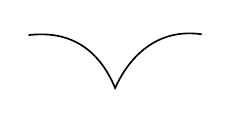
\begin{tikzpicture}[x=1.1cm,y=1.05cm,line width=.6pt]
\draw (0,.64) .. controls (.47,.70) and (.81,.48) .. (1,0)
 .. controls (1.20,.46) and (1.55,.72) .. (2,.65);
\end{tikzpicture}}\endgroup\par
— 1-е прибл.}
\end{GelfandAdjacentEvidence}
\begin{GelfandAdjacentEvidence}{GELFAND-P000615}{9}

\SourceFigure{GELFAND-P000615}{contour-second-approximation}{%
\par\smallskip
\begingroup\color{black}\GelfandFitDiagram{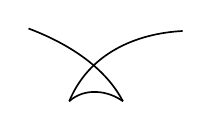
\begin{tikzpicture}[x=1.1cm,y=1.05cm,line width=.6pt]
\draw (0,.88) .. controls (.38,.73) and (.86,.46) .. (1.09,0);
\draw (.47,0) .. controls (.70,.58) and (1.24,.82) .. (1.78,.85);
\draw (.47,0) .. controls (.65,.17) and (.92,.13) .. (1.09,0);
\end{tikzpicture}}\endgroup\par
— 2-е прибл.}
\end{GelfandAdjacentEvidence}
\begin{GelfandAdjacentEvidence}{GELFAND-P000615}{10}

и т.д.
\par\smallskip\noindent\rule{\linewidth}{.35pt}\par

Частн. случай ф-л Макдональда в преобр. Костантом виде:
\[
\varphi(x)=\prod_{n=1}^\infty(1-x^n),\qquad
\varphi(x)=\sum_{\lambda\in D}\chi_\lambda(a)\dim V_\lambda\,x^{c(\lambda)}.
\]
\Incomplete{GELFAND-P000615}{kostant-cancelled}{Под произведением густо зачёркнута короткая запись.}
\end{GelfandAdjacentEvidence}

[под \(\lambda\in D\): старш. веса непр. предст.; под \(\chi_\lambda(a)\): \(0,\pm1\).]
\[
c(\lambda)=(\lambda+\rho,\lambda+\rho)-(\rho,\rho).
\]


\Needspace{7\baselineskip}
\begin{GelfandAdjacentEvidence}{GELFAND-P000616}{1}
\SourcePage{GELFAND-P000616}{unlabelled}
\underline{\(6/\overline{\underline X}-75\)}\qquad\underline{Сем. Гельфанда.}
\Incomplete{GELFAND-P000616}{top-right-trace}{На уровне даты в правом поле видны только нижние части штрихов строки.}
\end{GelfandAdjacentEvidence}
\begin{GelfandAdjacentEvidence}{GELFAND-P000616}{2}


Лерэ.
\Incomplete{GELFAND-P000616}{leray-cancelled}{Под именем видна заштрихованная полоска. Буквы под ней не читаются.}
\end{GelfandAdjacentEvidence}
\begin{GelfandAdjacentEvidence}{GELFAND-P000616}{3}

«5 лет назад Арнольд предложил мне понять одну книгу Маслова».

«Теперь я начинаю понимать, к чему ведёт эта книга».
\Unclear{GELFAND-P000616}{leray-quotation}{«Мне» переписано. Следующее слово предположительно «понять».}
\end{GelfandAdjacentEvidence}
\begin{GelfandAdjacentEvidence}{GELFAND-P000616}{4}


\uwave{Алгебрич. предпосылки к раб. Маслова,}

\uwave{в част. Метаплектич. группа Буслаева.}

Маслов: \(X=\mathbb R^\ell\), Буслаев: \(X\) — любое мн-зие.
\[
X=R^\ell:\quad S(X),\ S'(X),\ \mathcal H(X)\text{ — промежут. гильб. пр-во.}
\]
\[
a\left(x,\frac1\nu\frac\partial{\partial x}\right),\qquad
\frac\nu i\in\mathbb R_+.
\]
Пусть вначале \(a\) — лин. [зачёркнуто] по обоим аргументам.
\Incomplete{GELFAND-P000616}{linear-cancelled}{После «лин.» густо зачёркнута запись.}
\end{GelfandAdjacentEvidence}
\begin{GelfandAdjacentEvidence}{GELFAND-P000616}{5}

Ищем гр. автоморф. \(S'(X)\).
\[
S:f'\longrightarrow Sf'.
\]
\[
SaS^{-1}\in A
\]
(\(A\) — [зачёркнуто] класс опер., линейных по \(x\) и \(\partial/\partial x\).)
\Incomplete{GELFAND-P000616}{operator-class-cancelled}{Между \(A\) и «класс опер.» зачёркнута запись.}
\end{GelfandAdjacentEvidence}
\begin{GelfandAdjacentEvidence}{GELFAND-P000616}{6}


\underline{Пример}: \(\overline{\mathcal F}\quad\overline{\mathcal F}^{-1}\)
и \(\overline{\mathcal F}\) по неск. коорд..

лин. замена перем. в \(x\)-пр-ве.
\Unclear{GELFAND-P000616}{fourier-marks}{Черта над первой \(\mathcal F\) имеет дугообразный край. У двух следующих она ближе к горизонтальной.}
\end{GelfandAdjacentEvidence}
\begin{GelfandAdjacentEvidence}{GELFAND-P000616}{7}


\(S\) — симв. автом. \(A\) (внутр.).
\Unclear{GELFAND-P000616}{automorphism-abbreviation}{Первое сокращение предположительно читается «симв.».}
\end{GelfandAdjacentEvidence}
\begin{GelfandAdjacentEvidence}{GELFAND-P000616}{8}


\[
a:X\oplus X^*\longrightarrow\mathbb C
\]
\[
a(x,p)
\]
\Unclear{GELFAND-P000616}{symbol-stroke}{Между \(X^*\) и нижней строкой виден короткий зачернённый штрих.}
\end{GelfandAdjacentEvidence}
\begin{GelfandAdjacentEvidence}{GELFAND-P000616}{9}

гр. автом. — симпл. группа
\[
\langle p',x\rangle-\langle p,x'\rangle.
\]
\[
X\oplus X^*=Z(\ell).
\]
\(G(\ell)\) — гр. автом. в пр-ве распр. \(\Rightarrow\) получ. её предст.
\[
G(\ell)\longrightarrow\operatorname{Sp}(\ell),\qquad
\text{ядро: }\dot{\mathbb C}
\]
\Incomplete{GELFAND-P000616}{lower-left-trace}{Короткая запись слева на уровне слова «ядро» не читается уверенно.}
\end{GelfandAdjacentEvidence}

\[
G(\ell)/\dot{\mathbb C}=\operatorname{Sp}(\ell)
\]
\[
c\in\dot{\mathbb C}=\mathbb C\setminus0
\]
В частности, \(G(\ell)\) — гр. Ли.


\Needspace{7\baselineskip}
\begin{GelfandAdjacentEvidence}{GELFAND-P000617}{1}
\SourcePage{GELFAND-P000617}{unlabelled}
Изв. много элем. — полн. и частич. пр. Фурье.
\[
A:X\oplus X\longrightarrow\mathbb R\quad\text{квадр. вещ.},
\qquad \Delta(A)=\sqrt{\det A(x,x')''}\ne0
\]
\Unclear{GELFAND-P000617}{determinant-marks}{У правого края корня два штриха, предположительно \(A(x,x')''\).}
\end{GelfandAdjacentEvidence}
\begin{GelfandAdjacentEvidence}{GELFAND-P000617}{2}

\[
(S_Af')(x)=c\left(\frac{|\nu|}{2\pi i}\right)^{\ell/2}\Delta(A)
\int_Xe^{\nu A(x,x')}f'(x')\,d^\ell x'
\]
\[
(x,p)=s_A(x',p')\quad\Leftrightarrow\quad p=A_x,\ p'=-A_{x'}
\]
— соотв. симпл. преобразование.

\(S'\) — унит. оператор.
\Unclear{GELFAND-P000617}{unitary-symbol}{У верхнего края \(S\) виден короткий штрих, предположительно штрих \(S'\).}
\end{GelfandAdjacentEvidence}
\begin{GelfandAdjacentEvidence}{GELFAND-P000617}{3}

Унитарность \(\Rightarrow\) метапл. группа \(M_p(\ell)\)

I. Segal \(\ ;\ \) A. Weil \(\ ;\ \) K. Siegel

Мат. физ.\qquad произв. поле \(\longrightarrow\) для поним. раб. Зигеля
\Unclear{GELFAND-P000617}{segal-weil-siegel}{Под именем Вейля предположительно «произв. поле», у стрелки «для поним. раб. Зигеля».}
\end{GelfandAdjacentEvidence}
\begin{GelfandAdjacentEvidence}{GELFAND-P000617}{4}


\[
M_p(\ell)\ni\ \text{[зачёркнуто]}\quad S'_A\longmapsto s_A
\]
\Incomplete{GELFAND-P000617}{mp-cancelled}{Запись после знака принадлежности густо зачёркнута.}
\end{GelfandAdjacentEvidence}
\begin{GelfandAdjacentEvidence}{GELFAND-P000617}{5}

\Unclear{GELFAND-P000617}{map-symbol}{У левой \(S_A\) виден штрих, предположительно \(S'_A\).}
\end{GelfandAdjacentEvidence}
\begin{GelfandAdjacentEvidence}{GELFAND-P000617}{6}

это ф-ла с \(|c|=1\).

Возьмём \(c=\pm1\)
\[
S_A\cdot S_{A'}=S_{A''}
\]
\begin{center}
[зачёркнуто]\quad\uuline{\(S_A S_{A'} S_{A''}=\pm E\)}
\end{center}
\[
\Uparrow\qquad \overset{\text{знак}}{\sim}\ \text{инд. Маслова}
\]
\[
s_A s_{A'} s_{A''}=e
\]
\Incomplete{GELFAND-P000617}{sign-cancelled}{Запись слева от дважды подчёркнутого равенства зачёркнута.}
\end{GelfandAdjacentEvidence}
\begin{GelfandAdjacentEvidence}{GELFAND-P000617}{7}


Разложим:
\[
A(x,x')=\langle Px,x\rangle-\langle Lx,x'\rangle+\langle Qx',x'\rangle,
\qquad P,Q,L:X\longrightarrow X'.
\]
\[\cdot\;\cdot\;\cdot\;\cdot\;\cdot\;\cdot\;\cdot\;\cdot\;\cdot\;\cdot\]
\Unclear{GELFAND-P000617}{separator-stroke}{Слева от ряда точек виден перечёркнутый штрих.}
\end{GelfandAdjacentEvidence}



\Needspace{7\baselineskip}
\begin{GelfandAdjacentEvidence}{GELFAND-P000618}{1}
\SourcePage{GELFAND-P000618}{unlabelled}
\[\rule{1.8em}{.4pt}\;\boldsymbol{\cdot}\;\rule{1.8em}{.4pt}\]
\underline{13.10.75.}\qquad\uuline{Сем. Гельфанда.}

\uuline{Фрадкин}. (Ефим [зачёркнуто] Самойлович).
\Incomplete{GELFAND-P000618}{patronymic-cancelled}{Перед «Самойлович» зачёркнута запись.}
\end{GelfandAdjacentEvidence}
\begin{GelfandAdjacentEvidence}{GELFAND-P000618}{2}


Что надо знать?

1. \uwave{Квант. механика}: Ландау

2. \uwave{Теория поля}\quad Боголюбов, Ширков\par
\hspace{1.2em}Ахиезер и Берестецкий\par
\hspace{1.2em}\uwave{Паули} — старый.

\uuline{Фрадкин}, Труды ФИАН, (теор. поля и стат. из функц. подхода)

т. 29 (стар.) \(\downarrow\) \uwave{коротко}.
\(S\)-матр. и т.д..

3. \uwave{Теория предст. групп}\quad Гельфанд, Минлос, Шапиро

\Unclear{GELFAND-P000618}{minlos-name}{Средняя фамилия предположительно «Минлос».}
\end{GelfandAdjacentEvidence}
\begin{GelfandAdjacentEvidence}{GELFAND-P000618}{3}

4. \uwave{Антикоммут. пер.} (Ферми-пер.)\quad Березин;
методы втор. квантов..

5. \uwave{Абрикосов}, \uwave{Горьков}, \uwave{Дзялошинский},
«Методы теории поля в стат. физике» (книга).
\SourceFigure{GELFAND-P000618}{covered-name}{%
\par\smallskip
\begingroup\color{black}\GelfandFitDiagram{
\begin{tikzpicture}[x=1cm,y=1cm,line width=.55pt]
\draw[fill=yellow,rounded corners=2pt] (0,.17)--(0,.74)--(.84,.74)--(.84,.17)--(.42,.17)--(.22,0)--(.26,.17)--cycle;
\draw (.14,.59)--(.70,.59) (.14,.46)--(.70,.46) (.14,.33)--(.56,.33);
\end{tikzpicture}}\endgroup\par
Жёлтый значок цифрового кадра закрывает часть фамилии «Горьков» и соседние штрихи.}
\end{GelfandAdjacentEvidence}
\begin{GelfandAdjacentEvidence}{GELFAND-P000618}{4}

6. «Калибровочные поля» Коноплёв и Попов.
\Unclear{GELFAND-P000618}{bib6-authors}{Фамилии предположительно читаются «Коноплёв и Попов».}
\end{GelfandAdjacentEvidence}
\begin{GelfandAdjacentEvidence}{GELFAND-P000618}{5}


7. Обзоры Вайнберга, Ли и др. в

\uuline{Переломов}. \underline{О вполне инт. гам. системах.}
(\(\exists n\) первых инт. в инволюции)
\[
H=\frac12\sum_{k=1}^n p_k^2+U(q_1,\ldots,q_n)
\]
Г. \underline{Теор. Лиувилля}: сист. тогда реш. в квадратурах.
\[
H=\tfrac12p^2+\sin q
\]
2-й инт. — эллипт. ф-я.

\underline{0-й пример} — [зачёркнуто] \uwave{цепочка}
[зачёркнуто] \uwave{Тода}.
\Incomplete{GELFAND-P000618}{toda-first-cancelled}{Перед «цепочка» зачёркнута запись.}
\end{GelfandAdjacentEvidence}
\begin{GelfandAdjacentEvidence}{GELFAND-P000618}{6}

\Incomplete{GELFAND-P000618}{toda-second-cancelled}{Перед «Тода» зачёркнута запись.}
\end{GelfandAdjacentEvidence}
\begin{GelfandAdjacentEvidence}{GELFAND-P000618}{7}

\[
U=g^2\sum_{k=1}^{n}\bigl(e^{-(q_{n+1}-q_n)}-e^{-(q_n-q_{n-1})}\bigr),
\qquad q_{k+n}=q_k.
\]
\Unclear{GELFAND-P000618}{toda-potential}{Под знаком суммы написано \(k=1\), а в показателях стоят индексы \(n+1,n,n-1\) и между экспонентами знак минус.}
\end{GelfandAdjacentEvidence}
\begin{GelfandAdjacentEvidence}{GELFAND-P000618}{8}


[зачёркнуто] С. Манаков \(\xi\) 1974; Toda 1970 (Prog. Th. Ph.);
\Incomplete{GELFAND-P000618}{manakov-date-cancelled}{Запись перед «С. Манаков» зачёркнута.}
\end{GelfandAdjacentEvidence}
\begin{GelfandAdjacentEvidence}{GELFAND-P000618}{9}

\Unclear{GELFAND-P000618}{manakov-mark}{Между «Манаков» и датой густой знак, напоминающий \(\xi\).}
\end{GelfandAdjacentEvidence}
\begin{GelfandAdjacentEvidence}{GELFAND-P000618}{10}


1973 Hénon, Flaschka [зачёркнуто] 1974
\(\longrightarrow\) были инт., но не док., что в инвол..
\Incomplete{GELFAND-P000618}{flaschka-date-cancelled}{После «Flaschka» зачёркнута запись.}
\end{GelfandAdjacentEvidence}
\begin{GelfandAdjacentEvidence}{GELFAND-P000618}{11}

\Unclear{GELFAND-P000618}{involution-word}{После «но не» предположительно написано «док.».}
\end{GelfandAdjacentEvidence}
\begin{GelfandAdjacentEvidence}{GELFAND-P000618}{12}


М. Кас, van Moerbeke 1975.

\hfill[зачёркнуто \sout{1975 Мозер J. Moser (препр.)}]
\Unclear{GELFAND-P000618}{moser-cancellation}{Ссылка на Мозера зачёркнута. Последнее сокращение предположительно «препр.».}
\end{GelfandAdjacentEvidence}
\begin{GelfandAdjacentEvidence}{GELFAND-P000618}{13}


А:
\[
U=g^2\sum_{k<\ell}U(q_k-q_\ell).
\]
\Unclear{GELFAND-P000618}{a-potential-letter}{В записи А буква под знаком суммы похожа на \(U\).}
\end{GelfandAdjacentEvidence}
\begin{GelfandAdjacentEvidence}{GELFAND-P000618}{14}

\uuline{Г}. \underline{Задачи}: а) найти инт. б) док., что в инвол. в) реш. обр. задачу г) выпис. инт. в квадратурах.

Б.
\[
U=g^2\sum_{k<\ell}[V(q_k-q_\ell)+\varepsilon V(q_k+q_\ell)]
+g_1^2\sum V(q_k)+g_2^2\sum V(2q_k
\]
\Incomplete{GELFAND-P000618}{b-potential-edge}{У правого края кадра закрывающая скобка не видна.}
\end{GelfandAdjacentEvidence}
\begin{GelfandAdjacentEvidence}{GELFAND-P000618}{15}


{\small
\[
\renewcommand{\arraystretch}{1.25}
\begin{array}{c|l|l|l|c|l}
 &V(q)&I_k&\{I_k,I_\ell\}=0&
 \text{\shortstack{I.P.\\(обр. задача)}}&x(q)\\\hline
1&q^{-2}&\mathrm{M,OP}&\mathrm{M,OP}&?&q^{-1}\\
2&a^2\operatorname{sh}^{-2}aq&\mathrm{CMR,OP}&\mathrm{CMR,OP}&?&a\operatorname{cth}aq\\
3&a^2\sin^{-2}aq&\mathrm{M,OP}&\mathrm{CMR,OP}&?&a\operatorname{ctg}aq\\
4&a^2\wp(aq\mid\omega_1,\omega_2)&\mathrm{C,OP}&?,\,?&?&a\frac{\operatorname{cn}aq}{\operatorname{sn}aq}\\
5&q^{-2}+a^2q^2&\mathrm{P,P}&\phi,\phi&?&
\end{array}
\]
}
\Incomplete{GELFAND-P000618}{table-cancelled}{В строке 4 перед двумя вопросительными знаками зачёркнута короткая запись.}
\end{GelfandAdjacentEvidence}
\begin{GelfandAdjacentEvidence}{GELFAND-P000618}{16}

\Unclear{GELFAND-P000618}{table-last-abbreviations}{В строке 5 в столбце инволюции две петлеобразные буквы, предположительно \(\phi,\phi\).}
\end{GelfandAdjacentEvidence}
\begin{GelfandAdjacentEvidence}{GELFAND-P000618}{17}


\(\wp\) — ф-я Вейерштрасса. 2, 3 — пред. случаи 4.

\Incomplete{GELFAND-P000618}{table-margin-cancelled}{Перед записью о столбцах зачёркнуты отдельные штрихи.}
\end{GelfandAdjacentEvidence}

1 столбец — А

2 —\textquotedbl—\quad — Б


\Needspace{7\baselineskip}
\begin{GelfandAdjacentEvidence}{GELFAND-P000619}{1}
\SourcePage{GELFAND-P000619}{unlabelled}
1975\qquad J. Moser препр.

F. Calogero, M., R., (3 авт.) Lett. Notes
\Unclear{GELFAND-P000619}{notes-title}{Перед «Notes» в рукописи читается «Lett.».}
\end{GelfandAdjacentEvidence}
\begin{GelfandAdjacentEvidence}{GELFAND-P000619}{2}

\[
\left.\begin{array}{@{}ll@{}}
&\text{Calogero}\\
\mathrm{OP}&\text{Ольшанецкий, Переломов}\\
\mathrm P&\text{Переломов}
\end{array}\right\}\quad\text{по имен.}
\]
\Unclear{GELFAND-P000619}{brace-note}{У правой скобки предположительно «по имен.».}
\end{GelfandAdjacentEvidence}
\begin{GelfandAdjacentEvidence}{GELFAND-P000619}{3}

Колеман, Шроер — связь [зачёркнуто \sout{с мод.}] мод. Тирринга с \(\sin\)-Гордон.
\Unclear{GELFAND-P000619}{coleman-cancelled}{Перед «мод. Тирринга» зачёркнута запись, предположительно «с мод.».}
\end{GelfandAdjacentEvidence}
\begin{GelfandAdjacentEvidence}{GELFAND-P000619}{4}


0 — обр. зад. — Стильтьес.
\Unclear{GELFAND-P000619}{inverse-name}{Фамилия после «обр. зад.» читается «Стильтьес».}
\end{GelfandAdjacentEvidence}
\begin{GelfandAdjacentEvidence}{GELFAND-P000619}{5}

\[
0.\qquad g^2\sum_{k=1}^n e^{-(q_{k+1}-q_k)}
\]
Обратная задача нигде не решена (кроме случ. 0).

[слева \(\Vert\) типы 1–4.]
\uwave{Инт. имеют вид всегда} \(I_k=\operatorname{Sp}(L^k)\), где явный вид \(L\) выписывается (\(L\)-матрица).
\[
L=P+iX,\qquad
P_{k\ell}=p_k\delta_{k\ell},\qquad X_{k\ell}=(1-\delta_{k\ell})x(q_k-q_\ell),
\]
[под \(P_{k\ell}\): диаг. матр..] где \(x(q)\) выпис. в таблице.

Обр. зад. здесь: по следам степеней найти элем. матрицы.
\underline{Идея:} от Лакса в КдФ.
\[\rule{1.8em}{.4pt}\;\boldsymbol{\cdot}\;\rule{1.8em}{.4pt}\]
\[
N=5\quad I_k=\operatorname{Sp}(N^k),\quad N=L^2+\omega^2Q^2,\qquad
\text{где } Q_{ij}=q_j\delta_{ij}
\]
\Unclear{GELFAND-P000619}{fifth-type}{Слева от формулы отдельно написано \(N=5\).}
\end{GelfandAdjacentEvidence}
\begin{GelfandAdjacentEvidence}{GELFAND-P000619}{6}


Манаков — конечномерн. аналог высш. КдФ; разоб. первые два.
[под Манаков: (дисс.)]
Квант. сист. тоже разоб., тоже предст. интерес.
\[
p=-i\frac{\partial}{\partial q}.
\]
Тогда \(H=\) опер. Лапласа на симм. пр-ве (радиальная часть).
Экв. сист. 3 — квантованной.

\uwave{Вопр. Гельфанда}: нельзя ли всё свести к групповой интегрир., но в более широком пр-ве.
\Unclear{GELFAND-P000619}{group-integrability}{После «групповой» предположительно «интегрир.».}
\end{GelfandAdjacentEvidence}
\begin{GelfandAdjacentEvidence}{GELFAND-P000619}{7}

\[\rule{1.8em}{.4pt}\;\boldsymbol{\cdot}\;\rule{1.8em}{.4pt}\]
\underline{Связь со сх. Дынкина}: \(\{\alpha\}\) — корни, \(q_\alpha=(\alpha,q)\).
\[
U=\sum_{\alpha>0}g_\alpha^2V(q_\alpha),\qquad
g_\alpha=g_\beta,\quad\text{если длины \(\alpha\) и \(\beta\) равны}
\]
\(\alpha_{ij}=e_i-e_j\) — получ. сист. Мозера.
А — сист. корней типа \(A_n\).
Б — при разн. знач. const \(B,C,BC,D\) и т.д..

[зачёркнуто] Есть и все особ. группы.
\Incomplete{GELFAND-P000619}{bottom-cancelled}{Перед «Есть» зачёркнута короткая запись.}
\end{GelfandAdjacentEvidence}
\begin{GelfandAdjacentEvidence}{GELFAND-P000619}{8}

Неясно пока, явл. ли сист. особ. групп вполне интегрир.

\uuline{Фрадкин. Е. С.}\qquad Что нового за последние 20 лет?

1. Рассм. произв. систему. Она зад. лагр. или гамильтонианом \(H(p,q)\) (пока классический).

\(p,q\) могут быть ферми и бозе (смесь).
\begin{flushright}
\(p,q\) — либо бозевские, либо грассмановские (ферми)\\
\(\downarrow\)\\
\(pq+qp=1\).\\
(см. Березин).
\end{flushright}

Есть ещё связи \(\varphi_k(p,q)=0\).
\Unclear{GELFAND-P000619}{constraint-q}{Второй аргумент густо переписан и предположительно читается \(q\).}
\end{GelfandAdjacentEvidence}
\begin{GelfandAdjacentEvidence}{GELFAND-P000619}{9}

(отличать между пер. бозе и ферми).

\underline{Пример}: калибров. поля (эл.-динамика (аб.), Янг–Миллс,
гравит. поле, ур. Эйнштейна), град. инв. ур-й Максвелла.
\Unclear{GELFAND-P000619}{field-abbreviation}{После «эл.-динамика» в скобках предположительно «аб.».}
\end{GelfandAdjacentEvidence}
\begin{GelfandAdjacentEvidence}{GELFAND-P000619}{10}

а свет быв. \(2^{\text{х}}\) сост., а не \(3^{\text{х}}\),
лишн. убир. калибр. инв.
\hfill все поля с высш. спинами.
\[
\begin{aligned}
\varphi_k&=0&&\text{бозе связи}\\
\chi_k&=0&&\text{ферми связи}
\end{aligned}
\]
\Unclear{GELFAND-P000619}{final-constraint}{Первый знак в последней строке густо переписан, предположительно \(\chi\).}
\end{GelfandAdjacentEvidence}



\Needspace{7\baselineskip}
\begin{GelfandAdjacentEvidence}{GELFAND-P000620}{1}
\SourcePage{GELFAND-P000620}{unlabelled}
[сверху слева, зачёркнуто:
\(\prod(d\varphi,d\pi,d\psi,d\pi^{(\psi)})\).]
\Unclear{GELFAND-P000620}{top-measures}{Читаются остатки произведения дифференциалов. Формула перечёркнута косыми штрихами.}
\end{GelfandAdjacentEvidence}
\begin{GelfandAdjacentEvidence}{GELFAND-P000620}{2}


Лагранжиан \(L(q,\dot q)\), \(p=\dfrac{\partial L}{\partial^r\dot q}\).
Скобка Пуассона: (\(r\) — означ. правую производную).
\Unclear{GELFAND-P000620}{poisson-heading}{В заголовке единственное число «Скобка».}
\end{GelfandAdjacentEvidence}
\begin{GelfandAdjacentEvidence}{GELFAND-P000620}{3}

\[
\{A,B\}=\frac{\partial A}{\partial^r q}\frac{\partial B}{\partial^\ell p}
-(-1)^{n_A n_B}\frac{\partial B}{\partial^r q}\frac{\partial A}{\partial^\ell p}.
\]
\[
\begin{aligned}
n_A&=0,\quad\text{если число Ферми-пер. чётное}\\
n_A&=1\qquad\text{—\textquotedbl—}\qquad\text{нечётное}
\end{aligned}
\qquad\text{(в \(A\)).}
\]
Невырожденность: \(\dot q=f(q,p)\) (можно выразить).
Иногда нельзя: когда
\(\det\dfrac{\partial^2 L}{\partial\dot q_i\partial\dot q_j}=0\).
\uwave{Тогда возникают доп. связи}.

Можно дальше действ. в том же духе и получить (см. тонкую книгу Дирака).
все связи. [зачёркнуто] Замыкаем отн. скобки Пуасс. (до алг. Ли).
\Incomplete{GELFAND-P000620}{constraints-cancelled}{После «все связи» зачёркнута запись в скобке.}
\end{GelfandAdjacentEvidence}
\begin{GelfandAdjacentEvidence}{GELFAND-P000620}{4}

\(\psi_k\) — доп. условия, к-рые так получаются.

\uuline{Дирак}: [обведено важно] связи 2-го рода, между к-рыми
\(\{\varphi_k,\psi_j\}\ne0\) с учётом доп. условий.
Выбрас. связи, принадл. центру и т.д.
\Unclear{GELFAND-P000620}{central-constraints}{Первое слово предположительно «Выбрас.».}
\end{GelfandAdjacentEvidence}
\begin{GelfandAdjacentEvidence}{GELFAND-P000620}{5}


\underline{Произв. ф-л всех ф-й Грина}.
\begin{center}
[зачёркнуто]
\sout{\(Z=\frac1C\int d\varphi_j\,d\pi_j^{(\varphi)}
\quad\ldots\quad d\psi_j\,d\pi_j^{(\psi)}
\,\delta(\varphi_k)\delta(\chi_k)\exp\)}
\end{center}
\Unclear{GELFAND-P000620}{discarded-functional}{Вся предыдущая строка перечёркнута. Читаемые части набраны.}
\end{GelfandAdjacentEvidence}
\begin{GelfandAdjacentEvidence}{GELFAND-P000620}{6}

\Incomplete{GELFAND-P000620}{z-cancelled}{В зачёркнутой строке один множитель меры закрыт густыми штрихами.}
\end{GelfandAdjacentEvidence}
\begin{GelfandAdjacentEvidence}{GELFAND-P000620}{7}

\[
\begin{aligned}
Z={}&\frac1C\int\prod_x d\varphi_j(x)\,d\pi_j^{(\varphi)}(x)\,
d\psi_j(x)\,d\pi_j^{(\psi)}(x)\,\delta(\varphi_k)\delta(\chi_k)\times\\
&\times\exp i\int_{\mathbb R^4}\Bigl\{
\pi_j^{(\varphi)}\dot\varphi_j+\pi_j^{(\psi)}\dot\psi_j
-H(\pi^{(\varphi)},\varphi,\psi,\pi^{(\psi)})-\\
&\qquad-\pi_j\bar I_j^{(\varphi)}-\varphi_j I_j^{(\varphi)}
-\pi_j^{(\psi)} I_j^{(\psi)}
-\bar I_j^{(\psi)}\psi_j\Bigr\}\,d^4x+A,
\end{aligned}
\]
\Unclear{GELFAND-P000620}{z-exponent-grouping}{В конце строки с \(H\) и в начале следующей видны минусы. Закрывающая фигурная скобка стоит перед \(d^4x+A\).}
\end{GelfandAdjacentEvidence}
\begin{GelfandAdjacentEvidence}{GELFAND-P000620}{8}

\Unclear{GELFAND-P000620}{z-exponent-mark}{Между \(\exp\) и интегралом виден переписанный знак, предположительно \(i\).}
\end{GelfandAdjacentEvidence}
\begin{GelfandAdjacentEvidence}{GELFAND-P000620}{9}

\Unclear{GELFAND-P000620}{last-source-term}{В последнем слагаемом нижний индекс у \(I\) похож на \(j\). Верхний штрих слит с буквой.}
\end{GelfandAdjacentEvidence}
\begin{GelfandAdjacentEvidence}{GELFAND-P000620}{10}


где
\[
\begin{aligned}
A={}&\exp\left(-\frac{\delta(0)}2\right)\operatorname{Tr}
\bigl\{\ln\{\chi_i,\chi_j\}_+\bigr\}\\
&-\operatorname{Tr}\ln\bigl[\{\varphi_i,\varphi_j\}_-
-\{\varphi_i,\chi_j\}_-\{\chi_i,\chi_j\}_+^{-1}\{\chi\varphi\}_-\bigr]\Bigr\}.
\end{aligned}
\]
\Unclear{GELFAND-P000620}{a-grouping}{Скобки после \(\delta(0)/2\) и в конце строки приведены по рукописи.}
\end{GelfandAdjacentEvidence}
\begin{GelfandAdjacentEvidence}{GELFAND-P000620}{11}

\Unclear{GELFAND-P000620}{a-inner-close}{После первой скобки со знаком \(+\) видна ещё одна закрывающая скобка. Второе \(\operatorname{Tr}\) вставлено над строкой.}
\end{GelfandAdjacentEvidence}
\begin{GelfandAdjacentEvidence}{GELFAND-P000620}{12}

\Unclear{GELFAND-P000620}{a-last-bracket}{В последней скобке читаются \(\chi\) и \(\varphi\) без явных индексов.}
\end{GelfandAdjacentEvidence}

\[
\begin{aligned}
\varphi&\text{ — бозе-поля}\\
\psi&\text{ — ферми-поля}
\end{aligned}
\qquad \operatorname{Tr}\text{ от матриц}
\]
(общая ф-ла всех квантовых теорий).

\(\varphi,\chi\) — связи (только некоммутирующие).

\(I\) — «источники» \(\varphi\) и \(\psi\) — элем. сопр. пр-ва.

Получ. аналог преобразования Фурье.

\(A\) — член, связ. со связями.

\(\delta(0)\) потом сократится (в \(S\)-матрице)

\(\{\chi,\chi\}_{\pm}\) — скобки Пуассона (бозе и ферми)
\[\rule{1.8em}{.4pt}\;\boldsymbol{\cdot}\;\rule{1.8em}{.4pt}\]


\Needspace{7\baselineskip}
\begin{GelfandAdjacentEvidence}{GELFAND-P000621}{1}
\SourcePage{GELFAND-P000621}{unlabelled}
\underline{\(20/\overline{\underline X}-75\).}\qquad\uuline{Сем. Гельфанда.}

\underline{И. М. Гельфанд}:
\[
L=-\frac{d^2}{dx^2}+u(x),\qquad
A=\frac{d^3}{dx^3}+\ldots,\qquad[L,A]=K(u).
\]
\(A=L^{3/2}\) с обрез. недифференц. членами.

\uwave{1-зонный потенциал}: \(K(u)=0\).
Суть (гипотеза): для \(u\) операторы \(L\) и \(A\) коммутируют.

Высшие ур-я. \(A=L^{5/2},L^{7/2},\ldots\)\quad
почти коммутир. — ост. опер. умн. на ф-ю.

[зачёркнуто] Гипотеза: это кусок несделанной некоммут. теории.
\Incomplete{GELFAND-P000621}{hypothesis-prefix-cancelled}{Перед «Гипотеза» перечёркнута короткая запись.}
\end{GelfandAdjacentEvidence}
\begin{GelfandAdjacentEvidence}{GELFAND-P000621}{2}

\Unclear{GELFAND-P000621}{unfinished-theory}{Прилагательное перед «некоммут. теории» читается «несделанной».}
\end{GelfandAdjacentEvidence}
\begin{GelfandAdjacentEvidence}{GELFAND-P000621}{3}

\uwave{Кричевер}: фактич. исходил из этого.

[зачёркнуто] \uuline{Кричевер. Игорь.}
\Incomplete{GELFAND-P000621}{krichever-cancelled}{Слева от имени зачёркнута запись.}
\end{GelfandAdjacentEvidence}
\begin{GelfandAdjacentEvidence}{GELFAND-P000621}{4}

Рассм. операторное ур-е \([L_n,L_m]=0\), где
\[
\begin{aligned}
L_n&=\sum_{i=0}^{n}u_i(x)\frac{d^i}{dx^i},\qquad u_n(x)\equiv c_0,\quad u_{n-1}\equiv c_1\\
L_m&=\sum_{i=0}^{m}v_i(x)\frac{d^i}{dx^i},
\end{aligned}
\]
[зачёркнуто \sout{\(u_m(x)\equiv\)}] \(u_m\) и \(u_{m-1}\) тоже const.
\Unclear{GELFAND-P000621}{solution-cancelled}{Под перечёркиванием предположительно \(u_m(x)\equiv\).}
\end{GelfandAdjacentEvidence}
\begin{GelfandAdjacentEvidence}{GELFAND-P000621}{5}

\Unclear{GELFAND-P000621}{leading-constants}{У двух постоянных коэффициентов в этой строке написано \(u\).}
\end{GelfandAdjacentEvidence}
\begin{GelfandAdjacentEvidence}{GELFAND-P000621}{6}

(всегда рассматриваются такие операторы).

Напишем сист. ур-й:
\[
\begin{aligned}
0={}&\sum_{k,\ell}u_k C_k^{k+\ell-s}v_\ell^{(k+\ell-s)}
-\sum_{k,\ell}v_k C_k^{\ell+k-s}u_\ell^{(\ell+k-s)}\\
&0\le s\le m+n-3.
\end{aligned}
\]
Число ур-й \(=\) числу неизвестных.
\[
mu'_{n-2}-nv'_{m-2}=0
\quad\Rightarrow\quad
v_{m-2}=\frac mn u_{n-2}+h_2\qquad(h_2=\mathrm{const}).
\]
Легко пров., что 1-е [над строкой \((m-1)\)] ур-я
(при \(n-1\le s\le m+n-3\)) позв. выразить все \(v_i\) в виде полиномов от \(u_i\)
(и их производных). Ещё [зачёркнуто] возникают постоянные интегрирования.
\Incomplete{GELFAND-P000621}{equation-cancelled}{После «Ещё» зачёркнута короткая запись.}
\end{GelfandAdjacentEvidence}
\begin{GelfandAdjacentEvidence}{GELFAND-P000621}{7}

Подставляя их в ур-я \(0\le s\le n-2\), мы получим ур-я на [зачёркнуто] коэфф. \(L_n\).
\Incomplete{GELFAND-P000621}{coefficient-overwrite}{Перед «коэфф.» видна перечёркнутая запись.}
\end{GelfandAdjacentEvidence}
\begin{GelfandAdjacentEvidence}{GELFAND-P000621}{8}


для \(L=-\dfrac{d^2}{dx^2}+u(x)\) получается при \(m=2k+1\) набор опер.,
[зачёркнуто] у к-рых коммутатор — умн. на ф-ю.
\Incomplete{GELFAND-P000621}{constant-cancelled}{Перед «у к-рых» зачёркнуто слово.}
\end{GelfandAdjacentEvidence}
\begin{GelfandAdjacentEvidence}{GELFAND-P000621}{9}

На \(u\) остаётся 1 ур-е — высшее ур-е КдФ.
Сем-во [зачёркнуто] зависит от const интегрирования.
\Incomplete{GELFAND-P000621}{family-cancelled}{Между «Сем-во» и «зависит» зачёркнута запись.}
\end{GelfandAdjacentEvidence}
\begin{GelfandAdjacentEvidence}{GELFAND-P000621}{10}


\underline{Теорема} (\underline{А. Б. Шабат}). Если [зачёркнуто]
для \(L_n\) сущ. опер. \(L_m\):
\Incomplete{GELFAND-P000621}{shabat-cancelled}{Часть гипотезы перед «для» зачёркнута.}
\end{GelfandAdjacentEvidence}

\[
[L_n,L_m]=0,\quad\text{то}\quad\exists\ \text{полином }P(x,y):
\qquad P(L_n,L_m)=0
\]
(коммутативный).


\Needspace{7\baselineskip}
\begin{GelfandAdjacentEvidence}{GELFAND-P000622}{1}
\SourcePage{GELFAND-P000622}{unlabelled}
\underline{Док-во}. [зачёркнуто \sout{все простые при \((n,m)=1\).}]
\Unclear{GELFAND-P000622}{top-cancelled}{Зачёркнутую фразу предположительно можно прочитать «все простые при \((n,m)=1\)».}
\end{GelfandAdjacentEvidence}
\begin{GelfandAdjacentEvidence}{GELFAND-P000622}{2}

Пусть \(y\) — решение ур-я:
\[
L_ny=Ey,\qquad y_j(x,E)\text{ — базис реш. (целые ф-и от \(E\)).}
\]
\[
y_i^{(j)}(x_0,E)=\delta_{ij}
\]
\Unclear{GELFAND-P000622}{initial-condition}{Знак равенства примыкает к переписанной скобке.}
\end{GelfandAdjacentEvidence}
\begin{GelfandAdjacentEvidence}{GELFAND-P000622}{3}

\(L_m\) задаёт лин. опер. в пр-ве решений ур-я \(L_ny=Ey\) \((\forall E)\).
Хар. полином его
\[
0=L_m^{n+1}(E)+r_n(E)L_m^n(E)+\ldots+r_0(E).
\]
\Unclear{GELFAND-P000622}{characteristic-degree}{В первом показателе написано \(n+1\).}
\end{GelfandAdjacentEvidence}
\begin{GelfandAdjacentEvidence}{GELFAND-P000622}{4}

Коэфф. — целые ф-и от \(E\).
Док., что они полиномы по \(E\). Это следствие асимптотики \(y_i(E)\) по \(E\) (при \(E\to\infty\)).
\[
y_i(x,E)\sim\sum_{j=0}^{n-1}a_{ij}e^{\varepsilon_jkx},
\qquad\varepsilon_j^n=1,\quad k^n=E.
\]
Отсюда степень роста \(r_j(E)\le\) полин. от \(k\) \(\Rightarrow\) они сами полиномы.
\[
r_j(E)y=r_j(L_n)y
\]
\Unclear{GELFAND-P000622}{rj-overwrite}{На правой стороне буква \(r\) переписана.}
\end{GelfandAdjacentEvidence}
\begin{GelfandAdjacentEvidence}{GELFAND-P000622}{5}

Отсюда хар. полином
\[
P(L_n,L_m)y=0.
\]
Но решений дост. много (\(E\) — любое).
\Unclear{GELFAND-P000622}{arbitrary-e}{Под «много» написано «\(E\) — любое».}
\end{GelfandAdjacentEvidence}
\begin{GelfandAdjacentEvidence}{GELFAND-P000622}{6}

[обведено беск.-мерное пр-во]
\[
\Rightarrow P(L_n,L_m)=0.\qquad\triangleright
\]

\underline{И. Бернштейн}: для полиномиальн. коэфф. было в Ф. А. т. 1, № 4.

[зачёркнуто \sout{Пусть \(\psi_i(x,E)\) — соб..}]
\Unclear{GELFAND-P000622}{baker-cancelled}{Начальное слово зачёркнуто, предположительно «Пусть».}
\end{GelfandAdjacentEvidence}
\begin{GelfandAdjacentEvidence}{GELFAND-P000622}{7}

\Unclear{GELFAND-P000622}{baker-cancelled-formula}{В перечёркнутой строке читается \(\psi_i(x,E)\) и «соб.».}
\end{GelfandAdjacentEvidence}
\begin{GelfandAdjacentEvidence}{GELFAND-P000622}{8}

Пусть \(\psi_i(x,E)\) соб. для пары оп.:
\[
\begin{aligned}
L_n\psi_i(x,E)&=E\psi_i(x,E)\\
L_m\psi_i(x,E)&=E_i\psi_i(x,E).
\end{aligned}
\]
Тогда рассм. пов.
[слева, зачёркнуто \sout{\(\psi(x,P)\)}.]
\Unclear{GELFAND-P000622}{left-cancelled}{Под штрихами предположительно \(\psi(x,P)\).}
\end{GelfandAdjacentEvidence}
\begin{GelfandAdjacentEvidence}{GELFAND-P000622}{9}

\begin{center}
\uline{\(P(x,y)=0\)}, \quad \(x,y\) — соб. знач. \(L_n\) и \(L_m\).
\end{center}
\(\Rightarrow E_i\) алг. ф-и от \(E\),

\begin{flushright}
\(\psi|_{x_0}=1\) (нормир.).
\end{flushright}
\uuline{\(\Psi(x,P)\)} — ф-я на этой пов. [зачёркнуто \sout{BAKER}.]
\Unclear{GELFAND-P000622}{function-cancelled}{Заштрихованная надпись предположительно «BAKER». Часть букв скрыта штрихами.}
\end{GelfandAdjacentEvidence}
\begin{GelfandAdjacentEvidence}{GELFAND-P000622}{10}

\[
P\in X.
\]
\[\rule{1.8em}{.4pt}\;\boldsymbol{\cdot}\;\rule{1.8em}{.4pt}\]
Рассм. \(\forall\) неособ. алг. кривую \(X\) с отм. точкой \(P_0\in X\).

\uwave{След. св-ва однозн. задают ф-ю \(\Psi(x,P)\)}, \(x\in(a,b)\),
\(P\in X\). (Ахиезер).

\(1^\circ\). \(\psi(x,P)\) мероморфно в [зачёркнуто \sout{\(x_0\)}]
\(X\setminus P_0\),
имеет дивизор полюсов \(D\) с \(\deg D=g\), причём \(D\) неособый и не зависит от \(x\).
\Unclear{GELFAND-P000622}{first-cancelled}{Перед \(X\) зачёркнута запись, предположительно \(x_0\).}
\end{GelfandAdjacentEvidence}
\begin{GelfandAdjacentEvidence}{GELFAND-P000622}{11}


\(2^\circ\).
\[
\psi(x,P)=e^{k(x-x_0)}
\underset{\text{регулярная ф-я в окр. }P_0}{\tikz[baseline=(term.base)]{
\node[inner sep=0pt] (term) {$\displaystyle\left(1+\sum_{i=1}^\infty\frac{\xi_i(x)}{k^i}\right)$};
\draw ([yshift=-.2ex]term.south west) -- ([yshift=-.75ex]term.south west)
-- ([yshift=-.75ex]term.south east) -- ([yshift=-.2ex]term.south east);
}},
\qquad \frac1k=z\text{ — лок. параметр в окр. }x_0.
\]
\Unclear{GELFAND-P000622}{series-numerator}{Буква в числителе переписана и предположительно читается \(\xi\).}
\end{GelfandAdjacentEvidence}
\begin{GelfandAdjacentEvidence}{GELFAND-P000622}{12}

\Unclear{GELFAND-P000622}{local-point}{Справа написано «в окр. \(x_0\)», под скобкой — «в окр. \(P_0\)».}
\end{GelfandAdjacentEvidence}



\Needspace{7\baselineskip}
\begin{GelfandAdjacentEvidence}{GELFAND-P000623}{1}
\SourcePage{GELFAND-P000623}{unlabelled}
Введём кольцо \(\Delta(X,P_0)\) ф-й, рац. на кривой \(X\) с единств. особ. в т. \(P_0\).
\Unclear{GELFAND-P000623}{ring-letter}{Первый знак похож на \(\Delta\) с тонкой нижней чертой. Ниже в обозначении кольца написано \(\Lambda\).}
\end{GelfandAdjacentEvidence}
\begin{GelfandAdjacentEvidence}{GELFAND-P000623}{2}


\underline{Теорема}. \(\forall E\in\Lambda(X,P_0)\), \(\exists!\) дифф. опер. \(L\), такой, что
\[
L\Psi(x,P)=E(P)\psi(x,P)
\]
[зачёркнуто] При этом если
\[
E(P)=c_n k^n+c_{n-1}k^{n-1}+\ldots+c_0+\ldots
\]
\Incomplete{GELFAND-P000623}{crossed-top}{Перед «При этом» зачёркнута надпись, возможно «Д-во».}
\end{GelfandAdjacentEvidence}
\begin{GelfandAdjacentEvidence}{GELFAND-P000623}{3}

(\(1/k\) — лок. пар. в окр. \(P_0\)), то
\[
L=c_n\frac{d^n}{dx^n}+c_{n-1}\frac{d^{n-1}}{dx^{n-1}}+
\sum_{i=0}^{n-2}u_i(x)\frac{d^i}{dx^i},
\]
\Unclear{GELFAND-P000623}{operator-sum}{Нижний предел переписан и читается \(i=0\).}
\end{GelfandAdjacentEvidence}
\begin{GelfandAdjacentEvidence}{GELFAND-P000623}{4}

где \(u_i\) — нек-рые ф-и.

\underline{Д-во}.
\[
\psi(x,P)=e^{k(x-x_0)}\left(1+\sum_{i=1}^\infty\frac{\xi_i(x)}{k^i}\right)
\]
\underline{Дифф. по \(x\)}:
полюса те же (тот же дивизор), а в окр. \(P_0\) (применим \(L\)) получ.
\[
\frac{d}{dx}\psi(x,P)=k\Psi+e^{k(x-x_0)}
\left(\sum_{i=0}^\infty\frac{\xi_i'(x)}{k^i}\right).
\]
\Unclear{GELFAND-P000623}{proof-sum}{В сумме производных нижний предел написан \(i=0\).}
\end{GelfandAdjacentEvidence}
\begin{GelfandAdjacentEvidence}{GELFAND-P000623}{5}

т.е. получ. новый полюс в т. \(P_0\).

Ищем \(L\) из усл. совпад. син. частей \(L\psi\) и \(E\psi\).
Получим:
\[
u_i(x)=Q\left(c_j,\frac{d^r}{dx^r}\xi_s(x)\right),\qquad
\begin{aligned}
0&\le s\le i-1,\\
0&\le r\le i-s,
\end{aligned}
\]
\Unclear{GELFAND-P000623}{coefficient-order}{В числителе и знаменателе порядок производной читается как \(r\).}
\end{GelfandAdjacentEvidence}
\begin{GelfandAdjacentEvidence}{GELFAND-P000623}{6}

т.е. \(u_i\) явно нах. из асимптотики.

Отобр. \(E\longrightarrow L\).
\Unclear{GELFAND-P000623}{map-crossed}{Буква в конце стрелки переписана, предположительно \(L\).}
\end{GelfandAdjacentEvidence}
\begin{GelfandAdjacentEvidence}{GELFAND-P000623}{7}

Это кольцевой гомоморфизм
\[
\varphi:\Lambda(X,P_0)\longrightarrow\mathcal L\qquad\text{(дифф. опер.)}
\]
Образ — коммут. кольцо.
[слева] Пусть \(n\) — наим. возможное,
Пусть \(\mu_1,\ldots,\mu_{n-1}\) — такие числа, что
\(\exists\psi\) с полюсом пор. \(s+\mu_s n\).
\[
\mu_1+\ldots+\mu_{n-1}=g.
\]
В точке общ. полож. — \(g\) алгебраич. независимых коммутир. операторов.

\underline{Опр}. Дифф. оп. \(L_n\) наз. алгебр. рода \(g\), если он возникает в этой конструкции.

\underline{Теорема}. \(L_n\) — алг. рода \(\le g\)
\(\Longleftrightarrow\exists\) операторы \(L^{(s)}\), \(1\le s\le n-1\), такой, что
\Unclear{GELFAND-P000623}{genus-index}{После \(g\) снизу виден отдельный тёмный след. Уверенного индекса нет.}
\end{GelfandAdjacentEvidence}
\begin{GelfandAdjacentEvidence}{GELFAND-P000623}{8}

\[
[L_n,L^{(s)}]=0,\quad\text{и}\quad [L^{(s)},L^{(1)}]=0,\qquad
\operatorname{ord} L^{(s)}=s+\mu_s n,
\]
\Unclear{GELFAND-P000623}{commutator-index}{Второй верхний индекс в коммутаторе читается как \((1)\).}
\end{GelfandAdjacentEvidence}

где \(\mu_i\) таковы, что \(\mu_1+\ldots+\mu_{n-1}=g\).


\Needspace{7\baselineskip}
\begin{GelfandAdjacentEvidence}{GELFAND-P000624}{1}
\SourcePage{GELFAND-P000624}{unlabelled}
\underline{Замеч.} Если оп. коммут. с парой, то коммут. между собой.

\underline{Д-во:} а) необх. очевидна (\(L^{(s)}\) --- обр. базисных ф-й) из предыд.
\Unclear{GELFAND-P000624}{basis-abbreviation}{Сокращение читается «обр.».}
\end{GelfandAdjacentEvidence}
\begin{GelfandAdjacentEvidence}{GELFAND-P000624}{2}


б) достат. --- [зачёркнуто]
\Incomplete{GELFAND-P000624}{crossed-suff}{Запись перед «строим» густо зачёркнута.}
\end{GelfandAdjacentEvidence}
\begin{GelfandAdjacentEvidence}{GELFAND-P000624}{3}

строим из соб. знач. ф-и на кривой; дост. для рода \(g\).
\Unclear{GELFAND-P000624}{proof-end}{После \(g\) стоит отдельный знак окончания.}
\end{GelfandAdjacentEvidence}
\begin{GelfandAdjacentEvidence}{GELFAND-P000624}{4}


\underline{Лиманов}: если 2 опер. с полин. коэфф. коммут. с \(3^{\text{м}}\), то они коммут. между собой (опер. от 1-го перем.).
\Unclear{GELFAND-P000624}{speaker}{Фамилия предположительно читается «Лиманов».}
\end{GelfandAdjacentEvidence}
\begin{GelfandAdjacentEvidence}{GELFAND-P000624}{5}

\Unclear{GELFAND-P000624}{lemma-exponent}{После «с» написано \(3\) с приподнятым «м» и короткой чертой.}
\end{GelfandAdjacentEvidence}
\begin{GelfandAdjacentEvidence}{GELFAND-P000624}{6}


\begin{center}\textemdash\,\textperiodcentered\,\textemdash\end{center}
\underline{Конструкция \(\Psi\):}
\[
\Psi(x,P)=\exp\left\{\int_{P_0}^{P}\omega\right\}
\frac{\Theta\bigl(\omega_\nu(P)-e_\nu+U_\nu x\bigr)}
{\Theta\bigl(\omega_\nu(P)-e_\nu\bigr)}.
\]
\Unclear{GELFAND-P000624}{psi-formula}{Две черты с точкой над формулой образуют разделитель. Множитель \(x\) в показателе экспоненты не написан.}
\end{GelfandAdjacentEvidence}
\begin{GelfandAdjacentEvidence}{GELFAND-P000624}{7}

\[
\omega_2=\frac{dz}{z^2}\qquad(\text{выбор \(k\) таков}).
\]
[Под \(k\): или \(z\).]
\Unclear{GELFAND-P000624}{choice-k-z}{«или \(z\)» стоит под строкой.}
\end{GelfandAdjacentEvidence}
\begin{GelfandAdjacentEvidence}{GELFAND-P000624}{8}

\[
\omega_\nu(P)=\int_{P_0}^{P}\omega_\nu,\qquad
\omega_\nu\text{ --- аб. дифф. на кривой}.
\]
\[
\omega_\nu(P)=\int_{P_0}^{P}\omega_\nu,\qquad
\int_{a_i}\omega_\nu=\delta_{i\nu},\qquad
B_{\mu\nu}=\int_{b_\mu}\omega_\nu.
\]
\Unclear{GELFAND-P000624}{b-period}{Загнутый штрих справа предположительно принадлежит букве \(\omega\).}
\end{GelfandAdjacentEvidence}
\begin{GelfandAdjacentEvidence}{GELFAND-P000624}{9}

\[
\Theta(u_1,\ldots,u_n)=\sum_{m_1,\ldots,m_n}
\exp\left\{2\pi i\,\text{[зачёркнуто]}\!
\sum_{\mu,\nu} B_{\mu\nu}m_\mu m_\nu+\sum_\nu m_\nu u_\nu\right\}.
\]
\Incomplete{GELFAND-P000624}{theta-crossed}{Знак после \(2\pi i\) густо зачёркнут.}
\end{GelfandAdjacentEvidence}

\begin{center}\textemdash\,\textperiodcentered\,\textemdash\end{center}


\Needspace{7\baselineskip}
\begin{GelfandAdjacentEvidence}{GELFAND-P000625}{1}
\SourcePage{GELFAND-P000625}{unlabelled}
\underline{27/X-75.}\qquad\underline{Сем. Гельфанда.}

\underline{Дубровин.}

\(\forall\) опер. \(L\) \(\exists\) серия ур-й типа КдФ.
\begin{equation*}
L=\frac{d}{dx}+U(x),\qquad U(x)\text{ --- матр. }n\times n.\qquad (u_i^j(x))\tag{1}
\end{equation*}
Ур-е будет
\begin{equation*}
\dot U=K_N(U);\qquad m=1,2,\ldots .\tag{2}
\end{equation*}
[Под \(K_N(U)\):] нелин. дифф. оп. по \(x\).
\Unclear{GELFAND-P000625}{flow-index}{Исправленный индекс при \(K\) читается предположительно \(N\). Справа написано \(m=1,2,\ldots\).}
\end{GelfandAdjacentEvidence}
\begin{GelfandAdjacentEvidence}{GELFAND-P000625}{2}


\underline{\(K_m(U)=0\)} --- вполне инт. гам. сист., к-рая явно решается.
Допуск. коммут. предст. типа Лакса на матрицах \(\underline{\Lambda'=[\Lambda,Q]}\).
(матр. элем. \(\Lambda\) --- полиномы от \(U,U',\ldots\)).
\Unclear{GELFAND-P000625}{poly-overwritten}{Обозначение перед тире исправлено. Предположительно \(\Lambda\).}
\end{GelfandAdjacentEvidence}
\begin{GelfandAdjacentEvidence}{GELFAND-P000625}{3}


Соб. числа --- интегралы обыкн. ур-й.
Явно решается!! Ввод. лишний пар. \(E\), возн. алг. геом.:
мн-зия Якоби рим. поверхностей.
\Unclear{GELFAND-P000625}{jacobi-abbreviation}{Сокращение перед «Якоби» читается предположительно «мн-зия».}
\end{GelfandAdjacentEvidence}
\begin{GelfandAdjacentEvidence}{GELFAND-P000625}{4}


Рассм. спектр. задачу \(L\Psi=EA\Psi\), \(L=\dfrac{d}{dx}+U(x)\);
[Справа сверху: неясная запись] [зачёркнуто].
\Unclear{GELFAND-P000625}{spec-note}{Над зачёркнутой записью видны наклонные штрихи. Уверенного чтения нет.}
\end{GelfandAdjacentEvidence}
\begin{GelfandAdjacentEvidence}{GELFAND-P000625}{5}

\Incomplete{GELFAND-P000625}{spec-cancel}{Запись справа от спектрального уравнения густо зачёркнута.}
\end{GelfandAdjacentEvidence}
\begin{GelfandAdjacentEvidence}{GELFAND-P000625}{6}

\[
A=(a_i\delta_i^j),\qquad a_i\ne a_j.
\]
Пусть далее \(U_i^i=0\) (всегда можно добиться).

По ней построим ур-я, сохр. спектр этой задачи.
\[
Q=U-EA.
\]
Рассм. ур-е \(\lambda'=[\lambda,Q]\) и его реш. в виде форм. ряда
\begin{equation*}
\lambda_B=B+\frac{\lambda_{1,B}}{E}+\frac{\lambda_{2,B}}{E^2}+\cdots,
\qquad\lambda_B=\lambda_B(x,E).\tag{3}
\end{equation*}
\(B\) --- пост. диаг. матрица, \(=b_i\delta_i^j\);
\(\lambda_{j,B}\) --- полин. от матр. элем. [зачёркнуто] \(U\).
\Unclear{GELFAND-P000625}{cancel-before-u}{Перед \(U\) стоит короткая зачёркнутая запись.}
\end{GelfandAdjacentEvidence}
\begin{GelfandAdjacentEvidence}{GELFAND-P000625}{7}


Рассм. ур-е
\begin{equation*}
\dot U=[A,\lambda_{N+1,B}]\tag{4}
\end{equation*}
или их лин. комб..

Это --- ур-е типа КдФ.
Все эти ур-я не меняют спектра \(L\), т.к. есть предст. типа Лакса
\begin{equation*}
\dot L=[L,M_N]\tag{5}
\end{equation*}
Теперь ищем все стац. решения
\begin{equation*}
K_N(U)=0.\tag{6}
\end{equation*}
Отсюда \([L,M_N]=0\) для этого \(U\).

\underline{Лемма.}
Ур-е \(K_N(U)=0\) [зачёркнуто] доп. предст. типа Лакса [зачёркнуто].
\Unclear{GELFAND-P000625}{lemma-comparison}{Правая скобка в \(K_N(U)\) касается знака, который читается как равенство.}
\end{GelfandAdjacentEvidence}
\begin{GelfandAdjacentEvidence}{GELFAND-P000625}{8}

\Incomplete{GELFAND-P000625}{lemma-cancelled-word}{Слово сразу после нуля густо зачёркнуто.}
\end{GelfandAdjacentEvidence}
\begin{GelfandAdjacentEvidence}{GELFAND-P000625}{9}

\Unclear{GELFAND-P000625}{lemma-short}{После «Лакса» стоит короткая зачёркнутая запись.}
\end{GelfandAdjacentEvidence}
\begin{GelfandAdjacentEvidence}{GELFAND-P000625}{10}

\begin{equation*}
\Lambda'=[Q,\Lambda],\qquad\text{где }\Lambda\text{ --- полином от }E\tag{7}
\end{equation*}
(и от \(U,U',\ldots\)).
\Unclear{GELFAND-P000625}{commutator-order}{В (7) \(Q\) стоит первым в коммутаторе.}
\end{GelfandAdjacentEvidence}
\begin{GelfandAdjacentEvidence}{GELFAND-P000625}{11}

\Unclear{GELFAND-P000625}{lemma-number}{Номер формулы исправлен и предположительно читается (7).}
\end{GelfandAdjacentEvidence}



\Needspace{7\baselineskip}
\begin{GelfandAdjacentEvidence}{GELFAND-P000626}{1}
\SourcePage{GELFAND-P000626}{unlabelled}
\underline{Д-во.} Ур-е \(L\Psi=EA\Psi\) имеет базис решений
\(y_1,\ldots,y_n\), \(M_N\) опр. там
(в пр-ве реш.) лин. преобр. --- матрицу,
к-рую мы обозн. через \(\Lambda\). Тогда имеем: \([L,\Lambda]=0\),
т.е. \(\Lambda'=[Q,\Lambda]\). \(\triangleright\).

\underline{Конечнозонный лин. оператор.} \(\mathcal L\) --- лин. дифф. оператор,
зав. от пар. \(E\) [вставлено: (полиномиально)] и рассм. задача
\(\mathcal L_E\Psi=0\).
\(\mathcal L\) наз. кон-зонным, если зад. \(\mathcal L_E\Psi=0\)
имеет соб. ф-ю, мером. по \(E\) на римановой пов. конечного рода \(\Gamma\)
накрывающей \(E\)-плоскость (кроме \(\infty\) уд. точки).
(\(\Gamma\) не зависит от \(x\)).
\Unclear{GELFAND-P000626}{finite-genus-gamma}{Справа у верхней черты \(\Gamma\) видны два коротких штриха.}
\end{GelfandAdjacentEvidence}
\begin{GelfandAdjacentEvidence}{GELFAND-P000626}{2}

\Unclear{GELFAND-P000626}{infinity-note}{После \(\infty\) читается «уд. точки».}
\end{GelfandAdjacentEvidence}
\begin{GelfandAdjacentEvidence}{GELFAND-P000626}{3}

[Вертикально в левом поле: \(\Gamma\) наз. спек. оп-ра.]
\Unclear{GELFAND-P000626}{vertical-gamma}{Подчёркнутая запись предварительно читается «наз. спек. оп-ра». Под чертой есть дополнительные штрихи.}
\end{GelfandAdjacentEvidence}
\begin{GelfandAdjacentEvidence}{GELFAND-P000626}{4}


\underline{Лемма 2.}
[вставлено: Дан опер. \(L=\dfrac{d}{dx}+U(x)-EA\).
По нему строится \(\Lambda\). [над вставкой: там сущ. особ.]]
\Unclear{GELFAND-P000626}{lemma-insert}{Вставка начинается «Дан опер.». Выше «По нему» написано «там сущ. особ.».}
\end{GelfandAdjacentEvidence}
\begin{GelfandAdjacentEvidence}{GELFAND-P000626}{5}

Рассм. рим. пов. \(\Gamma\), опр. ур-ем \(R(z,E)=0\)
(\(R(z,E)=\det(z\cdot1-\Lambda(E))\)).
Тогда имеем: \(L\) --- конечнозонный со спектром \(\Gamma\).

\underline{Док-во.}
\Unclear{GELFAND-P000626}{proof-letter}{Начальная буква исправлена. Слева от заголовка отдельный знак.}
\end{GelfandAdjacentEvidence}
\begin{GelfandAdjacentEvidence}{GELFAND-P000626}{6}

Постр. соб. ф-ю \(\Psi\) одновр. для \(L\) и \(\Lambda\).
(\(L\Psi=0\) [зачёркнуто], \(\Lambda\Psi=z\Psi\),
\(z\) --- то самое \(z\), что и выше).
\Unclear{GELFAND-P000626}{solution-short}{После нуля зачёркнут знак, похожий на закрывающую скобку.}
\end{GelfandAdjacentEvidence}
\begin{GelfandAdjacentEvidence}{GELFAND-P000626}{7}


\underline{Замечание 1.} \(\underline{U(x+T)=U(x)}\Longrightarrow\Psi\)
[зачёркнуто] [вставлено: получ.] блоховской.
\Incomplete{GELFAND-P000626}{bloch-cancelled-word}{Слово перед «блоховской» зачёркнуто. Над ним вставлено «получ.».}
\end{GelfandAdjacentEvidence}
\begin{GelfandAdjacentEvidence}{GELFAND-P000626}{8}

(соб. ф-я трансляции на период). (Можно показ., что \([\Lambda,\widehat T]=0\) [зачёркнуто],
и отсюда выв. блоховость).
\Unclear{GELFAND-P000626}{translation-short}{После нуля зачёркнут знак, похожий на скобку.}
\end{GelfandAdjacentEvidence}
\begin{GelfandAdjacentEvidence}{GELFAND-P000626}{9}


\underline{Замечание 2.} \([L,M_N]=0\Longrightarrow\Psi\)
--- соб. ф-я этой пары.
\begin{center}\textemdash\,\textperiodcentered\,\textemdash\end{center}

Рассм. ур-е \(\Lambda'=[Q,\Lambda]\).
Коэфф. многочлена \(R(z,E)\) --- интегралы.
Можно пров., что ур-е --- гамильтоновы, интегр. инволют.
\Unclear{GELFAND-P000626}{hamiltonian-ending}{В конце строки написано сокращение «инволют.».}
\end{GelfandAdjacentEvidence}
\begin{GelfandAdjacentEvidence}{GELFAND-P000626}{10}

\[
\sum_{i,j} I_{ij}\,\text{[зачёркнуто]}\, z^iE^j=R(z,E).
\]
\Unclear{GELFAND-P000626}{formula-left-mark}{Слева от суммы стоит отдельный вертикальный штрих.}
\end{GelfandAdjacentEvidence}
\begin{GelfandAdjacentEvidence}{GELFAND-P000626}{11}

\Unclear{GELFAND-P000626}{integral-short}{Между \(I_{ij}\) и \(z^i\) зачёркнут короткий знак.}
\end{GelfandAdjacentEvidence}
\begin{GelfandAdjacentEvidence}{GELFAND-P000626}{12}

Тогда имеем: \(I_{ij}=I_{ij}^0\) --- интегралы.

\underline{Задача:} опр. кон-зонные опер. \(L\) с одинак. спектром \(\Gamma\).

\underline{Теорема.} Все кон.-зонн. опер. с данн. спектром \(\Gamma\)
--- пр-во гл. [вставлено: \(\pi\)-]расслоения, где
\[
\pi=(\text{Диаг. матр.})/(\text{скал. матр.})
\]
над якоб. мн-зием полного \(\Gamma\)
([бледная запись] \(J(\Gamma)\)).
\Incomplete{GELFAND-P000626}{bottom-faint}{Рядом с \(\Gamma\) отдельный угловой штрих. Перед \(J(\Gamma)\) бледная запись в две строки. Внизу видны фрагменты «см.» и дробной черты.}
\end{GelfandAdjacentEvidence}



\Needspace{7\baselineskip}
\begin{GelfandAdjacentEvidence}{GELFAND-P000627}{1}
\SourcePage{GELFAND-P000627}{unlabelled}
\underline{10/\(\overline{\underline{\mathrm{XI}}}\)-75.}\qquad\underline{Сем. Гельфанда.}
\Unclear{GELFAND-P000627}{date-mark}{Месяц обведён чертами сверху и снизу. Рядом с дефисом видны две небольшие отметки.}
\end{GelfandAdjacentEvidence}
\begin{GelfandAdjacentEvidence}{GELFAND-P000627}{2}

\Incomplete{GELFAND-P000627}{cancelled-heading}{Под заголовком заштрихованная полоса. Надёжно различимых букв нет.}
\end{GelfandAdjacentEvidence}
\begin{GelfandAdjacentEvidence}{GELFAND-P000627}{3}

\underline{Доклад для Полякова.}

\underline{Г.}\quad \underline{Кручение для школьников.}
\Unclear{GELFAND-P000627}{speaker-initial}{У левого края перед «Кручение» стоит дважды подчёркнутое «Г.».}
\end{GelfandAdjacentEvidence}
\begin{GelfandAdjacentEvidence}{GELFAND-P000627}{4}

Муравей живёт на кубе.
\SourceFigure{GELFAND-P000627}{cube-faces}{%
\par\smallskip
\begingroup\color{black}\GelfandFitDiagram{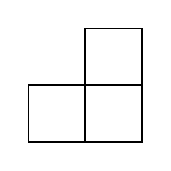
\begin{tikzpicture}[x=.72cm,y=.72cm,line width=.65pt]
\draw (0,0) -- (2,0) -- (2,2) -- (1,2) -- (1,1) -- (0,1) -- cycle;
\draw (1,0) -- (1,1) -- (2,1);
\end{tikzpicture}}\endgroup\par
Три грани в плоской развёртке, без подписей.}
\end{GelfandAdjacentEvidence}
\begin{GelfandAdjacentEvidence}{GELFAND-P000627}{5}

[Справа от рисунка:] обойдём на плоск. замкн. путь
соотв. путь на кубе: придём в другую точку (кручение)
и повернёмся (кривизна).

Неясно, как на многогранниках выглядят основные геом. вещи (\(n\)-мерный случай).
Хар. классы и т.д. [зачёркнуто]
\Incomplete{GELFAND-P000627}{cancelled-geometry}{Короткая запись после «и т.д.» густо зачёркнута.}
\end{GelfandAdjacentEvidence}
\begin{GelfandAdjacentEvidence}{GELFAND-P000627}{6}

\underline{Задача:} сделать общую теор. относительности на решётках.

\underline{Список того, что нужно знать из физики (разумному математику).}

1. Фейнман, Хибс «Кв. мех. и инт. по траекториям».

2. Лекции Фейнмана для школьников.

3. Квантовая механика: Ландау, Лифшиц (теория возмущ., квазиклассич. приближение
[зачёркнуто], группы Ли, осн. понятия по теории рассеяния).
\Unclear{GELFAND-P000627}{landau-short}{После «приближение» зачёркнут знак, похожий на скобку. Запятая видна справа.}
\end{GelfandAdjacentEvidence}
\begin{GelfandAdjacentEvidence}{GELFAND-P000627}{7}


4. Релят. кв. мех. --- начало Берестецкого, Лифшица, Питаевского; вторичное квантование
(кн. Дирака [зачёркнуто]; Фейнман «Стат. механика»).
\Unclear{GELFAND-P000627}{dirac-short}{После «Дирака» зачёркнут знак, похожий на скобку. Точка с запятой видна справа.}
\end{GelfandAdjacentEvidence}


Стат. физика --- Ландау и Лифшиц.


\Needspace{7\baselineskip}
\begin{GelfandAdjacentEvidence}{GELFAND-P000628}{1}
\SourcePage{GELFAND-P000628}{unlabelled}
\underline{Что надо знать из математики физикам?}

1. Предст. групп.

2. Псевдодифф. операторы.

3. Интегр. опер. Фурье--Хёрмандера.

4. \(P^\lambda\) (полиномы Бернштейна).
\[
LP^\lambda=a(\lambda)P^{\lambda-1}.
\]
\Unclear{GELFAND-P000628}{bernstein-coefficient}{Коэффициент в правой части читается \(a(\lambda)\).}
\end{GelfandAdjacentEvidence}
\begin{GelfandAdjacentEvidence}{GELFAND-P000628}{2}


5. Теорема Римана--Роха.

6. Связь особ. с топ. циклов.

\underline{Поляков.}
\Incomplete{GELFAND-P000628}{cancelled-heading}{Под фамилией густо заштрихованная полоса.}
\end{GelfandAdjacentEvidence}
\begin{GelfandAdjacentEvidence}{GELFAND-P000628}{3}

[Справа:] \underline{ТМФ предпосл. номер}; ст. по полю Янга--Миллса --- расписано.

Янг, Миллс --- перев. в сб. «Элем. частицы и компенсир. поля» (1964).
\Unclear{GELFAND-P000628}{yang-citation}{Перед «в сб.» читается сокращение «перев.».}
\end{GelfandAdjacentEvidence}
\begin{GelfandAdjacentEvidence}{GELFAND-P000628}{4}


Есть кварки \(q\simeq\begin{pmatrix}u\\d\\s\end{pmatrix}\).
спин кварка \(\tfrac12\),
\(B\sim\) спин \(\tfrac12\) (барион),
\(M\) --- спин \(0\) (мезон).
\[
\begin{aligned}
M&\sim\overline q q&&\text{(кварк и антикварк)},\\
B&\sim qqq.
\end{aligned}
\]
\underline{Откуда}: Групп. в мультиплеты (по 8 штук).
(идея Гелл-Манна и Неймана).
\Unclear{GELFAND-P000628}{multiplets-word}{После «Групп. в» написано «мультиплеты».}
\end{GelfandAdjacentEvidence}
\begin{GelfandAdjacentEvidence}{GELFAND-P000628}{5}

\Unclear{GELFAND-P000628}{neeman-name}{Вторая фамилия написана «Неймана».}
\end{GelfandAdjacentEvidence}
\begin{GelfandAdjacentEvidence}{GELFAND-P000628}{6}

\(\Rightarrow\) Симметрии: наиболее подх. гр. \(SU(3)\),
предст. \(\underline{8,10,27}\) (разл.).

\underline{Низшие представления?} [зачёркнуто] скалярн., станд. и тенз. произвед.
\Unclear{GELFAND-P000628}{reps-short}{Перед «скалярн.» стоит короткий зачёркнутый знак.}
\end{GelfandAdjacentEvidence}
\begin{GelfandAdjacentEvidence}{GELFAND-P000628}{7}

Пусть это реальные частицы! замеч. идея:
\[
\begin{aligned}
3^*\times3&=1+8,\\
3\times3\times3&=1+8+8+10.
\end{aligned}
\]
\(\Rightarrow\) нельзя стр. мезоны как 3 кварка; их 8, а \(3\times3=3^*+6\).

Рассеиваем:
\[
\frac{\sigma(BB)}{\sigma(BM)}=\frac32
\qquad\text{(сечения)}.
\]
--- так и получается (точн. \(10\%\)).
Большие эн. --- рассеив. [зачёркнуто] частица на частице, как част. на античастице.
\Incomplete{GELFAND-P000628}{scatter-cancelled-word}{Короткое слово перед «частица» густо зачёркнуто.}
\end{GelfandAdjacentEvidence}
\begin{GelfandAdjacentEvidence}{GELFAND-P000628}{8}


\(\underline{qqqq\overline q}\) --- отсутств. в опыте (наз. экзотическими).

Много частиц --- скор. вращ. кварков (как электрон в ат. водорода).
\underline{но}: нестабильны (резонанс). Перех. в основное состояние.
\Unclear{GELFAND-P000628}{rotational-abbrev}{Перед «вращ.» написано «скор.».}
\end{GelfandAdjacentEvidence}
\begin{GelfandAdjacentEvidence}{GELFAND-P000628}{9}


\underline{Волн. ф-я бариона:}
\[
\Delta^{++}\simeq u(x_1)u(x_2)u(x_3),
\]
но нужна антисимм..

Предлаг. 3 сорта и 3 цвета.
\[
q=\begin{array}{@{}c@{\quad}l@{}}
\left(\begin{array}{ccc}
\makebox[12mm]{\(u_{\text{к}}\)}&\makebox[12mm]{\(u_{\text{ж}}\)}&\makebox[12mm]{\(u_{\text{с}}\)}\\
d_{\text{к}}&d_{\text{ж}}&d_{\text{с}}\\
s_{\text{к}}&s_{\text{ж}}&s_{\text{с}}
\end{array}\right)&
\begin{array}{@{}l@{}}
\text{верхние}\\
\text{нижние}\qquad\text{(Гелл-Манн)}\\
\text{странные}
\end{array}\\[-1pt]
\begin{array}{ccc}
\makebox[12mm]{красн.}&\makebox[12mm]{жёлт.}&\makebox[12mm]{синие}
\end{array}&
\end{array}.
\]
\Unclear{GELFAND-P000628}{color-grid}{В матрице написаны индексы «к», «ж», «с». Названия цветов стоят под соответствующими столбцами.}
\end{GelfandAdjacentEvidence}


На опыте кварки не сущ. (\(90\%\)).
\(\mathcal L\) не может быть инвар. отн.
\[
SU(3)\otimes SU_c(3)
\qquad\overset{\nwarrow}{\text{цветная (перемен. цвета)}}.
\]


\Needspace{7\baselineskip}
\begin{GelfandAdjacentEvidence}{GELFAND-P000629}{1}
\SourcePage{GELFAND-P000629}{unlabelled}
Счит., что только бесцв. част. имеют не очень большие массы, цветные --- \(\infty\).
\[
M\sim\overline q_{\text{к}}q_{\text{к}}+
\overline q_{\text{жс}}\overline q_{\text{жс}}+
\overline q_{\text{с}}q_{\text{с}}.
\]
\Unclear{GELFAND-P000629}{meson-index}{В среднем слагаемом над обоими \(q\) стоят черты. Оба индекса предположительно читаются «жс».}
\end{GelfandAdjacentEvidence}
\begin{GelfandAdjacentEvidence}{GELFAND-P000629}{2}

Лагранжиан должен запрещать появл. цветных частиц (должны им беск. массы).
Пусть взаимод. перен. цв. полями Янга--Миллса (глюонами).

\(SU(3)\) --- прибл. симметрия. (\(20\)--\(30\%\)).
Пусть \(SU_c(3)\) --- точная группа.
(Возм., есть 4-й сорт (очарованные), но наверняка есть 3 цвета).

Мезонов (см. ф-лу) должно быть 9. Но их больше. Отсюда необх. 4-й кварк.
(4 года назад). [зачёркнуто]\qquad \(SU(4)\otimes SU_c(3)\).
\Incomplete{GELFAND-P000629}{cancelled-quark-line}{Запись после «4 года назад» густо зачёркнута.}
\end{GelfandAdjacentEvidence}
\begin{GelfandAdjacentEvidence}{GELFAND-P000629}{3}

\[
\mathcal L=\overline q(i\gamma_\mu\nabla_\mu-m)q+
\frac{1}{4e^2}\operatorname{Sp}(F_{\mu\nu}^2).
\]
Есть 8 полей Янга--Миллса. (Глюоны --- от glu --- клей --- склеив. кварки).
Они безмассовые. \underline{8 цветных глюонов}.

Сохр. токи \(\Longleftrightarrow\) наличие симметрии.
Хотим показать, что если гр. неабелева \(\Rightarrow\)
\underline{эн. взаимод. \(\sim\) [зачёркнуто] \(R\)} (расст.)
(\(\Rightarrow\) струна, соед. кварки, не рвётся)
(в абелевой \(\sim R^{-1}\), ур-я Максвелла).
\Unclear{GELFAND-P000629}{cancelled-potential}{Перед \(R\) зачёркнута короткая запись с горизонтальным штрихом.}
\end{GelfandAdjacentEvidence}
\begin{GelfandAdjacentEvidence}{GELFAND-P000629}{4}

\[
\mathcal L=\frac{1}{4e^2}\operatorname{tr}(F_{\mu\nu}^2).
\]
\SourceFigure{GELFAND-P000629}{heavy-charges}{%
\par\smallskip
\begingroup\color{black}\GelfandFitDiagram{\begin{tikzpicture}[x=.74cm,y=.74cm,line width=.55pt]
\filldraw[fill=black!28] (0,1.57) circle (.19);
\filldraw[fill=black!28] (-.025,.56) circle (.21);
\draw (0,1.38) .. controls (.10,1.29) and (-.15,1.25) .. (0,1.19)
 .. controls (.11,1.15) and (-.15,1.08) .. (0,1.02)
 .. controls (.10,.97) and (-.12,.92) .. (0,.88)
 .. controls (.09,.83) and (-.06,.81) .. (-.025,.77);
\node[right,align=left] at (.36,1.07) {\(M\to\infty\)\\2 тяжёлых заряда};
\end{tikzpicture}}\endgroup\par
Два заштрихованных круга соединены волнистой линией.}
\end{GelfandAdjacentEvidence}
\begin{GelfandAdjacentEvidence}{GELFAND-P000629}{5}


\underline{Г. Классич. вар.}: некоммут. электротехника.
\Unclear{GELFAND-P000629}{classical-heading}{Сокращение после «Классич.» предположительно читается «вар.».}
\end{GelfandAdjacentEvidence}
\begin{GelfandAdjacentEvidence}{GELFAND-P000629}{6}

\SourceFigure{GELFAND-P000629}{gluon-exchange}{%
\par\smallskip
\begingroup\color{black}\GelfandFitDiagram{\begin{tikzpicture}[x=.78cm,y=.78cm,line width=.55pt]
\draw (0,1.2) .. controls (.28,.94) and (1.14,.97) .. (1.55,1.15);
\draw (.10,.01) .. controls (.62,.23) and (.97,.16) .. (1.43,-.14);
\draw (.56,1.03)--(.44,.73)--(.62,.66)--(.51,.45)--(.68,.39)--(.64,.23)--(.57,.17);
\draw (1.04,1.01)--(.96,.82)--(1.05,.76)--(1.18,.74)--(1.10,.57)
 .. controls (1.16,.38) and (1.19,.30) .. (1.15,.00);
\draw (1.50,1.09)--(1.23,.60)--(1.13,.52)
 .. controls (1.03,.45) and (.91,.66) .. (.70,.48)--(.60,.42);
\draw (.94,1.01)--(.86,.87)--(.92,.80)--(.77,.64);
\node[right,align=left] at (1.72,.60) {обмен клеем\\(глюонами)};
\end{tikzpicture}}\endgroup\par
Две границы и соединяющие их штрихи. Точные соединения в середине не вполне ясны.}
\end{GelfandAdjacentEvidence}
\begin{GelfandAdjacentEvidence}{GELFAND-P000629}{7}

\SourceFigure{GELFAND-P000629}{pair-creation}{%
\par\smallskip
\begingroup\color{black}\GelfandFitDiagram{\begin{tikzpicture}[x=.78cm,y=.78cm,line width=.55pt]
\draw (0,1.16) .. controls (.35,1.00) and (1.13,1.07) .. (1.48,1.27);
\draw (-.10,.02) .. controls (.49,.39) and (1.07,-.09) .. (1.56,-.11);
\draw (.43,1.08) .. controls (.40,.97) and (.62,1.02) .. (.52,.83);
\draw (.94,1.12) .. controls (.81,.99) and (1.00,.98) .. (.98,.86);
\draw (.47,.77) .. controls (.25,.57) and (.54,.47) .. (.75,.48)
 .. controls (1.10,.48) and (1.23,.72) .. (1.04,.80)
 .. controls (.89,.86) and (.62,.82) .. (.46,.83);
\draw (.48,.50) .. controls (.25,.36) and (.63,.40) .. (.40,.19);
\draw (.96,.53) .. controls (.78,.35) and (1.22,.41) .. (1.13,.24)--(1.06,.17);
\draw[<-] (1.72,.68)--(2.19,.68);
\node[right,align=left] at (2.19,.68) {обр. пары\\\underline{кв.--антикв.}};
\draw[->] (.72,-.29)--(.87,.03);
\node[below,align=center] at (1.70,-.28) {Малый вклад, если \(M\to\infty\)};
\end{tikzpicture}}\endgroup\par
Овал между двумя границами. Стрелки ведут к овалу и к нижней линии.}
\end{GelfandAdjacentEvidence}
\begin{GelfandAdjacentEvidence}{GELFAND-P000629}{8}

\Unclear{GELFAND-P000629}{heavy-note-word}{Первое слово под рисунком переписано и предположительно читается «Малый».}
\end{GelfandAdjacentEvidence}
\begin{GelfandAdjacentEvidence}{GELFAND-P000629}{9}

\[
\begin{aligned}
\frac{\int DA_\mu\,e^{i\int\mathcal L\,d^4x}\,
          \operatorname{tr}e^{i\oint A_\mu\,dx_\mu}}
     {\int DA_\mu\,e^{i\int\mathcal L\,d^4x}}
&=\left\langle\operatorname{tr}e^{i\oint_C A_\mu\,dx_\mu}\right\rangle
=e^{iW(C)}.
\end{aligned}
\]
\Unclear{GELFAND-P000629}{action-dx}{Последний знак после \(d^4\) в числителе переписан и предположительно читается \(x\).}
\end{GelfandAdjacentEvidence}
\begin{GelfandAdjacentEvidence}{GELFAND-P000629}{10}

\Unclear{GELFAND-P000629}{line-integral-dx}{Знак \(x\) после \(d\) в контурном интеграле числителя переписан. Нижнего \(C\) у этого интеграла не видно.}
\end{GelfandAdjacentEvidence}
\begin{GelfandAdjacentEvidence}{GELFAND-P000629}{11}

\SourceFigure{GELFAND-P000629}{ordering-contour}{%
\par\smallskip
\begingroup\color{black}\GelfandFitDiagram{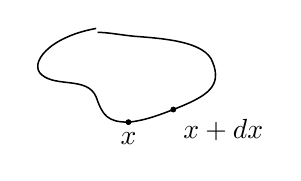
\begin{tikzpicture}[x=1cm,y=1cm,line width=.55pt]
\draw (.79,1.19) .. controls (.18,1.08) and (-.07,.74) .. (.10,.60)
 .. controls (.29,.44) and (.68,.58) .. (.79,.32)
 .. controls (.87,.09) and (.93,.00) .. (1.20,.00)
 .. controls (1.43,.02) and (1.67,.12) .. (1.87,.20)
 .. controls (2.20,.34) and (2.39,.46) .. (2.27,.76)
 .. controls (2.18,1.02) and (1.68,1.06) .. (1.28,1.09)
 .. controls (1.08,1.11) and (.94,1.14) .. (.81,1.14);
\fill (1.20,0) circle (.037) node[below] {\(x\)};
\fill (1.77,.16) circle (.037) node[below right] {\(x+dx\)};
\end{tikzpicture}}\endgroup\par
На контуре отмечены две точки. После \(x+dx\) виден короткий штрих, уверенного индекса нет.}
\end{GelfandAdjacentEvidence}
\begin{GelfandAdjacentEvidence}{GELFAND-P000629}{12}

\[
\operatorname{tr}\prod_x(1+iA_\mu(x)\,dx_\mu)
\]
--- контурный интеграл. (такое упорядочение).
(\(T\) --- экспонента Дайсона).

\underline{Утверждение:}
\SourceFigure{GELFAND-P000629}{long-contour}{%
\par\smallskip
\begingroup\color{black}\GelfandFitDiagram{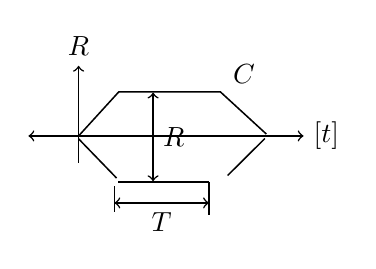
\begin{tikzpicture}[x=.91cm,y=.81cm,line width=.55pt]
\draw[<->] (-.70,0)--(3.14,0) node[right] {\([t]\)};
\draw[->] (0,-.42)--(0,1.10) node[above] {\(R\)};
\draw (0,0)--(.56,.69)--(1.98,.69)--(2.62,.03);
\draw (0,-.045)--(.53,-.66);
\draw (.55,-.72)--(1.82,-.72);
\draw (2.08,-.62)--(2.60,-.04);
\draw[<->] (1.04,-.71)--(1.04,.68) node[midway,right] {\(R\)};
\draw (.50,-.79)--(.50,-1.20);
\draw (1.82,-.72)--(1.82,-1.24);
\draw[<->] (.50,-1.05)--(1.82,-1.05) node[midway,below] {\(T\)};
\node[above] at (2.31,.67) {\(C\)};
\end{tikzpicture}}\endgroup\par
Контур \(C\), ось \(R\) и размеры \(R\) и \(T\). Справа у нижней стороны контура виден разрыв.}
\end{GelfandAdjacentEvidence}
\begin{GelfandAdjacentEvidence}{GELFAND-P000629}{13}

\Unclear{GELFAND-P000629}{graph-label}{Переписанная метка горизонтальной оси предположительно читается \(t\).}
\end{GelfandAdjacentEvidence}

Рассм. такой контур.
Здесь \(W(C)\xrightarrow[T\to\infty]{}E(R)T\), где \(E(R)\)
--- энергия взаимод. зарядов.


\Needspace{7\baselineskip}
\begin{GelfandAdjacentEvidence}{GELFAND-P000630}{1}
\SourcePage{GELFAND-P000630}{unlabelled}
\underline{Объяснение:} если сист. в стац. сост.,
то амплит. перех. за время \(T\): \(F=e^{-iET}\) (\(E\) --- энергия).
\Unclear{GELFAND-P000630}{stationary-phase}{В показателе написано \(-iET\). Над первым \(F\) виден отдельный штрих.}
\end{GelfandAdjacentEvidence}
\begin{GelfandAdjacentEvidence}{GELFAND-P000630}{2}

\underline{С другой стор.}
\[
F=e^{-iET}=\sum_{(\text{пути})} e^{iS}.
\]
\SourceFigure{GELFAND-P000630}{time-path}{%
\par\smallskip
\begingroup\color{black}\GelfandFitDiagram{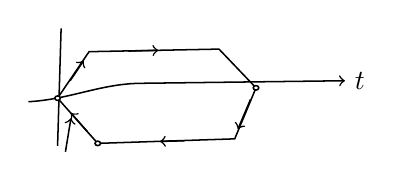
\begin{tikzpicture}[x=1cm,y=.82cm,line width=.55pt]
\draw (0,-.74)--(.045,1.08);
\draw[->] (-.37,-.055) .. controls (.15,-.02) and (.54,.22) .. (1.04,.23)
 -- (3.65,.27) node[right] {\(t\)};
\draw (0,0)--(.40,.72)--(2.05,.76)--(2.52,.16)--(2.25,-.63)
 --(.51,-.70)--cycle;
\draw[->] (.16,.27)--(.33,.58);
\draw[->] (.90,.73)--(1.28,.74);
\draw[->] (2.45,-.02)--(2.29,-.48);
\draw[->] (1.61,-.66)--(1.30,-.67);
\draw[->] (.38,-.52)--(.17,-.23);
\draw[->] (.10,-.83)--(.17,-.31);
\draw[fill=white] (0,0) circle (.035);
\draw[fill=white] (.51,-.70) circle (.035);
\draw[fill=white] (2.52,.16) circle (.035);
\end{tikzpicture}}\endgroup\par
На верхней стороне стрелки направлены вправо, на нижней влево. У начала контура отдельная стрелка снизу.}
\end{GelfandAdjacentEvidence}
\begin{GelfandAdjacentEvidence}{GELFAND-P000630}{3}

[Под рисунком:] созд. пары част.--античаст. (сверхтяж.); держим долго.

Классич. действие \(S=\int_{(x)}^{(x')}A_\mu\,dx_\mu\). В эл.-магн. поле.
Античаст. \(\sim\) част., идущая назад по времени.
Отсюда \(W(C)\sim S_C\) (площ. внутри контура). \(\sim RT\to E\sim R\).
Считается методом перевала.
\Unclear{GELFAND-P000630}{saddle-word}{Последнее слово написано «перевала».}
\end{GelfandAdjacentEvidence}
\begin{GelfandAdjacentEvidence}{GELFAND-P000630}{4}

\[
\int DA_\mu\, e^{i\int(\partial_\mu A_\nu-\partial_\nu A_\mu)^2}
 e^{i\oint A_\mu\,dx_\mu}
=e^{-\oint\!\oint dx\,dx'\,D(x-x')},
\]
где \(D=\dfrac{1}{(x-x')^2+i0}\) (ф-я Грина ур-я Даламбера).
\[
W=\mathrm{const}\cdot T+\frac{e^2T}{R}+\ldots
\]

\underline{След. раз:}
\[
\frac{\int DA\,e^{\frac{1}{4e^2}\int F_{\mu\nu}^{2}}\,
\text{[зачёркнуто]}\cdot\operatorname{tr}e^{\oint A_\mu\,dx_\mu}}{N}
\qquad\text{--- вычислим}.
\]
\Unclear{GELFAND-P000630}{cancelled-exponent-atom}{Перед контурным интегралом зачёркнут короткий знак. Под ним вписано \(\cdot\operatorname{tr}e\).}
\end{GelfandAdjacentEvidence}
\begin{GelfandAdjacentEvidence}{GELFAND-P000630}{5}

негауссов, т.к. в \(F_{\mu\nu}\) есть квадр. член \([A_\mu,A_\nu]\).
\[
F_{\mu\nu}=\partial_\mu A_\nu-\partial_\nu A_\mu+[A_\mu,A_\nu].
\]
(В эл.-магн. поле коммутатор \(0\)).
Эл.-дин. с компактной калибр. группой --- уже возникает неоднозн. экстремалей.
\underline{Кварки в Янге--Миллса не сделана.}
\Unclear{GELFAND-P000630}{closing-word}{Последнее слово читается «сделана».}
\end{GelfandAdjacentEvidence}

\begin{center}\textemdash\,\textperiodcentered\,\textemdash\end{center}


\Needspace{7\baselineskip}
\begin{GelfandAdjacentEvidence}{GELFAND-P000631}{1}
\SourcePage{GELFAND-P000631}{unlabelled}
\underline{9/\(\overline{\underline{\mathrm{II}}}\)-76.}\qquad\underline{Сем. Гельфанда.}
\Unclear{GELFAND-P000631}{date-day}{Цифра дня густо переписана и читается «9».}
\end{GelfandAdjacentEvidence}
\begin{GelfandAdjacentEvidence}{GELFAND-P000631}{2}

\underline{Кричевер.}
\underline{Ур-я Зах.--Шабата.}
\Unclear{GELFAND-P000631}{heading-short}{Окончание сокращения «Ур-я» густо переписано.}
\end{GelfandAdjacentEvidence}
\begin{GelfandAdjacentEvidence}{GELFAND-P000631}{3}

\begin{equation*}
\left[L_1-\frac{\partial}{\partial y},L_2-\frac{\partial}{\partial t}\right]=0,\tag{1}
\end{equation*}
\[
\begin{aligned}
L_1&=\sum_{i=0}^n u_i(x,y,t)\frac{\partial^i}{\partial x^i},\\
L_2&=\sum_{i=0}^m v_i(x,y,t)\frac{\partial^i}{\partial x^i},
\end{aligned}
\qquad
\left.\begin{array}{ll}u_n=1,&u_{n-1}\\v_m=1,&v_{m-1}\end{array}\right\}
=\mathrm{const}.
\]
\Incomplete{GELFAND-P000631}{coeff-cancelled-expression}{После \(u_n\) есть зачёркнутая запись с \(=1\) над ней. Под \(v_m\) вписана \(1\).}
\end{GelfandAdjacentEvidence}
\begin{GelfandAdjacentEvidence}{GELFAND-P000631}{4}


Рассм. форм. ряд
\begin{equation*}
\Psi=e^{kx+k^ny}\left(\sum_{i=0}^{\infty}\xi_i(x,y,t)\frac{1}{k^i}\right),
\qquad \xi_0=1.\tag{2}
\end{equation*}
Пусть \(\left(L-\dfrac{\partial}{\partial y}\right)\Psi=0\), где \(L=L_1\).
Коэфф. рекурр. вычисл.
\begin{equation*}
\sum_{i=0}^n u_i\sum_{\ell=0}^i C_i^\ell\,\xi_{\ell-s}^{(i-\ell)}
=\xi_{n-s}+\frac{\partial}{\partial y}\xi_{-s},
\quad s=n,n-1,\ldots\ \text{до }-\infty.\tag{3}
\end{equation*}
\(\xi_{-s}=0\) при \(s>0\).
\Unclear{GELFAND-P000631}{zero-index-range}{Знак перед \(0\) густо переписан, предположительно \(>\).}
\end{GelfandAdjacentEvidence}
\begin{GelfandAdjacentEvidence}{GELFAND-P000631}{5}

[зачёркнуто] опред. \(\xi'_{n-s}\) \(\Rightarrow\) надо const интегр.
\Incomplete{GELFAND-P000631}{cancelled-before-determined}{Короткое слово перед «опред.» зачёркнуто.}
\end{GelfandAdjacentEvidence}
\begin{GelfandAdjacentEvidence}{GELFAND-P000631}{6}

\Unclear{GELFAND-P000631}{derivative-index}{Индекс у \(\xi'\) предположительно читается \(n-s\).}
\end{GelfandAdjacentEvidence}
\begin{GelfandAdjacentEvidence}{GELFAND-P000631}{7}

\(\xi_0=1,\quad \xi_i(0,y,t)=0\) при \(i>1\) --- нормировка.
\Unclear{GELFAND-P000631}{normalization-bound}{В условии нормировки отчётливо написано \(i>1\).}
\end{GelfandAdjacentEvidence}
\begin{GelfandAdjacentEvidence}{GELFAND-P000631}{8}

Обр., \(\forall\) ряда \(\exists\) оп., где всё вып. с точн. до \(k^{-1}\).

\underline{Алгебраич. оператор.} --- если \(\exists\) анал. прод. по \(1/k\)
на комп. алг. кривую (мером. в доп. к точке, [под строкой: где сущ. особ.]).

\underline{Г.} Ур-е Зах.--Шабата
\[
\frac{\partial K_2}{\partial y}-\frac{\partial K_1}{\partial t}=[K_1,K_2],
\]
\(K_1,K_2\) --- дифф. операторы.
\(K_1,K_2\) --- матр. по \(y\) и \(t\) или опер. по другим переменным.
Есть много путей, прив. к этому ур-ю.
\(y,t\) --- параметры.
[Слева: зачёркнуто]
\Unclear{GELFAND-P000631}{margin-short}{Короткая зачёркнутая запись предположительно читается «На».}
\end{GelfandAdjacentEvidence}

Установим равноправие \(x,y,t\). Тогда записывается в виде (1).

Зад. для школьников: найти опер. вида
\[
-\frac{d^2}{dx^2}+u(x)=L_1,\qquad
\frac{d^3}{dx^3}+v_1\frac{d}{dx}+v_2=L_2,
\]
к-рые коммутируют. Делается через эллипт. ф-и или эллипт. кривые.
Если только \(\dfrac{d^n}{dx^n}\), то
\[
\frac{d^n}{dx^n}\Psi-\frac{\partial\Psi}{\partial y}=0
\quad\Rightarrow\quad\Psi=e^{kx+k^ny}.
\]


\Needspace{7\baselineskip}
\begin{GelfandAdjacentEvidence}{GELFAND-P000632}{1}
\SourcePage{GELFAND-P000632}{unlabelled}
Точнее: метод интегр. опер. Фурье.
\[
e^{kx+k^ny}\left(1+\frac{\xi_1(x,y,t)}{k}+\ldots\right).
\]
\underline{Кр.} Сопост. каждому оп. \(L\) --- форм. ряд (2).
Рекурр. соотн. (3) однозн. восст. с точн. до нормировки.

\underline{Определение.} \(L\) наз. алгебраическим, если форм. ряд (2)
имеет мером. прод. [вставлено: (в доп. к отмеч. точке)]
на комп. алг. кривую, причём полюса не зависят от \(x,y,t\).
\Unclear{GELFAND-P000632}{marked-point-insertion}{Над строкой вписано «в доп. к отмеч. точке».}
\end{GelfandAdjacentEvidence}
\begin{GelfandAdjacentEvidence}{GELFAND-P000632}{2}

\[
L\longrightarrow \text{[зачёркнуто]}\ \mathcal R
\]
\Incomplete{GELFAND-P000632}{curve-cancelled-expression}{После стрелки перед \(\mathcal R\) густо зачёркнута запись.}
\end{GelfandAdjacentEvidence}
\begin{GelfandAdjacentEvidence}{GELFAND-P000632}{3}

\(\mathcal R\) --- алг. кр. с отмеч. точкой \(P_0\) и наб. полюсов
\(D_1+\ldots+D_g\), \(g\) --- род кривой
--- это наз. данные рассеяния для \(L\).
\Unclear{GELFAND-P000632}{polepoints-short}{Первый знак после \(D_1\) переписан и предположительно читается \(+\).}
\end{GelfandAdjacentEvidence}
\begin{GelfandAdjacentEvidence}{GELFAND-P000632}{4}

\(P_0\) --- точка, где сущ. особ..
\(1/k\) --- лок. парам. в окр. \(P_0\).

\underline{Г.} Асимпт. разл. как правило не сходится.
В опр. предполаг. сходимость.
\underline{К.} Алг. оператору \(L\leadsto\) алг. крив. с отмеч. точкой и набор полюсов.
\underline{Г.} \(C^\infty\) --- ф-ла Тейлора асимпт. \(\Rightarrow\) аналит. --- сход..
Аналог квазианалитичности?

\underline{К.} \underline{Т. (Ахиезер)}
\(\forall\) неособ. алг. кривой \(\mathcal R\) с отм. точкой \(P_0\)
и фикс. лок. пар. в окр. \(P_0\) и отм. наб. полюсов
\(\exists\) однозн. опр. с точн. до проп. ф-я \(\Psi(x,y,P)\) с зад. наб. полюсов и
\[
\underbrace{\Psi(x,y,P)e^{-kx-k^ny}}_{1+o(1/k)}
\quad\text{--- рег. в окр. }P_0.
\]
\Unclear{GELFAND-P000632}{little-o}{Под скобкой написано \(1+o(1/k)\), с малой \(o\).}
\end{GelfandAdjacentEvidence}
\begin{GelfandAdjacentEvidence}{GELFAND-P000632}{5}

\SourceFigure{GELFAND-P000632}{rectangle-sketch}{%
\par\smallskip
\begingroup\color{black}\GelfandFitDiagram{\begin{tikzpicture}[x=1cm,y=1cm,line width=.55pt]
\draw (0,0) rectangle (1.55,1.08);
\end{tikzpicture}}\endgroup\par
Прямоугольник без подписей.}
\end{GelfandAdjacentEvidence}
\begin{GelfandAdjacentEvidence}{GELFAND-P000632}{6}

\(e^{\zeta(P)x}\) [стрелка к \(\zeta\):] Вейерштрасса (Камке).

\underline{Д-во:} явная ф-ла (будет предъявлена позже).
\underline{Теор.} Ур-е алгебраично \(\Rightarrow\exists\) ф-я \(\Psi\)
\(\Rightarrow\) мы знаем все \(\xi\)
\(\Rightarrow\) находятся все \(u_i\) (однозн.) --- почему они сущ.?
По [зачёркнуто] \(\Psi\) находятся \(u_i\)!!
\Unclear{GELFAND-P000632}{bottom-short}{Перед \(\Psi\) зачёркнут короткий знак.}
\end{GelfandAdjacentEvidence}
\begin{GelfandAdjacentEvidence}{GELFAND-P000632}{7}

[Внизу справа, зачёркнуто: \(\forall\) ряда \(\exists\) опер.:]
\Incomplete{GELFAND-P000632}{bottom-cancelled-insert}{Под левым концом зачёркнутой строки видна ещё одна короткая зачёркнутая запись.}
\end{GelfandAdjacentEvidence}



\Needspace{7\baselineskip}
\begin{GelfandAdjacentEvidence}{GELFAND-P000633}{1}
\SourcePage{GELFAND-P000633}{unlabelled}
\(\forall\) ряда \(\exists\) опер.:
\[
L\Psi-\frac{\partial}{\partial y}\Psi=
\text{[зачёркнуто]}\left(e^{kx+k^ny}o(1/k)\right).
\]
(первые \(n-2\) ур-я)
\Unclear{GELFAND-P000633}{series-word}{В первой строке написано «ряда».}
\end{GelfandAdjacentEvidence}
\begin{GelfandAdjacentEvidence}{GELFAND-P000633}{2}

\Unclear{GELFAND-P000633}{top-cancel}{Короткая запись после знака равенства густо зачёркнута.}
\end{GelfandAdjacentEvidence}
\begin{GelfandAdjacentEvidence}{GELFAND-P000633}{3}

\Unclear{GELFAND-P000633}{top-o-argument}{Аргумент читается \(1/k\). Перед ним маленькая округлая буква, предположительно \(o\).}
\end{GelfandAdjacentEvidence}
\begin{GelfandAdjacentEvidence}{GELFAND-P000633}{4}


\(L\Psi-\dfrac{\partial\Psi}{\partial y}\)
уд. всем треб. теор. Ахиезера \(\Rightarrow\) она \(\equiv0\).

\underline{Дринфельд.}

\underline{Попытка алгебраизации прошлого докл. Кричевера}

Опис. коммут. подколец в кольце дифф. операторов.

\underline{Г.} Цель --- некомм. закон взаимности.
\Unclear{GELFAND-P000633}{reciprocity}{Перед «закон» написано сокращение «некомм.».}
\end{GelfandAdjacentEvidence}
\begin{GelfandAdjacentEvidence}{GELFAND-P000633}{5}


\(B\) --- [зачёркнуто] комм. кольцо с \(1\), снабж. дифф.
[зачёркнуто] \(b\mapsto b'\) [зачёркнуто].
(\(\mathbb C\)-алгебра)
\Incomplete{GELFAND-P000633}{b-first-cancel}{Запись после \(B\) и тире густо зачёркнута.}
\end{GelfandAdjacentEvidence}
\begin{GelfandAdjacentEvidence}{GELFAND-P000633}{6}

\Unclear{GELFAND-P000633}{b-derivative-cancel}{После «дифф.» зачёркнут короткий знак.}
\end{GelfandAdjacentEvidence}
\begin{GelfandAdjacentEvidence}{GELFAND-P000633}{7}

\Unclear{GELFAND-P000633}{b-prime-cancel}{После \(b'\) зачёркнут короткий знак.}
\end{GelfandAdjacentEvidence}
\begin{GelfandAdjacentEvidence}{GELFAND-P000633}{8}

\[
B[\mathcal D],\qquad
\underbrace{\sum b_i\mathcal D^i}_{\text{многочл.}},\qquad
\underbrace{Db-bD=b'}_{\text{прав. умножения}}.
\]
(\(b'\) --- произв. в \(B\))

\(X\) --- комп. рим. пов. над \(\mathbb C\), \(P\) --- фикс. точка.
Обозначим через \(A\) [зачёркнуто] кольцо мером. ф-й на \(X\) [зачёркнуто]
с полюсом лишь в \(P\).
\Unclear{GELFAND-P000633}{a-after-symbol}{После \(A\) есть густо зачёркнутый знак.}
\end{GelfandAdjacentEvidence}
\begin{GelfandAdjacentEvidence}{GELFAND-P000633}{9}

\Incomplete{GELFAND-P000633}{a-poles-cancel}{Слово после \(X\) густо зачёркнуто.}
\end{GelfandAdjacentEvidence}
\begin{GelfandAdjacentEvidence}{GELFAND-P000633}{10}


Опишем гомоморфизмы \(A\to B[\mathcal D]\).
(на самом деле других комм. подколец не бывает --- теор. Шабата)

\underline{Г.} Реальная зад.: найти все расширения тел Гельфанда--Кириллова.

Полиномиальность мешает.
\[
\sum_{i=0}^{k} b_iD^i,\qquad
\underline{\text{эллиптичность}}:\quad\exists b_k^{-1}.
\]
\underline{Треб.}: образ \(\forall\) ненулев. элем. из \(A\) эллиптичен.

\underline{Ранг.} \(a\ne0,\quad a\in A\).
\[
\left.
\begin{gathered}
\operatorname{ord}(a)\text{ --- порядок образа }a\\
\operatorname{ord}(ab)=\operatorname{ord}(a)+\operatorname{ord}(b)\\
\operatorname{ord}(a+b)\le\text{[зачёркнуто]}\max(\operatorname{ord}(a),\operatorname{ord}(b))\\
\operatorname{ord}\lambda=0\quad\text{при }\lambda\in\mathbb C
\end{gathered}
\right]\quad\underline{\text{нормирование}}.
\]
\Unclear{GELFAND-P000633}{norm-cancel}{После знака неравенства зачёркнута запись, предположительно \(\operatorname{ord}(a)+\operatorname{ord}(b)\).}
\end{GelfandAdjacentEvidence}

\(\operatorname{deg}a\) --- порядок полюса \(a\) в точке \(P\).

\underline{Тогда} \(\underline{\operatorname{ord}(a)=n\operatorname{deg}(a)}\).
(на многочленах --- ясно)

\(n\) --- ранг гомоморфизма.

\underline{Кричевер} --- \(n=1\) (вз. простота порядков опер.).
\par\smallskip\noindent\textemdash\,\textperiodcentered\,\textemdash\par
\(M=B[\mathcal D]\), на \(M\) есть структ. \(B\)-модуля;
\(\varphi:A\to B[\mathcal D]\).


\Needspace{7\baselineskip}
\begin{GelfandAdjacentEvidence}{GELFAND-P000634}{1}
\SourcePage{GELFAND-P000634}{unlabelled}
\(M_n\) --- опер. порядка \(\le n\).

[зачёркнуто: Это \(B\)-подмодуль.]
\Unclear{GELFAND-P000634}{top-cancel}{Зачёркнутая строка предположительно читается «Это \(B\)-подмодуль».}
\end{GelfandAdjacentEvidence}
\begin{GelfandAdjacentEvidence}{GELFAND-P000634}{2}


\(M\) --- это \(A\otimes B\)-модуль, т.е.
\(A\)-модуль и \(B\)-модуль и умн. на
\(A\) и \(B\) коммутируют.
\[
\begin{aligned}
bx&=bx \quad\text{(умн. слева)},\\
ax&=x\varphi(a),\\
a\in A&\Rightarrow aM_i\subset M_{i+\operatorname{deg}a\cdot n}.
\end{aligned}
\]
\(\nabla:M\to M\) --- умн. слева на \(D\).
\[
\nabla(x)=Dx.
\]
\(\nabla\) коммут. с действ. \(A\), а \(\nabla b-b\nabla=b'\).

\underline{Обр.} если есть \(A\otimes B\)-мод. \(M\)
с фильтр. и всеми этими соотн., то \(\exists\) гомом. \(\varphi:A\to B[\mathcal D]\)
ранга \(n\).

Можно забыть о \(\varphi\) и рассм. зад. об \(A\otimes B\)-модулях.

\(\rightarrow\) Итак, \(M\) --- модуль над \(A\otimes B\),
снабж. [зачёркнуто] фильтрацией
\[
0=M_{-1}\subset M_0\subset M_1\subset M_2\subset\cdots
\]
\Incomplete{GELFAND-P000634}{filtration-cancel}{Короткая запись перед «фильтрацией» зачёркнута.}
\end{GelfandAdjacentEvidence}
\begin{GelfandAdjacentEvidence}{GELFAND-P000634}{3}

[Под \(A\): мером. ф-и на \(X\) с ед. полюсом.
Под \(B\): кольцо (\(\mathbb C\)-алг.) с дифф. \(b\mapsto b'\).]
и оператором \(\nabla:M\to M\), причём

\noindent 1) \(\nabla a=a\nabla\).

\noindent 2) \(\nabla b-b\nabla=b'\).

\noindent 3) \(\nabla(M_i)\subset M_{i+1}\),
\(\nabla:M_i/M_{i-1}\overset{\sim}{\to} M_{i+1}/M_i\)
при \(i\geqslant0\).
\Unclear{GELFAND-P000634}{condition-three-bound}{Под знаком \(>\) стоит отдельная наклонная черта. Читается \(i\geqslant0\).}
\end{GelfandAdjacentEvidence}
\begin{GelfandAdjacentEvidence}{GELFAND-P000634}{4}


\noindent 4) \(bM_i\subset M_i\), \(M_i/M_{i-1}\) [зачёркнуто]
своб. \(B\)-модуль с 1-й образующей.
\Unclear{GELFAND-P000634}{condition-four-cancel}{Перед «своб.» зачёркнут знак, похожий на стрелку.}
\end{GelfandAdjacentEvidence}
\begin{GelfandAdjacentEvidence}{GELFAND-P000634}{5}


\noindent 5) \(aM_i\subset M_{i+n\operatorname{deg}a}\),
\[
a:M_i/M_{i-1}\overset{\sim}{\to}
M_{i+n\operatorname{deg}a}/M_{i+n\operatorname{deg}a-1}
\qquad\text{при }i\geqslant0.
\]
\Unclear{GELFAND-P000634}{condition-five-bound}{В пункте 5 повторён знак с отдельной чертой. Читается \(i\geqslant0\).}
\end{GelfandAdjacentEvidence}


\(\sim\) зад. пучка над \(X\otimes B\) с нек-рыми фильтрациями.

\(\nabla\sim\) связность с особ. на \(\infty\).
\begin{center}\textemdash\,\textperiodcentered\,\textemdash\end{center}


\Needspace{7\baselineskip}
\begin{GelfandAdjacentEvidence}{GELFAND-P000635}{1}
\SourcePage{GELFAND-P000635}{unlabelled}
\underline{23/\(\overline{\underline{\mathrm{II}}}\)-76.}\qquad\underline{Сем. Гельфанда.}

\underline{С. П. Новиков} о раб. М. Бродского. (Минск)

\underline{Нек-рые случаи явно решаемых зад., не связ. с KdV}.

\underline{Зад. о колеб. упругого шара.}
\[
-\frac{d^2y}{dr^2}+
\left(\lambda^2f^2(r)-\frac{\ell(\ell+1)}{r^2}\right)y
=\lambda_{k,\ell}y.
\]
\Unclear{GELFAND-P000635}{elastic-equation}{Справа написано \(\lambda_{k,\ell}y\). В скобках перед дробью виден минус.}
\end{GelfandAdjacentEvidence}
\begin{GelfandAdjacentEvidence}{GELFAND-P000635}{2}

Обр. зад. --- восст. пар. упр. среды по набору частот \(\lambda_{k,\ell}\).
Задача переопред. Выясн., когда реш. и как.

Пусть \(rf(r)=u(r)\) монотонная ф-я.

Рассм.
\[
m(\tau)=\int_{H(\tau)}^1
\left(\tau^{-2}f^2(r)-\frac1{r^2}\right)^{1/2}dr
\qquad\text{(прав. квант. Бора)}.
\]
(\(H(\tau)\) --- нуль подкор. выражения)

Рассм.
\[
\tau^*_{k\ell}=\frac{\sqrt{\ell(\ell+1)}}{\lambda_{k\ell}},\qquad
m_{k\ell}=\frac{k+\tfrac14+C}{\sqrt{\ell(\ell+1)}}.
\]
\(\tau^*(m_{k\ell})=\tau^*_{k\ell}\) уст. вз.-однозн. соотв.

\(m_{k\ell}\) всюду плотно;
необх. усл. --- \(\tau_{k\ell}\) плотно.

\[
(rf(r))^{-1}=\psi(\eta).\qquad \tau(m)\longleftrightarrow m(\tau)
\]
\Unclear{GELFAND-P000635}{tau-correspondence}{Между выражениями нарисована стрелка с утолщёнными концами.}
\end{GelfandAdjacentEvidence}
\begin{GelfandAdjacentEvidence}{GELFAND-P000635}{3}

\[
\psi(\eta)=\exp\Bigl(2\int^{1}(\tau^2-\eta^2)^{-1/2}
\frac{d(\tau m(\tau))}{d\tau}\,d\tau
\]
\Unclear{GELFAND-P000635}{inverse-integral}{Верхний предел интеграла написан 1. Нижнего предела и правой скобки не видно.}
\end{GelfandAdjacentEvidence}
\begin{GelfandAdjacentEvidence}{GELFAND-P000635}{4}

Большие \(\ell\) --- квазиклассика.

\underline{Фукс.} Есть мн-зие триангул.
\SourceFigure{GELFAND-P000635}{triangulation}{%
\par\smallskip
\begingroup\color{black}\GelfandFitDiagram{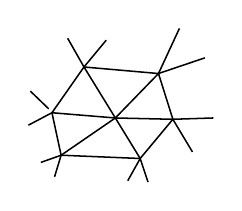
\begin{tikzpicture}[scale=.83,line width=.55pt]
\coordinate (a) at (-.91,.10);
\coordinate (b) at (-.42,.80);
\coordinate (c) at (.72,.70);
\coordinate (d) at (.94,.00);
\coordinate (e) at (.44,-.60);
\coordinate (f) at (-.77,-.55);
\coordinate (o) at (.06,.02);
\draw (a)--(b)--(c)--(d)--(e)--(f)--cycle;
\draw (-1.27,-.09)--(a)--(o)--(d)--(1.56,.02);
\draw (-.67,1.24)--(b)--(o)--(e)--(.56,-.96);
\draw (1.04,1.39)--(c)--(o)--(f)--(-.87,-.88);
\draw (b)--(-.08,1.21);
\draw (c)--(1.43,.94);
\draw (d)--(1.24,-.50);
\draw (e)--(.25,-.94);
\draw (f)--(-1.08,-.66);
\draw (-1.24,.43)--(-.96,.16);
\end{tikzpicture}}\endgroup\par
Сетка треугольников с продолжениями рёбер по краям.}
\end{GelfandAdjacentEvidence}
\begin{GelfandAdjacentEvidence}{GELFAND-P000635}{5}

Рассм. \(\sum\) всех симпл. 1-й разм. с коэфф. \(1\bmod2\). Она не цикл.

У 1-го барицентр. подразделения \(0\).
\SourceFigure{GELFAND-P000635}{barycentric}{%
\par\smallskip
\begingroup\color{black}\GelfandFitDiagram{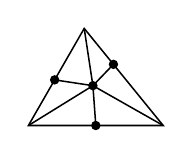
\begin{tikzpicture}[scale=.92,line width=.55pt]
\coordinate (a) at (-.91,0);
\coordinate (b) at (.95,0);
\coordinate (c) at (-.14,1.34);
\coordinate (d) at (-.5481,.6298);
\coordinate (e) at (.2633,.8442);
\coordinate (f) at (.02,0);
\coordinate (o) at (-.02,.55);
\draw (a)--(c)--(b)--cycle;
\draw (a)--(o)--(e) (b)--(o)--(d) (c)--(o)--(f);
\fill (d) circle (.065) (e) circle (.065) (f) circle (.065) (o) circle (.065);
\end{tikzpicture}}\endgroup\par
Треугольник с тремя внутренними линиями и четырьмя отмеченными точками.}
\end{GelfandAdjacentEvidence}
\begin{GelfandAdjacentEvidence}{GELFAND-P000635}{6}

\underline{все центры}, \(\underline{0\bmod2}\) (чётное).

\underline{Штиф. класс --- ему двойственен по Пуанкаре}.
\Unclear{GELFAND-P000635}{stiefel-word}{Написано «Штиф. класс».}
\end{GelfandAdjacentEvidence}

\[
\sum\text{ числа }
\underset{\bmod 2}{=}
\sum(-1)^i\text{ чисел }=\text{эйл. хар.}.
\]

\underline{Лосик (Марк)}.

\underline{Связность.} \(E\to X\) векторное расслоение со слоем \(\mathbb R^n\);
\(p:P\to X\) ассоц. главное расслоение.

\(x\in X\), \(E_x\) --- слой \(E\) в т. \(x\).

\(P_x\ni z\), \(z=(e_{i,x})\), \(i=1,\ldots,n\),
\(z\) --- базис в \(E_x\).

Рассмотрим \(G=GL(n,\mathbb R)\) и определим её действие на \(P\).
\[
A\in G\rightsquigarrow R_A:P\to P,\qquad
R_A(z)=zA=\left(\sum_{j=1}^{n}e_{j,x}A_i^j\right),
\quad A=(A_i^j),\quad i,j=1,\ldots,n.
\]
Это действие гладкое.


\Needspace{7\baselineskip}
\begin{GelfandAdjacentEvidence}{GELFAND-P000636}{1}
\SourcePage{GELFAND-P000636}{unlabelled}
\noindent 1. \((zA)B=z(AB)\).

\noindent 2. \(G\) сохр. слои и действ. просто транзитивно.

\(z\in P_x\), \(V_z\) --- вертик. кас. пр-во (\(\subset T_zP\)).
\(V_z=T_z(P_x)\).

опред. отобр. \(\ell_z:G\to P_x\), \(\ell_z(A)=zA\)

и индуц. отобр. \(\alpha_z:T_e(G)=\mathfrak g\to V_z\) (изоморфизм).
\Unclear{GELFAND-P000636}{tangent-identification}{В записи \(T_e(G)=\mathfrak g\to V_z\) начертание \(\mathfrak g\) наложено на штрихи знака равенства и стрелки.}
\end{GelfandAdjacentEvidence}
\begin{GelfandAdjacentEvidence}{GELFAND-P000636}{2}


\(\beta_z=\alpha_z^{-1}:V_z\to\mathfrak g\)
(лин. форма на \(V_z\) со знач. в \(\mathfrak g\)).

\underline{Связность на гл. расслоении} --- \(1\)-форма на \(P\) со знач. в \(\mathfrak g\), такая, что

\noindent 1. \(\omega|_{V_z}=\beta_z\),

\noindent 2. \(R_A^*\omega=\operatorname{ad}A^{-1}\omega\) (усл. инвариантности).

Для кас. рассл. --- аффинная связность.

Рассм. ур-е \(\omega=0\) в т. \(z\),
\[
H_z=\{\xi\in T_zP:\omega(\xi)=0\}.
\]
\(H_z\) наз. горизонтальным пр-вом.
\(T_z=H_z\oplus V_z\).
\(H_z\) сохр. при действии \(G\).

\begin{center}\textemdash\,\textperiodcentered\,\textemdash\end{center}

Будет постр. рассл., сечения к-рого нах. во вз.-одн. соотв. со связн. на \(P\).

Рассмотрим \(T_z^*\otimes\mathfrak g\) --- \(1\)-формы в т. \(z\) со знач. в \(\mathfrak g\).

Опр. \(\Theta_z\subset T_z^*\otimes\mathfrak g\) как подпр. тех \(\Theta_z\), такая, что
\(\theta_z|_{V_z}=0\).
\Unclear{GELFAND-P000636}{theta-letter}{После «тех» знак похож на прописную \(\Theta_z\). В условии ограничения читается строчная \(\theta_z\).}
\end{GelfandAdjacentEvidence}
\begin{GelfandAdjacentEvidence}{GELFAND-P000636}{3}


\[
\begin{aligned}
C_z&\subset T_z^*\otimes\mathfrak g,\qquad C_z\ni\omega_z:\omega_z|_{V_z}=\beta_z.\\
C_z-C_z&\subset\Theta_z,\qquad
\omega_{1,z}-\omega_{2,z}\in\Theta_z,\qquad
\omega_z+\Theta_z\in C_z.
\end{aligned}
\]
\Unclear{GELFAND-P000636}{affine-membership}{Перед \(C_z\) в последнем соотношении читается знак \(\in\).}
\end{GelfandAdjacentEvidence}


т.е. \(C_z\) --- плоскость, паралл. \(\Theta_z\), но не прох. через \(0\).

Получается рассл. из аффинных пр-в
(«разн. \(2\)-х симв. Кристоффеля --- тензор»).

Над \(P\) рассм. рассл. со слоем \(T_z^*\otimes\mathfrak g\).

Есть отображения:
\[
\widetilde r_{z,A}:T_z^*\otimes\mathfrak g\to T_{zA}^*\otimes\mathfrak g,
\]
индуцир. отображением
\(R_{A^{-1}}^*:T_z^*\to T_{zA}^*\) и
\(\operatorname{ad}A^{-1}:\mathfrak g\to\mathfrak g\).
[Справа: Тенз. произведение отображений.]


\Needspace{7\baselineskip}
\begin{GelfandAdjacentEvidence}{GELFAND-P000637}{1}
\SourcePage{GELFAND-P000637}{unlabelled}
\(C_z\) перех. в соотв. плоск. в т. \(zA\) при этом отобр..

\[
C(P)=\bigcup_{z\in P}C_z
\]
--- естеств. гладкое рассл. над \(P\).

\(G\) действует на \(C(P)\).

[Зачёркнуто: \(C\)?] Инвариантные сечения \(\longleftrightarrow\) связности.
\Unclear{GELFAND-P000637}{first-cancel}{Зачёркнутая запись перед «Инвариантные» начинается знаком, похожим на \(C\).}
\end{GelfandAdjacentEvidence}
\begin{GelfandAdjacentEvidence}{GELFAND-P000637}{2}


\underline{\(C(P)/G=B(P)\)}, [вставлено и обведено «расслоение», со стрелкой к \(\pi\)]
\(\pi:B(P)\to X\).
\Incomplete{GELFAND-P000637}{quotient-cancel}{Слова под обведённым «расслоение» густо зачёркнуты.}
\end{GelfandAdjacentEvidence}
\begin{GelfandAdjacentEvidence}{GELFAND-P000637}{3}


\(C(P)\) --- главное рассл. с базой \(P\), там есть кан. связность.

\underline{Габриэлов.}
[Зачёркнуто: Связность \(\gamma\)? задаёт изоморфизм
\(T^*X\otimes\mathfrak g\to B(P)\).]
\Unclear{GELFAND-P000637}{gabrielov-symbol}{Зачёркнутый знак после «Связность» похож на \(\gamma\).}
\end{GelfandAdjacentEvidence}
\begin{GelfandAdjacentEvidence}{GELFAND-P000637}{4}


(на \(\forall\) слое --- афф. преобразование)

\(1\) св. выбр. \(\to\) другая св. опр. преобр. исх. пр-ва.

(\(\Longleftrightarrow\) разн. связностей --- тензор)

\SourceFigure{GELFAND-P000637}{two-fiber-sketch}{%
\par\smallskip
\begingroup\color{black}\GelfandFitDiagram{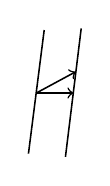
\begin{tikzpicture}[line width=.56pt]
\draw (-.23,0)--(-.03,1.57);
\draw (.24,-.04)--(.44,1.59);
\draw[->] (-.13,.77)--(.34,.77);
\draw[->] (-.13,.77)--(.37,1.04);
\end{tikzpicture}}\endgroup\par
На полях две наклонные линии и две стрелки вправо.}
\end{GelfandAdjacentEvidence}


\par\noindent\begin{minipage}{\linewidth}
\[
\lambda\in T_xX\rightsquigarrow E_x\to E_x
\]
т.е. форма со знач. в гомом.

\underline{\(T^*X\otimes\operatorname{Hom}(E,E)\)}.

\begin{center}\textemdash\,\textperiodcentered\,\textemdash\end{center}
\end{minipage}\par


\Needspace{7\baselineskip}
\begin{GelfandAdjacentEvidence}{GELFAND-P000638}{1}
\SourcePage{GELFAND-P000638}{unlabelled}
\underline{1/III-76.}\quad \underline{Сем. Гельфанда.}
\SourceFigure{GELFAND-P000638}{heading-ornament}{%
\par\smallskip
\begingroup\color{black}\GelfandFitDiagram{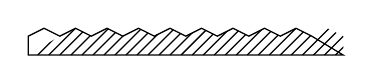
\begin{tikzpicture}[line width=.45pt]
\begin{scope}
\clip (0,0)--(4,0)--(4,.24)
  \foreach \x in {3.8,3.4,...,0.2} {--(\x,.34)--(\x-.2,.24)} --cycle;
\foreach \x in {-.3,-.16,...,4} {\draw (\x,0)--++(.34,.34);}
\end{scope}
\draw (0,.24) \foreach \x in {.2,.6,...,3.8} {--(\x,.34)--(\x+.2,.24)}
  --(4,0)--(0,0)--cycle;
\end{tikzpicture}}\endgroup\par
Штрихованная полоска под заголовком, с волнистым верхним краем.}
\end{GelfandAdjacentEvidence}
\begin{GelfandAdjacentEvidence}{GELFAND-P000638}{2}


\underline{Дринфельд.} (Володя).

\(\overline X\) --- гл. проект. кривая над \(\mathbb C\),
\(P\) --- фикс. точка на \(X\),

\(A\sim\) кольцо рац. ф-й на \(X\) с полюсом в \(P\)
(рег. в \(X\setminus P\)).
\Incomplete{GELFAND-P000638}{first-cancel}{Отдельное слово под определением кольца закрыто плотной штриховкой.}
\end{GelfandAdjacentEvidence}
\begin{GelfandAdjacentEvidence}{GELFAND-P000638}{3}


\underline{Г. Пример.} \(y^2=x(x-1)(x-2)\) (эллиптическая кривая).
\[
P=\infty,\qquad A=\mathbb C[x,y]/(y^2-x(x-1)(x-2)).
\]
\Unclear{GELFAND-P000638}{field-overwrite}{В первом частном знак поля переписан. Предположительно \(\mathbb C\).}
\end{GelfandAdjacentEvidence}
\begin{GelfandAdjacentEvidence}{GELFAND-P000638}{4}


\underline{Ф-и с полюсом 1-го порядка нет.} --- т.к.
[зачёркнуто] \underline{это тор}.
\Incomplete{GELFAND-P000638}{torus-cancel}{Короткое слово между «т.к.» и «это тор» густо зачёркнуто.}
\end{GelfandAdjacentEvidence}
\begin{GelfandAdjacentEvidence}{GELFAND-P000638}{5}


двоякопер.
\Unclear{GELFAND-P000638}{period-abbreviation}{Сокращение читается «двоякопер.».}
\end{GelfandAdjacentEvidence}
\begin{GelfandAdjacentEvidence}{GELFAND-P000638}{6}

\SourceFigure{GELFAND-P000638}{torus-contour}{%
\par\smallskip
\begingroup\color{black}\GelfandFitDiagram{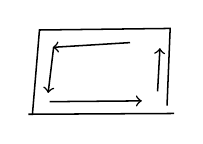
\begin{tikzpicture}[line width=.55pt]
\draw (0,0)--(.09,1.08)--(1.75,1.10)--(1.71,.12);
\draw (-.05,.01)--(1.80,.02);
\draw[->] (1.24,.92)--(.26,.86);
\draw[->] (.27,.86)--(.20,.28);
\draw[->] (.22,.17)--(1.39,.18);
\draw[->] (1.59,.30)--(1.62,.85);
\end{tikzpicture}}\endgroup\par
{\color{black}\(\underline{\int=0}\),\quad \underline{вычет \(=0\)}.}\par\smallskip
Четыре стрелки идут по контуру против часовой стрелки.}
\end{GelfandAdjacentEvidence}
\begin{GelfandAdjacentEvidence}{GELFAND-P000638}{7}


Полюс 2-го пор. --- \(\wp\)-ф-я Вейерштрасса.
(см. Гурвиц, Курант).

[зачёркнуто] \(y^2=x(x-1)\) рода 0 --- \underline{подст. Эйлера}.
\Incomplete{GELFAND-P000638}{genus-zero-cancel}{Короткое слово перед уравнением густо зачёркнуто.}
\end{GelfandAdjacentEvidence}
\begin{GelfandAdjacentEvidence}{GELFAND-P000638}{8}


\(A\) для крив. рода 0 --- многочлены, обр. \(z\).

\underline{\(A\) для элл. кривой} ---
\(\mathbb C[x,y]/(y^2-(x(x-1)(x-2))\).
\Unclear{GELFAND-P000638}{quotient-parenthesis}{В рукописи после произведения отсутствует ещё одна закрывающая скобка.}
\end{GelfandAdjacentEvidence}


\(x\) им. полюс 2-го пор.; перех. в ф-ю Вейерштрасса \(x=\wp(z)\),

\(y\) \textemdash\,\textquotedbl\,\textemdash\ 3-го пор. \(y=\wp'(z)\).

Кольцо \(A\) однозн. опр. кривую и точку.

Как опис. эти кольца?

\begin{center}\textemdash\,\textperiodcentered\,\textemdash\end{center}

\underline{Кричевер.}

почти \(\forall\) точки \(P\) наим. пор. полюса \(\underline{g+1}\).

\underline{Иногда можно ниже} --- в точках Вейерштрасса.

\[
y^2=\prod_{i=1}^{2g+1}(z-z_i)
\]
(гиперэллипт. кривая) --- в т. ветвления есть ф-я с полюсом 2-го порядка.

\(n\) --- мин. возм. кр. полюса в т. \(P\) \(\Rightarrow\) есть полюсы кр. \(2n,3n,\ldots\).

Пусть \(\mu_s\) такие, что \(\underline{\mu_s n+s}\) ---
кратность полюса, \(s=1,\ldots,n-1\).

(\(\mu_s\) --- наименьшие).

Тогда \(\underline{\mu_1+\cdots+\mu_{n-1}=g}\).
\quad \(\Vert\) среди них все образ. (теор. Вейерштрасса).


\Needspace{7\baselineskip}
\begin{GelfandAdjacentEvidence}{GELFAND-P000639}{1}
\SourcePage{GELFAND-P000639}{unlabelled}
\(P\) общ. полож. --- кольцо \(A\) имеет \(g\) образующих ---
с полюсами \(\underline{g+1,g+2,\ldots,2g+1}\) \underline{порядка}.
\Unclear{GELFAND-P000639}{generators-count}{Перед «образующих» читается \(g\). Рядом перечислены порядки от \(g+1\) до \(2g+1\).}
\end{GelfandAdjacentEvidence}
\begin{GelfandAdjacentEvidence}{GELFAND-P000639}{2}


\(B\) --- алгебра над \(\mathbb C\) с дифференцированием \(\mathcal D\).

Есть кольцо \(B[\mathcal D]=\{\sum b_iD^i\}\),
\(\mathcal Db-b\mathcal D=b'\).

Элем. наз. эллипт., если старш. коэфф. обратим.

Опишем гом. \(A\to B[\mathcal D]\), что образ \(\forall\) элем. эллиптичен.

Ранг такого гомоморфизма --- число (нат.) \(n\), такое, что
\[
\forall a\in A,\quad \operatorname{ord}\varphi(a)=n\cdot\operatorname{deg}a.
\]
\(\operatorname{deg}a\) --- пор. полюса \(a\) [зачёркнуто] в т. \(P\).
\Incomplete{GELFAND-P000639}{degree-cancel}{Запись после \(a\) закрыта густым зачёркиванием.}
\end{GelfandAdjacentEvidence}
\begin{GelfandAdjacentEvidence}{GELFAND-P000639}{3}


(\underline{Г.} Есть дифф. опер. 2-го и 3-го пор., коммутир. между собой.)

[зачёркнуто: \(M\)?] гомом. \(\longleftrightarrow\) модули с доп. структурами.
\Unclear{GELFAND-P000639}{module-cancel}{Зачёркнутый знак похож на \(M\).}
\end{GelfandAdjacentEvidence}
\begin{GelfandAdjacentEvidence}{GELFAND-P000639}{4}


\underline{Теор. Кричевера.}

Старший коэффициент гомоморфизма \(\varphi:A\to B[\mathcal D]\).

Пусть \(z\) --- лок. координата в т. \(P\).
Пусть \(a=z^{-k}+\cdots\) (Лорана).

[зачёркнуто: Стар?] \(\varphi(a)=b^k D^{nk}+\cdots\),
\Unclear{GELFAND-P000639}{leading-cancel}{Зачёркнутая запись предположительно читается «Стар».}
\end{GelfandAdjacentEvidence}
\begin{GelfandAdjacentEvidence}{GELFAND-P000639}{5}


где \(\underset{\substack{\uparrow\\ B}}{b}\) не зависит от \(k\)
и от выбора лок. параметра.

(сущ. полюса \(\forall\) пор., начиная с нек-рого; надо делить)

\underline{\(b\) наз. старшим коэфф. гомоморфизма \(\varphi\)}.

\underline{опр.} [зачёркнуто: Это?] \(\varphi_1\sim\varphi_2\),
если \(\exists b\in B^*\),
\(\underline{\varphi_1(a)=b\varphi_2(a)b^{-1}}\).
\Unclear{GELFAND-P000639}{equivalence-cancel}{Зачёркнутая запись над началом определения предположительно читается «Это».}
\end{GelfandAdjacentEvidence}
\begin{GelfandAdjacentEvidence}{GELFAND-P000639}{6}


\(\dfrac{d}{dx}\sim\dfrac{b'}{b}+\dfrac{d}{dx}\).
В ростках \(b'/b\) --- любая ф-я.

\underline{Теор. Кричевера.}
\(B\) [зачёркнуто] --- ростки гладких ф-й на прямой.
\Incomplete{GELFAND-P000639}{germs-formula-cancel}{Формула после \(B\) перечёркнута. Видны скобки, чтение не установлено.}
\end{GelfandAdjacentEvidence}


гомом. \(\varphi\) ранга \(1\) (с точн. до эквив!)
\(\longleftrightarrow\) старший коэфф. и точка на якобиане кривой
(якобиево многообразие), \(J_X\).

\underline{С. Гельф.}
\underline{1-мерные вект. рассл. степени \(0\)}
(\(\sim\) дивизор с точн. до эквивал.)
\[
\begin{array}{l@{\qquad}l}
Q_1,\ldots,Q_\ell & \\
n_1,\ldots,n_\ell & \text{степень } n_1+\cdots+n_\ell=0.\\
\multicolumn{1}{c}{\text{целые}} &
\end{array}
\]

\underline{эквивалентность}: если отлич. на дивизор ф-и (мероморфной).

\underline{Эквив.} --- рассл. зад. глоб. мером. сечениями.


\Needspace{7\baselineskip}
\begin{GelfandAdjacentEvidence}{GELFAND-P000640}{1}
\SourcePage{GELFAND-P000640}{unlabelled}
\underline{Г. Аналит. опред. якобиева мн-зия:} на \(\overline X\) сущ. дифф. 1-го рода
(без особ.) их \(g\) штук.

\(y^2=x(x-a)(x-b)\),

\(\Vert\dfrac{dx}{y}\) не имеет особ.
(в т. \(x=0,a,b\) нет, т.к. \(x\) не лок. парам.).

\SourceFigure{GELFAND-P000640}{abel-paths}{%
\par\smallskip
\begingroup\color{black}\GelfandFitDiagram{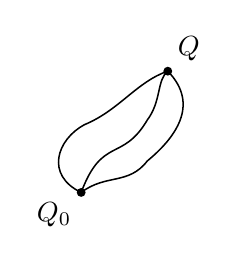
\begin{tikzpicture}[line width=.55pt]
\coordinate (q0) at (0,0);
\coordinate (q) at (1.10,1.54);
\draw (q0).. controls (-.46,.22) and (-.31,.67)..(.04,.86)
  .. controls (.48,1.04) and (.71,1.41)..(q);
\draw (q0).. controls (.27,.72) and (.52,.38)..(.84,.92)
  .. controls (1.02,1.16) and (.96,1.43)..(q);
\draw (q0).. controls (.32,.24) and (.60,.09)..(.84,.40)
  .. controls (1.18,.68) and (1.52,1.11)..(q);
\fill (q0) circle (1.6pt) node[below left] {\(Q_0\)};
\fill (q) circle (1.6pt) node[above right] {\(Q\)};
\end{tikzpicture}}\endgroup\par
Три пути между \(Q_0\) и \(Q\).}
\end{GelfandAdjacentEvidence}
\begin{GelfandAdjacentEvidence}{GELFAND-P000640}{2}


\(z_i=\int_{Q_0}^{Q}\omega_i\). [зачёркнуто: Это?]
(\(\int\) по кл. гомологий; базис --- \(g\) чисел)
\Unclear{GELFAND-P000640}{integral-cancel}{Зачёркнутая запись после интеграла, предположительно «Это».}
\end{GelfandAdjacentEvidence}
\begin{GelfandAdjacentEvidence}{GELFAND-P000640}{3}


форма опр. наб. инт. по периодам.

с точн. до периодов --- \(\mathbb C^g/\underline{\text{решётка}}\).
\quad \(n_1\alpha_1+\cdots+n_{2g}\alpha_{2g}\).

Не все торы получаются.

Дивизор --- лин. комб. точек; точки тора можно склад..

\SourceFigure{GELFAND-P000640}{divisor-motion}{%
\par\smallskip
\begingroup\color{black}\GelfandFitDiagram{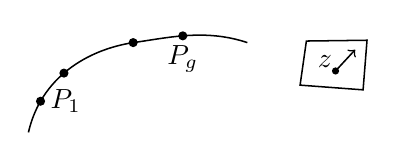
\begin{tikzpicture}[line width=.55pt]
\draw (0,0).. controls (.16,.70) and (.75,1.05)..(1.33,1.14)
  coordinate[pos=.21] (p1) coordinate[pos=.46] (p2) coordinate (p3)
  .. controls (1.77,1.20) and (2.24,1.32)..(2.78,1.14)
  coordinate[pos=.46] (pg);
\fill (p1) circle (1.65pt) node[right] {\(P_1\)};
\fill (p2) circle (1.65pt);
\fill (p3) circle (1.65pt);
\fill (pg) circle (1.65pt) node[below] {\(P_g\)};
\draw (3.45,.60)--(3.53,1.16)--(4.30,1.17)--(4.25,.54)--cycle;
\fill (3.90,.78) circle (1.3pt) node[above left,inner sep=1pt] {\(z\)};
\draw[->] (3.90,.78)--(4.15,1.05);
\end{tikzpicture}}\endgroup\par
Точки на кривой и стрелка от \(z\) в прямоугольнике.}
\end{GelfandAdjacentEvidence}
\begin{GelfandAdjacentEvidence}{GELFAND-P000640}{4}


движ. по прямой на торе \(\to\) движ. \(P_1,\ldots,P_g\) [зачёркнуто] по кривой.
\Incomplete{GELFAND-P000640}{motion-cancel}{Слово между \(P_g\) и «по кривой» густо зачёркнуто.}
\end{GelfandAdjacentEvidence}
\begin{GelfandAdjacentEvidence}{GELFAND-P000640}{5}


\begin{center}\textemdash\,\textperiodcentered\,\textemdash\end{center}

Зад. гом. из \(A\) в кольцо \(B[\mathcal D]\) экв. зад. следующего.

\(M\) --- модуль над \(A\otimes B\),
\(\nabla:M\to M\), \(\nabla(am)=a\nabla(m)\),
\(\nabla(bm)=b\nabla(m)+b'm\).

\[
0=M_{-1}\subset M_0\subset M_1\subset M_2\subset\cdots,\qquad
\dim_B M_i/M_{i+1}=1\quad\text{при }i\geqslant0.
\]
\Unclear{GELFAND-P000640}{reverse-quotient}{У размерности в рукописи стоит \(M_i/M_{i+1}\).}
\end{GelfandAdjacentEvidence}
\begin{GelfandAdjacentEvidence}{GELFAND-P000640}{6}

\[
\begin{aligned}
BM_i&\subset M_i,\\
\nabla M_i&\subset M_{i+1},\qquad
\nabla_*:M_i/M_{i-1}\overset{\sim}{\to}M_{i+1}/M_i,\\
aM_i&\subset M_{i+\operatorname{deg}a},\\
a:M_i/M_{i-1}&\overset{\sim}{\to}M_{i+\operatorname{deg}a}/M_{i+\operatorname{deg}a-1}.
\end{aligned}
\]

\begin{center}\textemdash\end{center}

\underline{\(\varphi:A\to B[\mathcal D]\)}, \(\Rightarrow B[\mathcal D]=M\).
[зачёркнуто: \(A\otimes B\)-модуль?]
\Unclear{GELFAND-P000640}{module-phrase-cancel}{В зачёркнутой строке предположительно читается \(A\otimes B\)-модуль.}
\end{GelfandAdjacentEvidence}
\begin{GelfandAdjacentEvidence}{GELFAND-P000640}{7}


Умн. на \(B\) слева и на \(A\) справа,
\[
\begin{array}{rcl}
ma &=& m\varphi(a).\\[-.4ex]
   & \scriptstyle\mathrm{def} & \\[-.6ex]
bm &=& bm.
\end{array}
\]
\Unclear{GELFAND-P000640}{def-placement}{Помета \(\mathrm{def}\) стоит между двумя знаками равенства.}
\end{GelfandAdjacentEvidence}
\begin{GelfandAdjacentEvidence}{GELFAND-P000640}{8}


\(\nabla:M\to M\) умн. на \(\mathcal D\) слева.

\underline{Фильтр. --- порядок}.

\underline{посл. усл.} --- эллиптичность.

\begin{center}\textemdash\,\textperiodcentered\,\textemdash\end{center}

Как по \(M\) построить \(\varphi\)?

[зачёркнуто: \(M\)?] \(M_{-1}=0\),
\Unclear{GELFAND-P000640}{m-cancel}{Зачёркнутый знак похож на \(M\).}
\end{GelfandAdjacentEvidence}
\begin{GelfandAdjacentEvidence}{GELFAND-P000640}{9}

\(\nabla:M_0\overset{\sim}{\to}M_1/M_0\).
в \(M_0\) есть образующая \(e\) (над \(B\)).

положим \(D=\nabla(e)\).

\(\varphi(a)\) ясно, т.к. есть \(A\)-модуль и т.д..

\begin{center}\textemdash\,\textperiodcentered\,\textemdash\end{center}

\underline{След. шаг:} перев. на язык пучков.

[зачёркнуто: на кривой] \(M_{-1}=0\subset M_0\subset M_1\subset\cdots\)
\Unclear{GELFAND-P000640}{curve-cancel}{Зачёркнутая надпись «на кривой» перед фильтрацией.}
\end{GelfandAdjacentEvidence}
\begin{GelfandAdjacentEvidence}{GELFAND-P000640}{10}


\(\sim\) вект. рассл. [вставлено: 1-мерное] на \(X\)
с равными \(0\) когом. (0-мерн. и 1-мерн.) пучка сечений.

[Справа]
\[
aM_i\subset M_{i+\operatorname{deg}a},\qquad
a:M_i/M_{i-1}\overset{\sim}{\to}M_{i+\operatorname{deg}a-1}
\quad(i\geqslant0).
\]
\Unclear{GELFAND-P000640}{margin-graded}{В правой записи у стрелки выписан один член фильтрации.}
\end{GelfandAdjacentEvidence}



\Needspace{7\baselineskip}
\begin{GelfandAdjacentEvidence}{GELFAND-P000641}{1}
\SourcePage{GELFAND-P000641}{unlabelled}
\SourceFigure{GELFAND-P000641}{top-margin-mark}{%
\par\smallskip
\begingroup\color{black}\GelfandFitDiagram{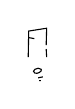
\begin{tikzpicture}[line width=.4pt,scale=.6]
\draw (0,.38)--(.01,.93)--(.39,.99)--(.38,.63) (.38,.55)--(.39,.38);
\draw (.02,.79)--(.13,.77);
\draw (.28,.12).. controls (.19,.19) and (.05,.08)..(.14,.04)
  .. controls (.20,.02) and (.29,.07)..(.28,.12);
\draw (.21,-.06)--(.31,-.04) (.23,-.12)--(.27,-.12);
\end{tikzpicture}}\endgroup\par
В правом верхнем поле метка из трёх сторон и несколько отдельных штрихов под ней.}
\end{GelfandAdjacentEvidence}
\begin{GelfandAdjacentEvidence}{GELFAND-P000641}{2}


\(L\) --- 1-мерное вект. расслоение над \(\overline X\),
\(H^0(X,\underline L)=H^1(X,\underline L)=0\).

(\(H^0(X,\underline L)=0\) и \(\operatorname{deg}L=g-1\)).

\(M=H^0(X-P,\underline L)\) (алгебраические сеч.,
голом. с ед. полюсом).
\Unclear{GELFAND-P000641}{holomorphic-abbrev}{Сокращение после «алгебраические сеч.» читается «голом.».}
\end{GelfandAdjacentEvidence}
\begin{GelfandAdjacentEvidence}{GELFAND-P000641}{3}


\(M_i\) [зачёркнуто: \(-\)?] с полюсом порядка \(i+1\).
\Unclear{GELFAND-P000641}{m-i-cancel}{После \(M_i\) зачёркнут короткий горизонтальный знак.}
\end{GelfandAdjacentEvidence}
\begin{GelfandAdjacentEvidence}{GELFAND-P000641}{4}


\(M_{-1}=0\) --- 1-е условие, (\(H^0=0\)).

\[
\dim M_i/M_{i-1}=1,\qquad
M_0=H^0(X,\underset{\substack{\uparrow\\\text{с полюсом в }P}}{\underline L(P)}).
\]
\[
0\to\underline L\to\underline L(P)\to\underline L(P)/\underline L\to0.
\]
точн. посл. когом. \(\Rightarrow\dim_{\mathbb C}M_i/M_{i-1}=1\).

\begin{center}\shortstack{\textemdash\\[-.35em]\textemdash}\end{center}

Обр. есть послед. модулей, постр. пучок
\[
0=M_{-1}\subset M_0\subset M_1\subset M_2\subset\cdots,\qquad
\dim_{\mathbb C}M_i/M_{i-1}=1.
\]
\(M\) --- модуль над \(A\).

\[
\begin{aligned}
aM_i&\subset M_{i+\operatorname{deg}a}\\
a_*:M_i/M_{i-1}&\overset{\sim}{\to}
M_{i+\operatorname{deg}a}/M_{i+\operatorname{deg}a-1},\qquad i\geqslant0.
\end{aligned}
\]
\Unclear{GELFAND-P000641}{graded-symbol}{Индекс при \(a\) в обозначении отображения похож на звёздочку.}
\end{GelfandAdjacentEvidence}
\begin{GelfandAdjacentEvidence}{GELFAND-P000641}{5}


\underline{Сеч. пучка зададим над откр. мн-вами по Зарискому}.

Пучок квазикогерентный; дост. зад. на откр. афф. подмн-вах.

\(a_0\in A\), \(a_0\ne\mathrm{const}\) \(\Vert\) покрытие
\[
X=(X\setminus P)\cup(X\setminus\text{нули }a_0).
\]
Сеч. над \(X\setminus P\), \(A\)-модуль --- \(M\).

Над \(X\setminus\text{нули }a_0\) --- \(m/a_0^k\),
\(m\in M_{k\cdot\operatorname{deg}a_0-1}\).

\underline{След. раз:} Дринфельд \(20\) мин., Шнирельман.
\Incomplete{GELFAND-P000641}{bottom-clipped}{Ниже последней строки различимы только отдельные верхние штрихи.}
\end{GelfandAdjacentEvidence}



\Needspace{7\baselineskip}
\begin{GelfandAdjacentEvidence}{GELFAND-P000642}{1}
\SourcePage{GELFAND-P000642}{unlabelled}
\noindent\textperiodcentered\hfill\textemdash\,\textperiodcentered\,\textemdash\par
\underline{15/III-76 г.}\quad \underline{Сем. Гельфанда.}\quad \underline{Дринфельд.}

\(\overline X\) --- гладкая проект. кривая над \(\mathbb C\)

\(P\in\overline X\),

\(A\in H^0(X-P,\mathcal O_X)\) --- рац. ф-и на \(\overline X\) с полюсом в \(P\).
\Unclear{GELFAND-P000642}{ring-membership}{Между \(A\) и \(H^0\) стоит знак \(\in\).}
\end{GelfandAdjacentEvidence}
\begin{GelfandAdjacentEvidence}{GELFAND-P000642}{2}


\(B\) --- алгебра над \(\mathbb C\) (с диффер. [ниже: обозн.?]),
\(z\) --- лок. коорд. на \(\overline X\) в окр. \(P\).
\Unclear{GELFAND-P000642}{derivation-insertion}{Под «с диффер.» написано сокращение, похожее на «обозн.», и два коротких штриха.}
\end{GelfandAdjacentEvidence}
\begin{GelfandAdjacentEvidence}{GELFAND-P000642}{3}


Ищутся гомоморфизмы \(\varphi:A\to B[\mathcal D]\) ранга \(1\),

т.е. \(\forall a\in A\), \(a=z^{-m}+\cdots\Rightarrow\varphi(a)=b^mD^m+\cdots\)

\(b\) --- старший коэффициент \(\varphi\).

Они рассм. с точн. до сопряжения обрат. элементами из \(B\).

[зачёркнуто: \(B\)?] Задание \(\varphi\) равносильно тогда заданию
\(A\otimes B\)-модуля \(M\)
\Unclear{GELFAND-P000642}{assignment-cancel}{Перед «Задание» зачёркнут знак, похожий на \(B\).}
\end{GelfandAdjacentEvidence}
\begin{GelfandAdjacentEvidence}{GELFAND-P000642}{4}


[зачёркнуто: е?] и отображения \(\nabla:M\to M\), таких что
\Unclear{GELFAND-P000642}{first-cancel}{Короткий зачёркнутый знак перед «и отображения» похож на «е».}
\end{GelfandAdjacentEvidence}
\begin{GelfandAdjacentEvidence}{GELFAND-P000642}{5}


\(\nabla(am)=a\nabla(m)\), [зачёркнуто: и?]
\(\nabla(bm)=b\nabla(m)+b'm\),
\(\underset{\text{(фильтрация)}}{M=\bigcup M_i}\),
\Unclear{GELFAND-P000642}{am-cancel}{Между формулами для отображения зачёркнут знак, похожий на «и».}
\end{GelfandAdjacentEvidence}
\begin{GelfandAdjacentEvidence}{GELFAND-P000642}{6}


\(BM_i\subset M_i\), [зачёркнуто: \(BM_i\)?]
\(M_{-1}=0\), \(M_i/M_{i-1}=B\) при \(i\geqslant0\).
\Unclear{GELFAND-P000642}{bm-cancel}{Зачёркнутая запись похожа на \(BM_i\).}
\end{GelfandAdjacentEvidence}


\[
\begin{gathered}
\forall a\in A,\qquad aM_i\subset M_{i+\operatorname{deg}a},\\
a:M_i/M_{i-1}\overset{\sim}{\to}M_{i+\operatorname{deg}a}/M_{i+\operatorname{deg}a-1},\\
\nabla:M_i/M_{i-1}\overset{\sim}{\to}M_{i+1}/M_i,\qquad i\geqslant0.
\end{gathered}
\]

\underline{Г. следствие:} \(\exists\) опер., все степени к-рого, кроме \(1\)-й ---
дифф. операторы (\(2\)-я, \(3\)-я и т.д.).

\(\overline X\) --- алг. кр. рода \(g\), \(P\) --- точка.

\(n\) --- мин. возм. кратность полюса в т. \(P\) (единств. полюса).

\(\mu_i\) --- наим. числа, для к-рых сущ. полюс кр. \(i+\mu_i n\), \(i=1,\ldots,n-1\).

Тогда \(\sum\mu_i=g\).


\Needspace{7\baselineskip}
\begin{GelfandAdjacentEvidence}{GELFAND-P000643}{1}
\SourcePage{GELFAND-P000643}{unlabelled}
[зачёркнуто: Сущ. ф…?]
\Unclear{GELFAND-P000643}{cancel-top}{Начало зачёркнутой строки предположительно «Сущ. ф…».}
\end{GelfandAdjacentEvidence}
\begin{GelfandAdjacentEvidence}{GELFAND-P000643}{2}

(Пропущено \(g\) кратностей полюсов\({}^*\))

[Стрелка от звёздочки] это [зачёркнуто] и обратно влечёт утв., сформ. Кричевером.
\Incomplete{GELFAND-P000643}{cancel-top-right}{После «это» слово закрыто густым зачёркиванием.}
\end{GelfandAdjacentEvidence}
\begin{GelfandAdjacentEvidence}{GELFAND-P000643}{3}


\underline{Д. На язык пучков.}

Всё, кроме \(\nabla\), \(\sim\) зад. вект. рассл. \(L\) на \(\overline X\),
для к-рого \(H^0(X,\underline L)=H^1(X,\underline L)=0\).

\(\sim\) зад. 1-мерн. рассл. \(L\) над \(X\otimes B\),
\[
H^0(X\otimes B,\underline L)=H^1(X\otimes B,\underline L)=0.
\]
\[
X=U_1\cup\cdots\cup U_k,\qquad U_i=\operatorname{Spec}R_i.
\]
Склеим афф. схемы \(\operatorname{Spec}\) [зачёркнуто] \(R_i\otimes B\).
\Incomplete{GELFAND-P000643}{cancel-affine}{Между Spec и выражением справа густо зачёркнуты знаки.}
\end{GelfandAdjacentEvidence}
\begin{GelfandAdjacentEvidence}{GELFAND-P000643}{4}


\underline{Интуитивно:} росток гладк. сем-ва вект. расслоений.

\[
\nabla:\underline L\longrightarrow
\underset{\substack{\nearrow\\\text{с особ. 1-го пор. в т. }P}}{\underline L(P)}
\qquad
\underline L\longrightarrow\underline L(P)/\underline L\longrightarrow0.
\]
[Справа] \(H^0(\underline L(P)/\underline L)\) свободно
(огранич. на т. \(P\) тривиально).

\(\nabla b-b\nabla=b'\), \(\nabla\) --- \(O_X\)-линейно.

\underline{Старш. коэфф.} --- ?

Тривиализуем в окр. \(P\), Пусть \(e\) --- базис.
\[
\frac{\nabla(e)}{e}=\frac{1}{b_0z}+\cdots
\quad\Rightarrow\quad b_0\text{ --- Старш. коэфф.}.
\]

\underline{Теор. Кричевера.}
Гомом. ранга \(1\) с точн. до сопр. обр. элементами из \(B\)
\(\Longleftrightarrow\) точка на якобиане \(\overline X\) в общем положении.

\noindent 1. Задано \(\varphi\). \(\Rightarrow\) зад. 1-мерн. рассл. над \(X\otimes B\).
Строим точку на якобиане.

Пусть \(\mathbb C\leftarrow B\) и соотв. вложение
\(\overline X\subset X\otimes B\), т.к. есть естеств. отобр. \(B\to\mathbb C\)
(значение в \(0\)).

Ограничиваем \(L\) на \(\overline X\), т.е. получ. вект. рассл. на \(\overline X\).

\noindent 2. Пусть заданы \(L_0\) --- рассл. над \(\overline X\) и задано \(B\).
Построим всё остальное.

\(J\) --- якобиан \(\overline X\), его точки --- векторн. рассл. одинак. степени.

Кас. пр-во к якоб. \(\cong H^1(X,O_X)\)
(сам якобиан \(H^1(X,O_X^*)\).
\(\Rightarrow\) кас. пр-во получ., если убрать \(*\)).

Рассм. точн. послед.
\[
0\longrightarrow O_X\longrightarrow O_X(P)
\longrightarrow O_X(P)/O_X\longrightarrow0.
\]
\Unclear{GELFAND-P000643}{sequence-overwrite}{Буква в начале третьего члена обведена. Предположительно \(O_X(P)/O_X\).}
\end{GelfandAdjacentEvidence}
\begin{GelfandAdjacentEvidence}{GELFAND-P000643}{5}

\Incomplete{GELFAND-P000643}{cancel-sequence}{Под третьим членом последовательности видна зачёркнутая запись.}
\end{GelfandAdjacentEvidence}
\begin{GelfandAdjacentEvidence}{GELFAND-P000643}{6}

[Стрелка вверх] пучок над точкой.

Рассм.
\[
\frac{1}{[\text{зачёркнуто}]z}\in H^0(O_X(P)/O_X)
\xrightarrow[\text{когран. гом.}]{} H^1(X,O_X).
\]
\Incomplete{GELFAND-P000643}{bottom-coefficient}{Знак перед \(z\) в знаменателе залит чернилами.}
\end{GelfandAdjacentEvidence}

(\(z\) --- лок. параметр).

Образ \(1/z\) в кас. пр-во к якобиану обозн. \(\eta_P\in H^1(X,O_X)\).


\Needspace{7\baselineskip}
\begin{GelfandAdjacentEvidence}{GELFAND-P000644}{1}
\SourcePage{GELFAND-P000644}{unlabelled}
\(\ell_0\) --- соотв. точка в якобиане. При изм. \(x\) получаем гл. путь на якобиане
(т. якобиана со знач. в \(B\)).
\[
\underline{\ell'(x)=\frac{\eta_P}{b_0(x)}}
\]
(прямая с изм. параметром).
\Unclear{GELFAND-P000644}{top-point-letter}{Петлевой знак в обеих записях похож на \(\ell\) или \(e\).}
\end{GelfandAdjacentEvidence}
\begin{GelfandAdjacentEvidence}{GELFAND-P000644}{2}


\underline{Снова:} кривая \(X\), точка \(P\), лок. парам..

\(\Rightarrow\) прямая в кас. пр-ве к якобиану.

\(x\in\overline X\) [зачёркнуто] \(x\mapsto\overline{x-P}\) --- \underline{дивизор}.
\Incomplete{GELFAND-P000644}{cancel-divisor}{После принадлежности зачёркнута группа знаков с петлями.}
\end{GelfandAdjacentEvidence}
\begin{GelfandAdjacentEvidence}{GELFAND-P000644}{3}


Получ. отобр. \(\overline X\) в якобиан \(J\).

Кривая им. в т. \(P\) кас. пр-во.
Образ --- 1-мерн. пр-во кас. к якобиану.

\begin{center}\textemdash\,\textperiodcentered\,\textemdash\end{center}

\underline{А. Поляков.}\quad\underline{Калибровочные поля.}\quad\underline{Квантование ур-ий Янга-Миллса.}

Лагранжиан
\[
S=\int\mathcal L(x)d^4x,\qquad \mathcal L(x)=\frac14\operatorname{tr} F_{\mu\nu}^2.
\]
Для гр. \(\mathrm{SU}(2)\) будет \(F_{\mu\nu}\) --- элем. алгебры Ли.
\[
F_{\mu\nu}=\partial_\mu A_\nu-\partial_\nu A_\mu+g[A_\mu,A_\nu].
\]
[Вне правой линии поля]
\Unclear{GELFAND-P000644}{outer-edge-fragment}{Одиночный знак похож на «э» или «3».}
\end{GelfandAdjacentEvidence}
\begin{GelfandAdjacentEvidence}{GELFAND-P000644}{4}


\(A_\mu\), \(\mu=0,1,2,3\) --- антиэрмитовы со следом \(0\) (\(2\times2\)) («бесследная»).

Поля \(A_\mu\) --- дин. переменные.

Эл. поля --- ф-и \(A_\mu(x)\), \(\mu=0,1,2,3\).
\[
A_\mu(x)\in\mathrm{SU}(2)\quad\text{(алг. Ли)}.
\]
\Unclear{GELFAND-P000644}{group-symbol}{В строке написано \(SU(2)\), далее в скобках «алг. Ли».}
\end{GelfandAdjacentEvidence}
\begin{GelfandAdjacentEvidence}{GELFAND-P000644}{5}

\[
F_{\mu\nu}^2=\sum_{\mu,\nu}F_{\mu\nu}F_{\mu\nu}.
\]
\Incomplete{GELFAND-P000644}{cancel-middle}{Справа от суммы зачёркнуто несколько знаков.}
\end{GelfandAdjacentEvidence}
\begin{GelfandAdjacentEvidence}{GELFAND-P000644}{6}


\(A_\mu\) наз. вект. потенциалом,

\(F_{\mu\nu}\) \textemdash\,\textquotedbl\,\textemdash\ тенз. напр. поля.

\underline{Переход к гамильт. формализму.}\quad \(n=1,2,3\).
\[
L=\int\mathcal Ld^3\vec x=\operatorname{tr}\int
\left.\frac12(\dot A_n-\nabla_n A_0)^2-\frac12h_n^2\right\}d^3\vec x
\]
(выделяем время)
\Unclear{GELFAND-P000644}{lagrangian-opening}{В рукописи видна закрывающая фигурная скобка. После знака интеграла открывающей скобки не видно.}
\end{GelfandAdjacentEvidence}


Здесь \(\nabla_n A_0=\partial_n A_0+g[A_n,A_0]\)
(и называем ков. производной).
\[
\begin{aligned}
h_n&=\frac12\varepsilon_{nm\ell}(\partial_m A_\ell-\partial_\ell A_m+g[A_m,A_\ell]),\\
F_{0n}&=\partial_0 A_n-\partial_n A_0+g[A_0,A_n].
\end{aligned}
\]
\[
\underline{\nabla_\mu X\underset{\mathrm{def}}{=}\partial_\mu X+g[A_\mu,X]}.
\]


\Needspace{7\baselineskip}
\begin{GelfandAdjacentEvidence}{GELFAND-P000645}{1}
\SourcePage{GELFAND-P000645}{unlabelled}
\(L\) не сод. \(\dot A_0\),
\(e_n=\dfrac{\partial\mathcal L}{\partial\dot A_n}=\dot A_n-\nabla_n A_0\)
--- \underline{кан. импульс}.

Гамильтониан.
\[
\underline{\mathcal H=e_n\dot A_n-\mathcal L}
=\frac12 e_n(e_n+\nabla_n A_0)+\frac12 h_n^2.
\]
\Unclear{GELFAND-P000645}{legendre-factor}{Перед \(e_n(e_n+\nabla_n A_0)\) в рукописи стоит \(\tfrac12\).}
\end{GelfandAdjacentEvidence}
\begin{GelfandAdjacentEvidence}{GELFAND-P000645}{2}

\[
H=\frac12\int d^3\vec x\,\operatorname{tr}[e_n^2+h_n^2-A_0\nabla_n e_n].
\]
\Unclear{GELFAND-P000645}{gauss-factor}{Множитель перед интегралом читается как половина.}
\end{GelfandAdjacentEvidence}
\begin{GelfandAdjacentEvidence}{GELFAND-P000645}{3}

\Unclear{GELFAND-P000645}{gauss-term}{Перед \(A_0\nabla_n e_n\) написан минус, без отдельного числового множителя.}
\end{GelfandAdjacentEvidence}
\begin{GelfandAdjacentEvidence}{GELFAND-P000645}{4}

\[
-\frac{\delta H}{\delta A_0}=\dot e_0=0.
\]

Ур. Гамильт. \(\leftrightarrow\) ур-я Лагранжа.

Отсюда наложим усл.
\[
\nabla_n e_n=0\tag{*}
\]
\[
\widehat H=\frac12\int d^3\vec x\,[e_n^2+h_n^2].
\]
\SourceFigure{GELFAND-P000645}{canonical-variables}{%
\par\smallskip
\begingroup\color{black}\GelfandFitDiagram{\begin{tikzpicture}[line width=.45pt]
\draw (3.6,1.6)--(.06,1.6)--(0,0)--(3.6,0);
\draw (.16,1.56)--(.10,.09) (.14,.06)--(3.37,.035);
\node[anchor=west,inner sep=2pt] at (.28,1.30) {\(e\) --- импульс};
\node[anchor=west,inner sep=2pt] at (.28,.84) {\(A\) --- координаты};
\node[anchor=west,inner sep=2pt] at (.28,.34) {\(h^2(A)\) --- потенциал};
\end{tikzpicture}}\endgroup\par
Запись в правом поле с незамкнутой рамкой.}
\end{GelfandAdjacentEvidence}
\begin{GelfandAdjacentEvidence}{GELFAND-P000645}{5}


Будет ли вып. в след. момент усл. \((*)\)?

Обозн. \(\nabla_n e_n=\rho(\vec x)\).

Это условие \(\{\rho(x),H\}=0\), где
\[
\{A,B\}=\int d^3\vec x\sum_n
\left(\frac{\delta A}{\delta e_n}\cdot\frac{\delta B}{\delta A_n}
-\frac{\delta A}{\delta A_n}\frac{\delta B}{\delta e_n}\right).
\]
\[
\begin{cases}
\dot A_n=\dfrac{\delta H}{\delta e_n},\\
\dot e_n=-\dfrac{\delta H}{\delta A_n},\\
\nabla_n e_n=0.
\end{cases}
\]

[Справа] \underline{Эти ур-я \(\sim\) ур-ям Лагранжа. Это обобщ. обычного рез.}.

(обобщ. ур-ий Максвелла с \(U(1)\) на любую [зачёркнуто]
компактную группу --- и даже полупростую).
\Incomplete{GELFAND-P000645}{cancel-group}{Между «любую» и «компактную» зачёркнуто слово. Видны нижние петли.}
\end{GelfandAdjacentEvidence}
\begin{GelfandAdjacentEvidence}{GELFAND-P000645}{6}


\begin{center}\textemdash\,\textperiodcentered\,\textemdash\end{center}

\(\exists\) комб. полей Я.-М., от к-рой не зависит потенц. энергия \(h^2\).
\[
\begin{aligned}
h_n&=\frac12\varepsilon_{nm\ell}F_{m\ell},\\
F_{m\ell}&=\partial_m A_\ell-\partial_\ell A_m+g[A_m,A_\ell].
\end{aligned}
\]
\[
\widetilde A_n(x)=\Omega^+A_n\Omega+\frac1g\Omega^+\partial_n\Omega(\vec x),
\]
\(\Omega(x)\) --- произв. матрица, \(\Omega(x)\in SU(2)\).

\(\underline{\widetilde h_n=\Omega^+h_n\Omega}\) --- \underline{прямо проверяется}.

\(\Rightarrow\) потенц. эн. [зачёркнуто] инвар.
(\(\operatorname{Sp}h^2\) не мен.).
\Incomplete{GELFAND-P000645}{cancel-energy}{Перед «инвар.» небольшая запись густо зачёркнута.}
\end{GelfandAdjacentEvidence}


Введ. поле \(a_n\). рассм. поля с усл. \(\underline{\partial_n a_n=0}\).

Положим
\[
\begin{cases}
A_n(x)=\Omega^+(x)a_n\Omega(x)+\dfrac1g\Omega^+\partial_n\Omega(x),\\
\partial_n a_n=0.
\end{cases}
\]
[Справа] \(\Vert\) новый набор переменных.


\Needspace{7\baselineskip}
\begin{GelfandAdjacentEvidence}{GELFAND-P000646}{1}
\SourcePage{GELFAND-P000646}{unlabelled}
\underline{Кан. импульс разб. на 2 части}.
\(P_n\), \(\rho(x)\), \(\partial_nP_n=0\).
\[
e_n=P_n+\partial_n\Psi,\qquad
H=\frac12\int(P_n^2+h_n^2(a)+(\partial_n\Psi)^2)d^3\vec x.
\]
Для нах. \(\Psi\) использ. то, что \(\nabla_n e_n\underset{\mathrm{def}}{=}\rho(\vec x)\).
\[
\begin{aligned}
\nabla_nP_n+\nabla_n\partial_n\Psi&=\rho,\\
\nabla_n\partial_n\Psi&=\rho+[P_n,a_n].
\end{aligned}
\]
\Unclear{GELFAND-P000646}{charge-commutator-first}{В первой формуле записано \([P_n,a_n]\) без множителя \(g\).}
\end{GelfandAdjacentEvidence}
\begin{GelfandAdjacentEvidence}{GELFAND-P000646}{2}

\((\partial_n\Psi)^2\) наз. \underline{кулоновской энергией}.

\begin{center}\textemdash\,\textperiodcentered\,\textemdash\end{center}

\[
\begin{aligned}
H&=\int(e_n^2+h_n^2(A)),\\
A_n&\longrightarrow\Omega^+a_n\Omega+\Omega^+\partial_n\Omega,\\
\partial_n a_n&=0.
\end{aligned}
\]
\[
\begin{cases}
H=\int(P_n^2+(\partial_n\Psi)^2+h^2),\\
\nabla_n\partial_n\Psi=[a_n,P_n].
\end{cases}
\qquad\text{(швингер)}
\]
\Unclear{GELFAND-P000646}{schwinger-note}{Справа в скобках читается «швингер».}
\end{GelfandAdjacentEvidence}
\begin{GelfandAdjacentEvidence}{GELFAND-P000646}{3}

\Unclear{GELFAND-P000646}{charge-commutator-second}{В этом месте порядок в скобках \([a_n,P_n]\).}
\end{GelfandAdjacentEvidence}
\begin{GelfandAdjacentEvidence}{GELFAND-P000646}{4}


Здесь \(h_n(a)=\frac12\varepsilon_{nm\ell}(\partial_m a_\ell-\partial_\ell a_m+g[a_m,a_\ell])\).
\(\Psi\) нах. из посл. ур-я.

\[
\nabla_n e_n=\rho(\vec x)\quad\Rightarrow\quad
\left\{\begin{aligned}
\partial^2\Psi&=\rho(x)\quad\text{(в скал. случае)},\\
\int(\partial\Psi)^2dx&=\int\frac{\rho(x)\rho(y)}{|x-y|}\,dx\,dy.
\end{aligned}\right.
\]
--- кулон. взаимод..
\Unclear{GELFAND-P000646}{scalar-abbrev}{Над равенством читается «в скал. случае».}
\end{GelfandAdjacentEvidence}
\begin{GelfandAdjacentEvidence}{GELFAND-P000646}{5}

\SourceFigure{GELFAND-P000646}{coulomb-callout}{%
\par\smallskip
\begingroup\color{black}\GelfandFitDiagram{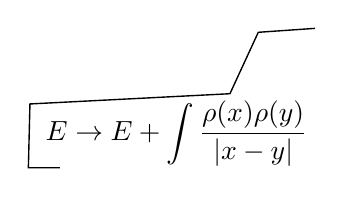
\begin{tikzpicture}[line width=.5pt]
\draw (.4,0)--(0,0)--(.02,.81)--(2.56,.94)--(2.92,1.72)--(3.64,1.77);
\node[anchor=west,inner sep=2pt] at (.14,.43)
  {\(\displaystyle E\to E+\int\frac{\rho(x)\rho(y)}{|x-y|}\)};
\end{tikzpicture}}\endgroup\par
Ломаная линия соединяет запись энергии с предыдущими формулами.}
\end{GelfandAdjacentEvidence}
\begin{GelfandAdjacentEvidence}{GELFAND-P000646}{6}


\underline{Неаб. случай}. Сначала по теории возмущ. (сначала Хриплович, потом Гросс и т.д.).

\underline{Классич. случай:} \(g=0\Rightarrow\) зад. абелева.

Получ.
\[
\partial^2\Psi+g[a_n,\partial_n\Psi]=g[a_n,P_n]+\rho(x).
\]
\Unclear{GELFAND-P000646}{charge-commutator-last}{Справа читается \(g[a_n,P_n]+\rho(x)\).}
\end{GelfandAdjacentEvidence}
\begin{GelfandAdjacentEvidence}{GELFAND-P000646}{7}


Приближения:
\[
\Psi^{(0)}=\frac1{\partial^2}\rho(x)
-\frac1{\partial^2}\left[a_n,\partial_n\frac1{\partial^2}\rho(x)\right].
\]
\Unclear{GELFAND-P000646}{perturbative-factor}{Перед вторым слагаемым записано \(-1/\partial^2\). Отдельного множителя \(g\) не видно.}
\end{GelfandAdjacentEvidence}
\begin{GelfandAdjacentEvidence}{GELFAND-P000646}{8}


\SourceFigure{GELFAND-P000646}{perturbation-graphs}{%
\par\smallskip
\begingroup\color{black}\GelfandFitDiagram{\begin{tikzpicture}[line width=.5pt]
\node[anchor=east,inner sep=1pt] at (0,0) {\(\Psi=\)};
\draw[dashed] (.12,0)--(1.23,0) (2.02,0)--(3.53,0) (4.28,0)--(5.79,0);
\node[below,inner sep=1pt] at (.12,0) {\(x\)};
\draw[->] (.62,.56)--(.52,.11);
\node[above,inner sep=1pt] at (.70,.52) {\(\scriptstyle 1/\partial^2\)};
\draw[->] (1.31,-.52)--(1.25,-.12);
\node[below,inner sep=1pt] at (1.34,-.51) {\(\scriptstyle\rho(y)\)};
\node at (1.62,0) {\(+\)};
\draw (2.76,.02)--(2.76,.45);
\node at (3.89,0) {\(+\)};
\draw (4.79,.02)--(4.79,.45) (5.12,.02)--(5.12,.45);
\foreach \x in {1.23,3.53,5.79} {
  \draw (\x-.055,-.055)--(\x+.055,.055) (\x-.055,.055)--(\x+.055,-.055);
}
\end{tikzpicture}}\endgroup\par
Три пунктирные схемы с нулём, одним и двумя вертикальными отростками.}
\end{GelfandAdjacentEvidence}
\begin{GelfandAdjacentEvidence}{GELFAND-P000646}{9}


[Под первой схемой]
\(\displaystyle\int\frac1{|x-y|}\rho(y)dy\).

Отросток --- \(a_n\).

\SourceFigure{GELFAND-P000646}{one-branch-graph}{%
\par\smallskip
\begingroup\color{black}\GelfandFitDiagram{\begin{tikzpicture}[line width=.5pt]
\node[anchor=east,inner sep=2pt] at (0,0) {\(x\)};
\draw[dashed] (0,0)--(2.12,0);
\draw (.87,-.02)--(.87,.51);
\node[below,inner sep=2pt] at (.87,0) {\(z\)};
\draw (2.05,-.07)--(2.19,.07) (2.05,.07)--(2.19,-.07);
\node[below,inner sep=2pt] at (2.12,-.07) {\(y\)};
\end{tikzpicture}}\endgroup\par
На нижней схеме отросток при \(z\) и крестик над \(y\).}
\end{GelfandAdjacentEvidence}
\begin{GelfandAdjacentEvidence}{GELFAND-P000646}{10}

[Справа]
\[
=\int\frac1{|x-z|}a_n(z)\frac{\vec\partial}{\partial z_n}
\frac1{|z-y|}\rho(y)\,d\vec y\,d\vec z.
\]
\Unclear{GELFAND-P000646}{kernel-derivative}{Стрелка стоит над знаком производной в числителе.}
\end{GelfandAdjacentEvidence}
\begin{GelfandAdjacentEvidence}{GELFAND-P000646}{11}


\[
\mathcal H\to\mathcal H+\int\rho(\bar x)
\underset{\substack{\Vert\\V}}{F(\bar x,\bar y,a)}
\rho(\bar y)\,d\bar x\,d\bar y.
\]
\Unclear{GELFAND-P000646}{kernel-mark}{Под аргументами \(F\) видны две короткие черты и знак, похожий на \(V\).}
\end{GelfandAdjacentEvidence}


Раньше \(F=\dfrac1{|x-y|}\).
теперь \(F\) --- оператор.


\Needspace{7\baselineskip}
\begin{GelfandAdjacentEvidence}{GELFAND-P000647}{1}
\SourcePage{GELFAND-P000647}{unlabelled}
Переход к кв. мех. --- \(a,p\) --- опер.,
\(\left[a(x)\ p(y)\right]=\delta(x-y)\).
\Unclear{GELFAND-P000647}{canonical-bracket}{Вторая запись в скобках читается как \(p(y)\). Знаки между аргументами тесно сближены, отдельная запятая не различима.}
\end{GelfandAdjacentEvidence}
\begin{GelfandAdjacentEvidence}{GELFAND-P000647}{2}


\[
\delta E=\langle V\rangle=\int\rho(x)\langle F(x,y,a)\rangle\rho(y)\ldots
\]
(усреднение)
\Unclear{GELFAND-P000647}{expectation-tail}{После \(\rho(y)\) стоят три коротких штриха. Мера интегрирования не выписана.}
\end{GelfandAdjacentEvidence}


\underline{5 апреля} --- \underline{продолжение}.


\Needspace{7\baselineskip}
\begin{GelfandAdjacentEvidence}{GELFAND-P000648}{1}
\SourcePage{GELFAND-P000648}{unlabelled}
\underline{22/III-76.}\quad\underline{Сем. Гельфанда.}

\underline{Г.}\quad\underline{Распр. вер., возникшее из биологии.}
\[
P_n=e^{-x_0-\alpha n}x_0\frac{(x_0+\alpha n)^{n-1}}{n!},
\qquad 0\leqslant\alpha<1.
\]
\Unclear{GELFAND-P000648}{probability-symbol}{Начальная буква выглядит как прописная \(P\).}
\end{GelfandAdjacentEvidence}
\begin{GelfandAdjacentEvidence}{GELFAND-P000648}{2}


При \(\alpha=0\) --- распр. Пуассона.

\underline{Упражнение.} проверить, что сумма равна \(1\).

«Это единств. случай, когда мат. имеет смысл». Ещё один случай --- в лит-ре есть.
\Unclear{GELFAND-P000648}{literature-phrase}{Конец фразы читается «в лит-ре есть».}
\end{GelfandAdjacentEvidence}
\begin{GelfandAdjacentEvidence}{GELFAND-P000648}{3}


\underline{Ройтер.}

\(\Lambda\) --- конечномерная алгебра над полем \(k\).

Неразл. предст. может быть конечное или беск. число.

\underline{1968 г. Ройтер}: если беск. число, то есть неразл. предст. сколь угодно большой размерности.
\underline{Габриэль} --- более простое док-во.

(\underline{Моррис}) \underline{Ауслендер}:
1) обобщил на артиновы кольца.

\noindent 2) если \(\Lambda\) имеет беск. много неразл. предст., то сущ. беск. цепочки модулей, влож. друг в друга.
\[
A_1\to A_2\to A_3\to\ldots\to A_n\to\ldots
\]
\underline{Ройтер это передок. с доп. информацией}.
\Unclear{GELFAND-P000648}{reproved-abbrev}{Сокращение перед «с доп. информацией» читается «передок.».}
\end{GelfandAdjacentEvidence}
\begin{GelfandAdjacentEvidence}{GELFAND-P000648}{4}


\(\Lambda\) --- конечномерн. алгебра, \(A\) --- неразл. модуль над \(\Lambda\).

\(\ell(A)\) --- длина мод. \(A\) --- макс. длина
\[
0\subset A_1\subset A_2\subset\cdots\subset A_n=A.
\]
\(\bar\ell(A)\) --- макс. длина [вписано со стрелкой: такой] цепочки из неразлож. модулей.

\underline{Имеем:} \(\ell(A)\geqslant\bar\ell(A)\).

\underline{Теорема:} \(\forall\Lambda\) и \(\forall\) нат. \(N\), \(\exists n\):
\[
\bar\ell(A)\leqslant n\Longrightarrow\ell(A)\leqslant N.
\]
\Unclear{GELFAND-P000648}{length-quantifiers}{Стрелка идёт от \(\bar\ell(A)\leqslant n\) к \(\ell(A)\leqslant N\).}
\end{GelfandAdjacentEvidence}
\begin{GelfandAdjacentEvidence}{GELFAND-P000648}{5}


\begin{center}\textemdash\end{center}

Есть расшир. схема Дынкина с \(n\) [зачёркнуто] вершинами.
\Incomplete{GELFAND-P000648}{cancel-vertices}{Между \(n\) и «вершинами» слово густо зачёркнуто.}
\end{GelfandAdjacentEvidence}
\begin{GelfandAdjacentEvidence}{GELFAND-P000648}{6}

С ней связывается кв. форма
\[
f(x_1,\ldots,x_n)=\sum_{i=1}^n a_i x_i^2+\cdots
\]
[Слева] \underline{Кириллов.}

\underline{Схема Дынкина:} одна из картинок.
\SourceFigure{GELFAND-P000648}{dynkin-drawings}{%
\par\smallskip
\begingroup\color{black}\GelfandFitDiagram{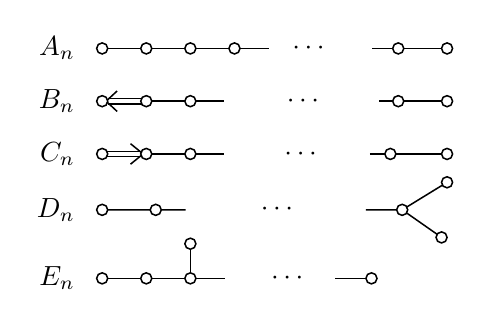
\begin{tikzpicture}[line width=.55pt,vertex/.style={circle,draw,fill=white,inner sep=0pt,minimum size=4pt}]
\node[anchor=east] at (-.22,0) {\(A_n\)};
\node[anchor=east] at (-.22,-.67) {\(B_n\)};
\node[anchor=east] at (-.22,-1.34) {\(C_n\)};
\node[anchor=east] at (-.22,-2.05) {\(D_n\)};
\node[anchor=east] at (-.22,-2.92) {\(E_n\)};
\draw (0,0)--(2.12,0) (3.43,0)--(4.38,0);
\draw (.56,-.67)--(1.55,-.67) (3.52,-.67)--(4.38,-.67);
\draw (.56,-1.34)--(1.55,-1.34) (3.40,-1.34)--(4.38,-1.34);
\draw (.08,-.637)--(.56,-.637) (.08,-.703)--(.56,-.703);
\draw (.19,-.54)--(.05,-.67)--(.19,-.80);
\draw (0,-1.307)--(.48,-1.307) (0,-1.373)--(.48,-1.373);
\draw (.36,-1.21)--(.52,-1.34)--(.36,-1.47);
\draw (0,-2.05)--(1.06,-2.05) (3.35,-2.05)--(3.81,-2.05)
  --(4.38,-1.70) (3.81,-2.05)--(4.31,-2.40);
\draw (0,-2.92)--(1.56,-2.92) (2.96,-2.92)--(3.42,-2.92) (1.12,-2.92)--(1.12,-2.48);
\node at (2.62,0) {\(\cdots\)};
\node at (2.55,-.67) {\(\cdots\)};
\node at (2.52,-1.34) {\(\cdots\)};
\node at (2.22,-2.05) {\(\cdots\)};
\node at (2.35,-2.92) {\(\cdots\)};
\foreach \x in {0,.56,1.12,1.68,3.76,4.38} {\node[vertex] at (\x,0) {};}
\foreach \x in {0,.56,1.12,3.76,4.38} {\node[vertex] at (\x,-.67) {};}
\foreach \x in {0,.56,1.12,3.66,4.38} {\node[vertex] at (\x,-1.34) {};}
\foreach \x in {0,.68,3.81} {\node[vertex] at (\x,-2.05) {};}
\node[vertex] at (4.38,-1.70) {};
\node[vertex] at (4.31,-2.40) {};
\foreach \x in {0,.56,1.12,3.42} {\node[vertex] at (\x,-2.92) {};}
\node[vertex] at (1.12,-2.48) {};
\end{tikzpicture}}\endgroup\par
Левый столбец схем \(A_n,B_n,C_n,D_n,E_n\).}
\end{GelfandAdjacentEvidence}
\begin{GelfandAdjacentEvidence}{GELFAND-P000648}{7}


\SourceFigure{GELFAND-P000648}{dynkin-right}{%
\par\smallskip
\begingroup\color{black}\GelfandFitDiagram{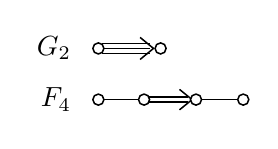
\begin{tikzpicture}[line width=.55pt,vertex/.style={circle,draw,fill=white,inner sep=0pt,minimum size=4pt}]
\node[anchor=east] at (-.22,0) {\(G_2\)};
\node[anchor=east] at (-.22,-.65) {\(F_4\)};
\foreach \y in {-.064,0,.064} {\draw (.04,\y)--(.65,\y);}
\draw (.53,.14)--(.70,0)--(.53,-.14);
\draw (0,-.65)--(.58,-.65) (1.24,-.65)--(1.84,-.65);
\draw (.58,-.617)--(1.14,-.617) (.58,-.683)--(1.14,-.683);
\draw (1.03,-.52)--(1.19,-.65)--(1.03,-.78);
\foreach \x in {0,.79} {\node[vertex] at (\x,0) {};}
\foreach \x in {0,.58,1.24,1.84} {\node[vertex] at (\x,-.65) {};}
\end{tikzpicture}}\endgroup\par
Правый столбец схем \(G_2,F_4\).}
\end{GelfandAdjacentEvidence}
\begin{GelfandAdjacentEvidence}{GELFAND-P000648}{8}


[Справа] и ещё при \(n=6,7,8\).

\begin{center}\(\longrightarrow\)\end{center}
[Слева] \underline{Ройтер.}

Сх. Дынкина --- целочисл. квадр. форма
\[
\sum a_i x_i^2+\sum_{i<j}b_{ij}x_i x_j.
\]
доп. условия 1) положит. определённость.
\quad 2) \(a_i>0\).
\quad 3) \(b_{ij}\leqslant0\).
\quad 4) \(a_i\mid b_{ij}\) (делит).

[Справа] \(\Vert\) получ. в точности сх. Дынкина.

\SourceFigure{GELFAND-P000648}{valued-edge}{%
\par\smallskip
\begingroup\color{black}\GelfandFitDiagram{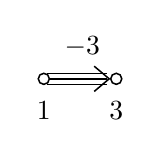
\begin{tikzpicture}[line width=.55pt,vertex/.style={circle,draw,fill=white,inner sep=0pt,minimum size=4pt}]
\foreach \y in {-.07,0,.07} {\draw (.04,\y)--(.80,\y);}
\draw (.64,.16)--(.83,0)--(.64,-.16);
\node[vertex] at (0,0) {};
\node[vertex] at (.92,0) {};
\node[below] at (0,-.16) {\(1\)};
\node[below] at (.92,-.16) {\(3\)};
\node[above] at (.49,.15) {\(-3\)};
\end{tikzpicture}}\endgroup\par
Нижняя схема с числами \(1\) и \(3\) под кружками. Штрих над стрелкой перед \(3\) похож на минус.}
\end{GelfandAdjacentEvidence}


\(\Vert\) \underline{Расшир. схема} --- если замен. усл. на неотриц. определённость.


\Needspace{7\baselineskip}
\begin{GelfandAdjacentEvidence}{GELFAND-P000649}{1}
\SourcePage{GELFAND-P000649}{unlabelled}
Отражение --- замена одной из коорд. вектора, не меняющая кв. формы. (лин. преобр.).

Породим группу всеми отраж.

Простой корень --- \((0,0,\ldots,1,\ldots,0)\).

\underline{Корень:} вектор, получ. из простого неск. отражениями.

Есть вектор \((x_1,\ldots,x_n)\). Когда он корень?

Если все чёрт. однократные, то корень \(\Longleftrightarrow\) кв. форма на нём равна 1.
\Unclear{GELFAND-P000649}{single-strokes}{Сокращение перед «однократные» читается «чёрт.».}
\end{GelfandAdjacentEvidence}
\begin{GelfandAdjacentEvidence}{GELFAND-P000649}{2}


[Зачёркнуто: Если не все однокр.] Если не все однокр.?
\Unclear{GELFAND-P000649}{cancel-not-all}{Первое «Если не все однокр.» перечёркнуто несколькими штрихами.}
\end{GelfandAdjacentEvidence}
\begin{GelfandAdjacentEvidence}{GELFAND-P000649}{3}


\underline{Теор.}
\[
(x_1,\ldots,x_n)\text{ --- корень}\quad\Longleftrightarrow\quad
\forall i:\ f(x)\mid a_i x_i.
\]

\underline{Задача} (для первокурсников).
\[
\sum_{i=1}^{n} a_i x_i^2-\sum_{i<j}b_{ij}x_ix_j,
\qquad \frac{b_{ij}}{a_i}\in\mathbb{Z},\quad a_i>0.
\]

\SourceFigure{GELFAND-P000649}{star-drawing}{%
\par\smallskip
\begingroup\color{black}\GelfandFitDiagram{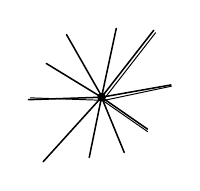
\begin{tikzpicture}[line cap=round,scale=.78]
\draw[line width=.55pt] (0,0)--(-1.19,-.04)
  (0,0)--(-.90,.55) (0,.02)--(-.57,1.02)
  (0,0)--(.24,1.12) (0,0)--(.85,1.09)
  (0,0)--(1.13,.20) (0,0)--(.75,-.52)
  (0,0)--(.37,-.90) (0,0)--(-.20,-.98) (0,0)--(-.95,-1.05);
\draw[line width=.35pt] (.04,-.03)--(.88,1.05)
  (.05,-.05)--(1.14,.18) (.03,-.06)--(.75,-.56)
  (.01,-.05)--(-1.16,-.01);
\fill (0,0) circle[radius=2pt];
\end{tikzpicture}}\endgroup\par
Лучи слева от следующей формулы. Некоторые штрихи сдвоены.}
\end{GelfandAdjacentEvidence}
\begin{GelfandAdjacentEvidence}{GELFAND-P000649}{4}

\[
x_0^2+\cdots+x_n^2-x_0x_1-x_0x_2-\cdots-x_0x_n.
\quad \text{неясно.}
\]

Отраж. --- лин. преобр., не меняющее \(f(x)\) и замен. лишь одну коорд.

[Зачёркнуто: \(x\to\bar x\) и пр\ldots в., подобное.]
\Incomplete{GELFAND-P000649}{cancel-description}{Внутренние буквы перечёркнутого сокращения различимы лишь частично.}
\end{GelfandAdjacentEvidence}

опис. все корни! (получ. отраж. из станд. векторов) (\underline{ВОЛК}\(\to\)КОЗА).

[Справа, столбец]
\begin{gather*}
\text{ВОЛК}\\
\text{ПОЛК}\\
\text{ПОЛА}\\
\text{ПОЗА}\\
\text{КОЗА}
\end{gather*}

\begin{center}\textemdash\enspace\textperiodcentered\enspace\textemdash\end{center}

\underline{Кириллов по поводу докл. Березина.}
\[
x_i x_k=x_k x_i,\qquad x_1,\ldots,x_p
\]
\[
\xi_i\xi_k=-\xi_k\xi_i,\qquad \xi_1,\ldots,\xi_q
\]
\underline{Супермногообразие:} Березин, Лейтес.

[На левом поле] \underline{По Рудакову.}

Рассм. многообразие \(M^p\) и расслоение \(E\to M^p\), слой к-рого ---
\underline{грассманова алгебра} (с \(q\) образующими)
(структ. --- своя в \(\forall\) точке).

Морфизмы описываются сложнее.

Ф-я на супермн. --- гладкое сеч. расслоения.

Правила интегрирования. по \(x\) как обычно и
\[
\int d\xi=0,\qquad \int\xi\,d\xi=1.
\]

Предст. 64-мерной супералгебры Ли лучше описывают элем. част., чем предст. \(SU(3)\).

Замена пер.:
\[
\begin{cases}
x\to x+\xi_1\xi_2,\\
\xi_1\to\xi_1+x\xi_2,\\
\xi_2\to\xi_2+\xi_1\xi_2\xi_3
\end{cases}
\]
\[
\int P(\xi_1,\xi_2,\xi_3)\,d\xi_1\,d\xi_2\,d\xi_3
=\text{коэфф. при старшем члене.}
\]

\underline{Супералгебра Ли:} \(\mathbb Z_2\)-град. и
\[
[x,y]=-(-1)^{\deg x\cdot\deg y}[y,x].
\]

Тожд. Якоби \([x,\cdot]\) --- однородное дифференцирование.

\underline{более уд. опр.:} супералг. получ. из град. ассоц. алгебры по правилу
\[
[x;y]=xy-(-1)^{\deg x\cdot\deg y}yx.
\]

Теор. Ли --- Березин и киевский Кац.

\begin{GelfandAdjacentEvidence}{GELFAND-P000649}{5}
\underline{Замечание Г.} \(p(t+\xi)=p(t)+p'(t)\xi\). Малые только 1\textsuperscript{го} порядка.
\Unclear{GELFAND-P000649}{first-order-phrase}{Первое слово читается предположительно «Малые».}
\end{GelfandAdjacentEvidence}



\Needspace{7\baselineskip}
\begin{GelfandAdjacentEvidence}{GELFAND-P000650}{1}
\SourcePage{GELFAND-P000650}{unlabelled}
Ф-и на супермн. --- супералгебра.

Есть скобка Пуассона.

Найти деформации в напр. скобки Пуассона.

\underline{Синай.}\quad Теор. фаз. перех. --- спектр матриц.

Удалось выч. из инт. примеров один.
\Unclear{GELFAND-P000650}{sinai-examples}{Сокращение после «из» читается предположительно «инт.».}
\end{GelfandAdjacentEvidence}
\begin{GelfandAdjacentEvidence}{GELFAND-P000650}{2}


Размерность пр-ва \(2^n\).
\[
\begin{gathered}
a_{ij}\qquad a(\underbrace{x_1,\ldots,x_n}_{i},\underbrace{y_1,\ldots,y_n}_{j})\\
={e}^{\beta\left(J_1\sum_{i=1}^n x_i x_{i-1}
                  +J_2\sum_{i=1}^n x_i y_i\right)}.
\end{gathered}
\]
\(x_k=\pm1\), \underline{\(x_0=x_n\)}.
\Unclear{GELFAND-P000650}{spin-index}{Индекс при \(x\) густо переписан и похож на \(k\).}
\end{GelfandAdjacentEvidence}
\begin{GelfandAdjacentEvidence}{GELFAND-P000650}{3}


\underline{Физич. задача:} надо изуч. \(\dfrac{e^{-\beta H}}{Z}\). Здесь [зачёркнуто]
\Incomplete{GELFAND-P000650}{cancel-here}{Короткий фрагмент после «Здесь» густо зачёркнут.}
\end{GelfandAdjacentEvidence}
\begin{GelfandAdjacentEvidence}{GELFAND-P000650}{4}

\[
\underline{\frac{\ln Z}{R^2}\underset{R\to\infty}{\longrightarrow}f(\beta).}
\]
Ф-и \(f(\beta)\) могут иметь особ.

Изуч. \(f(\beta)\) --- [зачёркнуто]
\Incomplete{GELFAND-P000650}{cancel-study}{Короткое слово перед «имеется» густо зачёркнуто.}
\end{GelfandAdjacentEvidence}
\begin{GelfandAdjacentEvidence}{GELFAND-P000650}{5}

имеется трансферматрица (transfer-matrix).

Матр. с полож. элем.
\SourceFigure{GELFAND-P000650}{lattice-diagram}{%
\par\smallskip
\begingroup\color{black}\GelfandFitDiagram{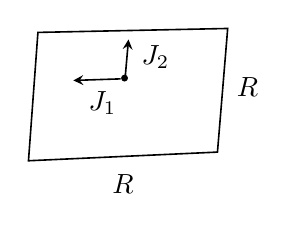
\begin{tikzpicture}[line width=.58pt,>=stealth]
\draw (0,0)--(2.40,.11)--(2.53,1.68)--(.12,1.63)--cycle;
\fill (1.22,1.05) circle[radius=1.25pt];
\draw[->] (1.17,1.04)--(.57,1.02);
\draw[->] (1.23,1.08)--(1.27,1.54);
\node[below] at (.94,1.01) {\(J_1\)};
\node[right] at (1.31,1.32) {\(J_2\)};
\node[right] at (2.52,.94) {\(R\)};
\node[below] at (1.20,-.05) {\(R\)};
\end{tikzpicture}}\endgroup\par
Стрелки направлены влево и вверх. Подписи читаются как \(J_1\) и \(J_2\).}
\end{GelfandAdjacentEvidence}
\begin{GelfandAdjacentEvidence}{GELFAND-P000650}{6}

\[
Z=\sum e^{-\beta\sum_{x',x''}H(x',x'')},
\qquad \underline{Z=\operatorname{tr}A^R}.
\]
\Unclear{GELFAND-P000650}{trace-exponent}{Верхний индекс густо переписан и читается как \(R\).}
\end{GelfandAdjacentEvidence}

\(A^R\) --- матр. перех. от слоя к слою.

\underline{(2-мерная зад. Онзагера).}

\underline{Онзагер выч. все соб. значения этой матрицы:}

Здесь помогают антикомм. переменные: есть такие антикомм. матр. \(A_i,A_j\), такие что
\[
A=e^{\sum c_{ij}A_i A_j}
\]
и интегралы считаются.

[На правом поле] \(\Vert\) см. \underline{Хуанг} «\underline{Стат. мех.}».

\underline{Либ} аналог. считал энтропию квадр. льда.

\begin{center}\textemdash\enspace\textperiodcentered\enspace\textemdash\end{center}


\Needspace{7\baselineskip}
\begin{GelfandAdjacentEvidence}{GELFAND-P000651}{1}
\SourcePage{GELFAND-P000651}{unlabelled}
\underline{29/III-76.}\quad \underline{Сем. Гельфанда.}

\underline{Кричевер:}\quad \underline{задача:} решить ур-е \([L_1,L_2]=0\).
Если \(\operatorname{ord}L_1\) и \(\operatorname{ord}L_2\) вз. пр., то ответ --- кривая и расслоение
(1-мерное).

Порядки не вз. просты --- возникают многомерные пучки.

Напр., \underline{4-й и 6-й пор. --- не сделано}. Свед. к 2-мерным расслоениям.
\[
\left.\begin{aligned}
L_1y&=E_1y\\
L_2y&=E_2y
\end{aligned}\right\}
\quad P(E_1,E_2)=0\quad\text{--- кривая.}
\]
\Incomplete{GELFAND-P000651}{cancel-bundle}{Под скобкой совместных уравнений густо замаранный фрагмент.}
\end{GelfandAdjacentEvidence}
\begin{GelfandAdjacentEvidence}{GELFAND-P000651}{2}

Совм. решение --- 2-мерн. рассл. над кривой.

Вз. просты --- базис 1-мерный. (из асимптотики).

\((m,n)=1\Longrightarrow\) общ. соб. ф-й равно \(n\). (и соб. знач. различны)

\(E_1\) опр. по \(E\); \(y\) однозн. опр. ф-я на рим. пов.
\Unclear{GELFAND-P000651}{eigenvalue-overwrite}{Индекс первого \(E\) читается предположительно как \(1\). Слово «по» густо переписано.}
\end{GelfandAdjacentEvidence}
\begin{GelfandAdjacentEvidence}{GELFAND-P000651}{3}


\underline{Обр. зад.:} по расслоению построить коммут. дифф. оп. --- не сделано.

\underline{Дринфельд.}
\[
d=(m,n)\Longrightarrow\quad
\text{зад. пары комм. оп.}\quad\Longleftrightarrow\quad
\text{зад. \((d-1)\) произв. ф-и}
\]

\(B^{-1}LB\) разрешим. --- ост. 1 произв. ф-я --- старший коэфф.

4 и 6 пор. --- если квадр. и кубик --- уже 2 произв. ф-и.

\underline{\underline{Шнирельман.}}\quad \(M\) --- \(n\)-мерное риманово комп. аналит. мн-ие,

\(\Delta\) --- оп. Лапласа на \(M\);
\[
\underline{\Delta u_k+\lambda_k^2u_k=0;}\qquad(1)
\]

\underline{опред. \(\Delta\):}
\SourceFigure{GELFAND-P000651}{sphere-sketch}{%
\par\smallskip
\begingroup\color{black}\GelfandFitDiagram{\begin{tikzpicture}[line width=.55pt]
\draw (0,0) ellipse[x radius=.34,y radius=.29];
\fill (-.025,-.005) circle[radius=1.1pt];
\node[right] at (.50,0) {сф. рад. \(\tau\);};
\end{tikzpicture}}\endgroup\par
Кружок с точкой в центре.}
\end{GelfandAdjacentEvidence}
\begin{GelfandAdjacentEvidence}{GELFAND-P000651}{4}

\[
\frac{\text{ср. по сфере рад. \(\tau\) --- зн. в центре}}{\tau^2}
\longrightarrow\Delta f(x).
\]

\underline{Рост с ростом \(k\):}\quad \(\lambda_k\sim c k^{1/n}\), [зачёркнуто: \(a\ldots\)]
\Incomplete{GELFAND-P000651}{cancel-square}{Под перечёркиванием в начале виден знак, похожий на \(a\).}
\end{GelfandAdjacentEvidence}
\begin{GelfandAdjacentEvidence}{GELFAND-P000651}{5}


Пусть \(a>0\). Как распр. \(\underline{a\cdot\lambda_k\bmod 2\pi}\)

(Часто есть арифм. прогрессии).

\qquad --- подпослед.

\underline{Тор.}
\SourceFigure{GELFAND-P000651}{torus-rectangle}{%
\par\smallskip
\begingroup\color{black}\GelfandFitDiagram{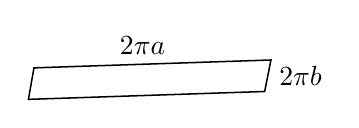
\begin{tikzpicture}[line width=.55pt]
\draw (0,0)--(3.0,.10)--(3.08,.50)--(.07,.40)--cycle;
\node[above] at (1.45,.44) {\(2\pi a\)};
\node[right] at (3.06,.30) {\(2\pi b\)};
\end{tikzpicture}}\endgroup\par
Прямоугольник под надписью «Тор».}
\end{GelfandAdjacentEvidence}
\begin{GelfandAdjacentEvidence}{GELFAND-P000651}{6}

\[
\Delta u=\lambda^2u.
\]
\(\sin\alpha x\cdot\sin\beta y\)
[зачёркнуто: \(\cos\ldots\)]
\Incomplete{GELFAND-P000651}{cancel-sine}{Начало зачёркнутой записи похоже на \(\cos\). Остальные знаки неразборчивы.}
\end{GelfandAdjacentEvidence}
\begin{GelfandAdjacentEvidence}{GELFAND-P000651}{7}

или \(\cos\alpha x\cdot\sin\beta y\) и т. д.
\[
\lambda^2=\frac{n^2}{a^2}+\frac{m^2}{b^2},\qquad
\lambda=\sqrt{\frac{n^2}{a^2}+\frac{m^2}{b^2}}.
\]
Серии --- при разных \(n\) и \(m\) (при фиксир.).

Какие 2 номера --- неясно.

\underline{Теор. об 1-м мер.}
\Unclear{GELFAND-P000651}{first-dimension}{Последнее сокращение предположительно читается «мер.».}
\end{GelfandAdjacentEvidence}
\begin{GelfandAdjacentEvidence}{GELFAND-P000651}{8}

\[
-y''+u(x)y=\lambda y\quad\Longrightarrow\quad\text{на}
\]
\SourceFigure{GELFAND-P000651}{interval-sketch}{%
\par\smallskip
\begingroup\color{black}\GelfandFitDiagram{\begin{tikzpicture}[line width=.55pt]
\draw (0,0)--(1.45,0) (0,-.09)--(0,.09) (1.45,-.09)--(1.45,.09);
\end{tikzpicture}}\endgroup\par
Горизонтальная черта с двумя концевыми черточками.}
\end{GelfandAdjacentEvidence}
\begin{GelfandAdjacentEvidence}{GELFAND-P000651}{9}

\[
\sum_{i=0}^{n-1}c_i y_i\quad\text{имеет \(\leq n\) нулей}
\quad\Longrightarrow\quad\text{ведёт себя как мног. 1-й степ.}
\]

Отсюда 2 мер. --- многочлен от \(n\) перем.
\Unclear{GELFAND-P000651}{second-dimension}{Сокращение после цифры 2 предположительно читается «мер.».}
\end{GelfandAdjacentEvidence}
\begin{GelfandAdjacentEvidence}{GELFAND-P000651}{10}


\underline{Наименьш. --- всюду положит.}

\underline{1-я} --- как лин. ф-и.

Далее --- кривая 2-го пор.

следить за лин. комбин.
\SourceFigure{GELFAND-P000651}{oval-chords}{%
\par\smallskip
\begingroup\color{black}\GelfandFitDiagram{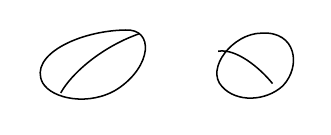
\begin{tikzpicture}[line width=.55pt]
\draw (-.85,0) .. controls (-1.03,.35) and (-.39,.66) .. (.20,.67)
 .. controls (.57,.69) and (.54,.21) .. (.10,-.08)
 .. controls (-.25,-.30) and (-.73,-.21) .. (-.85,0);
\draw (-.62,-.13) .. controls (-.49,.11) and (-.11,.45) .. (.37,.62);
\draw (1.43,-.05) .. controls (1.21,.18) and (1.57,.63) .. (1.93,.63)
 .. controls (2.37,.66) and (2.44,.21) .. (2.20,-.04)
 .. controls (1.98,-.24) and (1.61,-.25) .. (1.43,-.05);
\draw (1.38,.40) .. controls (1.60,.44) and (1.90,.20) .. (2.07,-.01);
\end{tikzpicture}}\endgroup\par
Два овала. В левом наклонная линия идёт от внутренней точки к верхнему краю, в правом --- от левого края к внутренней точке.}
\end{GelfandAdjacentEvidence}


\underline{\underline{Рэлей}} --- теория звука (2 тома).

\underline{Арнольд:} перенести теор. Харнака о числе овалов (у лин. комб. неизвестно).

[На правом поле] \(\Vert\) У \(n\)-й соб. ф-и нули делят обл. \(\leq\) на \(n\) частей.


\Needspace{7\baselineskip}
\begin{GelfandAdjacentEvidence}{GELFAND-P000652}{1}
\SourcePage{GELFAND-P000652}{unlabelled}
Рассмотрим
\[
\Phi(\lambda,a)=\lim_{\varepsilon\to0}\varepsilon
\left(\sum\delta((\lambda-a\lambda_k)\bmod 2\pi)e^{-\varepsilon\lambda_k}
-\sum_k\frac{e^{-\varepsilon\lambda_k}}{2\pi}\right).
\]
\[
\mu_k=a\lambda_k\bmod 2\pi.
\]
\(\mu\) --- пар. на окр.
\Unclear{GELFAND-P000652}{distribution-letter}{Густо обведённая буква читается предположительно \(\mu\). Дальше «пар. на окр.».}
\end{GelfandAdjacentEvidence}
\begin{GelfandAdjacentEvidence}{GELFAND-P000652}{2}

\[
\Phi(\mu,a)=\lim_{\varepsilon\to0}\varepsilon
\left(\sum_{k=1}^{\infty}\delta(\mu-\mu_k)e^{-\varepsilon\lambda_k}
-\sum e^{-\varepsilon\lambda_k}/2\pi\right).
\]
[Стрелка к вычитаемому члену] вычесть, чтобы ср. знач. было \(0\). постоянная.

\(\Phi^\varepsilon(\mu,a)\) --- допред. выражение.

\underline{Теорема.} Пусть \(\gamma_1,\gamma_2,\ldots\) --- замкнутые геодезич. на \(M\),
\(\ell(\gamma_1),\ell(\gamma_2),\ldots\) --- их длины.
Пусть невд. расп.,
\Unclear{GELFAND-P000652}{nondegenerate-abbreviation}{Первое сокращение похоже на «невд.». За ним читается «расп.».}
\end{GelfandAdjacentEvidence}
\begin{GelfandAdjacentEvidence}{GELFAND-P000652}{3}

дискр. обр.,
\Unclear{GELFAND-P000652}{dispersion-abbreviation}{Первое сокращение предположительно читается «дискр.».}
\end{GelfandAdjacentEvidence}
\begin{GelfandAdjacentEvidence}{GELFAND-P000652}{4}

длины все разл. и несоизмеримы. (общее полож.).
\[
\Phi(\mu,a)\left\{
\begin{aligned}
&\equiv0&&\text{если } a\ne\frac pq\ell(\gamma_j),\\
&\not\equiv0&&\text{[зачёркнуто] если } a=\frac pq\ell(\gamma_j).
\end{aligned}
\right.
\quad(p,q\in\mathbb Z)
\]
\Incomplete{GELFAND-P000652}{cancel-if}{Слово перед вторым «если» густо перечёркнуто.}
\end{GelfandAdjacentEvidence}
\begin{GelfandAdjacentEvidence}{GELFAND-P000652}{5}


[На левом поле]
\SourceFigure{GELFAND-P000652}{geodesic-loop}{%
\par\smallskip
\begingroup\color{black}\GelfandFitDiagram{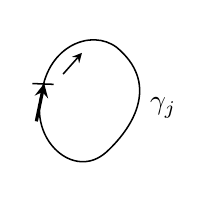
\begin{tikzpicture}[line width=.55pt,>=stealth]
\draw (-.57,.06) .. controls (-.49,.66) and (.06,.88) .. (.38,.64)
 .. controls (.91,.20) and (.63,-.34) .. (.25,-.69)
 .. controls (-.16,-1.06) and (-.74,-.53) .. (-.57,.06);
\draw[line width=1.15pt,->] (-.64,-.30)--(-.54,.18);
\draw (-.69,.18)--(-.42,.17);
\draw[->] (-.30,.30)--(-.06,.57);
\node[right] at (.68,-.13) {\(\gamma_j\)};
\end{tikzpicture}}\endgroup\par
Овал и стрелки. На левом крае толстые штрихи накладываются друг на друга.}
\end{GelfandAdjacentEvidence}
\begin{GelfandAdjacentEvidence}{GELFAND-P000652}{6}

рассм. геодезич. поток. (\(\in SM\)).

\(S\) --- площ., трансверс. замкн. геод. (разм. \(2n-2\)).

отобр. последования \(\Psi:S\to S\).

\(S\cap\gamma_j\) --- неподв. точка.
\[
d\Psi\big|_{S\cap\gamma_j}=\mathcal M
\quad\text{--- опер. монодромии}\quad\text{(\underline{матр. монодромии})}.
\]
Это преобр. \underline{симплектично}, т. к. поток гамильтонов.

Соб. числа расп. на пары и четвёрки.
\SourceFigure{GELFAND-P000652}{eigenvalue-drawings}{%
\par\smallskip
\begingroup\color{black}\GelfandFitDiagram{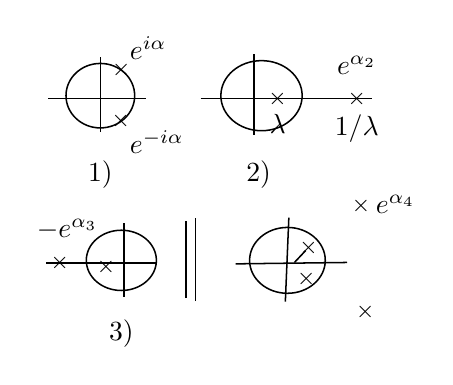
\begin{tikzpicture}[line width=.55pt,scale=.89,
cross/.style={inner sep=0pt,font=\footnotesize}]
\begin{scope}[xshift=.1cm]
\draw (0,0) ellipse[x radius=.49,y radius=.46];
\draw (-.74,-.04)--(.65,-.04) (0,-.52)--(0,.55);
\node[cross] at (.30,.37) {\(\times\)};
\node[cross] at (.29,-.36) {\(\times\)};
\node[above right] at (.28,.37) {\(e^{i\alpha}\)};
\node[below right] at (.28,-.36) {\(e^{-i\alpha}\)};
\node[below] at (0,-.78) {1)};
\end{scope}
\begin{scope}[xshift=2.33cm]
\draw (.07,0) ellipse[x radius=.58,y radius=.50];
\draw (-.80,-.04)--(1.64,-.04) (-.04,-.56)--(-.04,.59);
\node[cross] at (.30,-.04) {\(\times\)};
\node[cross] at (1.43,-.04) {\(\times\)};
\node[below] at (.30,-.13) {\(\lambda\)};
\node[above] at (1.43,.16) {\(e^{\alpha_2}\)};
\node[below] at (1.43,-.13) {\(1/\lambda\)};
\node[below] at (.03,-.78) {2)};
\end{scope}
\begin{scope}[yshift=-2.35cm,xshift=.40cm]
\draw (0,0) ellipse[x radius=.50,y radius=.43];
\draw (-1.07,-.04)--(.49,-.04) (.04,-.52)--(.04,.54);
\node[cross] at (-.88,-.04) {\(\times\)};
\node[cross] at (-.22,-.09) {\(\times\)};
\node[above] at (-.77,.15) {\(-e^{\alpha_3}\)};
\node[below] at (0,-.71) {3)};
\draw (.92,-.54)--(.92,.56) (1.06,-.58)--(1.06,.60);
\end{scope}
\begin{scope}[xshift=2.77cm,yshift=-2.35cm]
\draw (0,0) ellipse[x radius=.54,y radius=.47];
\draw (-.74,-.05)--(.85,-.03) (-.03,-.59)--(.02,.61);
\draw (.10,-.03)--(.26,.14);
\node[cross] at (.30,.18) {\(\times\)};
\node[cross] at (.27,-.26) {\(\times\)};
\node[cross] at (1.05,.77) {\(\times\)};
\node[cross] at (1.11,-.73) {\(\times\)};
\node[right] at (1.12,.80) {\(e^{\alpha_4}\)};
\end{scope}
\end{tikzpicture}}\endgroup\par
Три нумерованные схемы и четвёртая без номера. У внутреннего креста в третьей схеме уверенно читаемой подписи нет.}
\end{GelfandAdjacentEvidence}
\begin{GelfandAdjacentEvidence}{GELFAND-P000652}{7}


[Справа от четвёртой схемы] --- это только в 3-мерн. пр-ве.

\underline{Рассм. коэфф. Фурье:}
\[
\varphi_n(a)=\int_0^{2\pi}\varphi(\mu,a)e^{-i\mu n}\,d\mu.
\]
\begin{align*}
1)\quad\varphi_n(a)&=\frac{c}{\sin\dfrac{n\alpha_1}{2}},\\
2)\quad\varphi_n(a)&=\frac{c}{\operatorname{sh}\dfrac{n\alpha_2}{2}},\\
3)\quad\varphi_n(a)&=(-1)^n\frac{c}{\operatorname{sh}\dfrac{n\alpha}{2}}.
\end{align*}
\(c\) зависит от размерности.

[Длинная охватывающая линия от трёх формул к записи справа.]

\(1)\quad\alpha_1\) плохо прибл. рацион. (треб.) \(\Longrightarrow\)
\Unclear{GELFAND-P000652}{approximation-verb}{Перед «прибл.» написано «плохо».}

\Unclear{GELFAND-P000652}{approximation-parenthesis}{В скобках предположительно «треб.».}
\end{GelfandAdjacentEvidence}
\begin{GelfandAdjacentEvidence}{GELFAND-P000652}{9}

\[
\text{A)}\quad
\varphi(\mu,a)=\sum_{n=0}^{\infty}
\delta\left(\mu-\left(n+\frac12\right)\alpha-\frac1{2\pi}\right).
\]

(точно в рег. смысле
\[
\varphi(\mu,a)=\lim_{\varepsilon\to0}\sum_{n=0}^{\infty}
\delta\left(\mu-\left(n+\frac12\right)\alpha e^{-n\varepsilon}-\frac1{2\pi}\right).
\]

[На нижнем левом поле] \underline{2 квант. числа} --- 2 индекса.

[На нижнем левом поле] [густой знак] Беск. число ар. прогрессий.
\Incomplete{GELFAND-P000652}{progression-mark}{Перед строкой густой знак, похожий на букву А.}
\end{GelfandAdjacentEvidence}



\Needspace{7\baselineskip}
\begin{GelfandAdjacentEvidence}{GELFAND-P000653}{1}
\SourcePage{GELFAND-P000653}{unlabelled}
\[
\begin{aligned}
2)\quad\varphi(\mu,a)
&=c\sum_{m,n=-\infty}^{\infty}
\left(
\frac1{\mu-n\cdot2\pi-(m+\frac12)i}
+\frac1{n\cdot2\pi+(m+\frac12)i\,\text{[зач. знак]}}
\right)\\
&=c\int_0^\mu\wp(\xi)\,d\xi,
\end{aligned}
\]
\(\wp\) --- ф-я Вейерштрасса.
\Unclear{GELFAND-P000653}{period-end}{После \(i\) во втором знаменателе штрих с несколькими поперечными чертами. Зачёркнутая буква не установлена.}
\end{GelfandAdjacentEvidence}
\begin{GelfandAdjacentEvidence}{GELFAND-P000653}{2}


\SourceFigure{GELFAND-P000653}{pole-lattice}{%
\par\smallskip
\begingroup\color{black}\GelfandFitDiagram{\begin{tikzpicture}[line width=.58pt,>=stealth]
\draw (-1.24,-.08)--(1.13,.03) (0,-.78)--(0,.88);
\foreach \x/\y in {0/.51,1.24/.56,0/-.68,1.15/-.70}
 {\node[inner sep=0pt] at (\x,\y) {\(\times\)};}
\draw[->] (2.12,-.19)--(1.65,-.20);
\node[right] at (2.14,-.19) {полюса};
\end{tikzpicture}}\endgroup\par
Кресты на вертикальной оси и справа от неё.}
\end{GelfandAdjacentEvidence}
\begin{GelfandAdjacentEvidence}{GELFAND-P000653}{3}


\SourceFigure{GELFAND-P000653}{curve-figure}{%
\par\smallskip
\begingroup\color{black}\GelfandFitDiagram{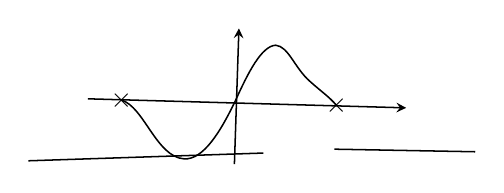
\begin{tikzpicture}[line width=.55pt,>=stealth,x=.82cm,y=.82cm]
\draw[->] (-2.30,.04)--(2.63,-.10);
\draw[->] (-.03,-.97)--(.04,1.13);
\draw (-3.22,-.92)--(.42,-.80) (1.52,-.74)--(3.70,-.78);
\draw (-1.78,.02) .. controls (-1.43,-.08) and (-1.24,-.86) .. (-.81,-.89)
 .. controls (-.51,-.91) and (-.24,-.46) .. (-.01,.02)
 .. controls (.18,.44) and (.39,.86) .. (.61,.87)
 .. controls (.81,.85) and (.90,.52) .. (1.14,.31)
 .. controls (1.33,.14) and (1.44,.07) .. (1.55,-.06);
\node[inner sep=0pt] at (-1.78,.02) {\(\times\)};
\node[inner sep=0pt] at (1.55,-.06) {\(\times\)};
\end{tikzpicture}}\endgroup\par
Кривая с минимумом и максимумом, два креста на оси и нижняя прерывистая черта. Под левым отрезком черты густой неразборчивый знак.}
\end{GelfandAdjacentEvidence}
\begin{GelfandAdjacentEvidence}{GELFAND-P000653}{4}


Рассм. ф-я
\[
f(z)=\sum_{k=1}^{\infty}e^{i\lambda_k z}.
\]
Аналит. продолжается вниз с пр. полюсами.

[Справа]
\SourceFigure{GELFAND-P000653}{hatched-poles}{%
\par\smallskip
\begingroup\color{black}\GelfandFitDiagram{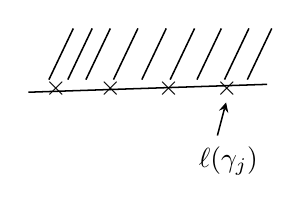
\begin{tikzpicture}[line width=.55pt,>=stealth]
\draw (0,-.02)--(3.03,.08);
\foreach \x in {.26,.50,.73,1.08,1.44,1.80,2.14,2.49,2.78}
 {\draw (\x,.14)--++(.31,.65);}
\foreach \x in {.35,1.04,1.78,2.52}
 {\node[inner sep=0pt] at (\x,.03) {\(\times\)};}
\draw[->] (2.40,-.57)--(2.51,-.15);
\node[below] at (2.54,-.58) {\(\ell(\gamma_j)\)};
\end{tikzpicture}}\endgroup\par
Четыре креста на заштрихованной горизонтали. Стрелка снизу указывает на правый крест.}
\end{GelfandAdjacentEvidence}
\begin{GelfandAdjacentEvidence}{GELFAND-P000653}{5}


Фунд. реш. волн. ур-я. Продолже.

Вычеты в \(\ell(\gamma_j),\,2\ell(\gamma_j),\,\ldots\) --- коэфф. Фурье, и т. д.
\Unclear{GELFAND-P000653}{pole-order}{Буква с индексом \(j\) в подписи и строке вычетов читается как \(\gamma\), как в обозначении геодезической на предыдущем кадре.}
\end{GelfandAdjacentEvidence}
\begin{GelfandAdjacentEvidence}{GELFAND-P000653}{6}

\Unclear{GELFAND-P000653}{fourier-overwrite}{Перед «Фурье» густо наведённое сокращение «коэфф.».}
\end{GelfandAdjacentEvidence}



\Needspace{7\baselineskip}
\begin{GelfandAdjacentEvidence}{GELFAND-P000654}{1}
\SourcePage{GELFAND-P000654}{unlabelled}
5/IV-76.\quad \underline{Сем. Гельфанда.}\quad \underline{Поляков.}

Действие
\[
\left\{\begin{aligned}
S&=\frac1{4e^2}\operatorname{tr}\int A_{\mu\nu}^{2}\,d^4x\\
F_{\mu\nu}&=\partial_\mu A_\nu-\partial_\nu A_\mu+[A_\mu,A_\nu]
\end{aligned}\right.
\]
\Unclear{GELFAND-P000654}{curvature-symbol}{Под интегралом написано \(A_{\mu\nu}^2\). В следующей строке определено \(F_{\mu\nu}\).}
\end{GelfandAdjacentEvidence}
\begin{GelfandAdjacentEvidence}{GELFAND-P000654}{2}

\(A_\mu^+=-A_\mu\),\quad \(A_\mu\) --- косоэрм. матр. \(2\times2\),
явл. ф-ей на \(\mathbb R^4\).

[Под \(A_\mu\)] \(\mu=0,1,2,3\).

\(A_\mu\) --- поле. \(S\) --- ф-л от поля.

Классич. ур-я движ. --- стационарность \(S\).

Для чисел \(A_\mu\) --- эл.-магн. поле.

\underline{Аналог для дискр. \(x\) и \(t\).}
\[
x=(t,\vec{x}).
\]
\SourceFigure{GELFAND-P000654}{lattice-grid}{%
\par\smallskip
\begingroup\color{black}\GelfandFitDiagram{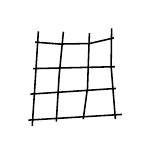
\begin{tikzpicture}[line width=.56pt,scale=.60]
\draw (-.07,0)--(1.91,.12) (-.03,.55)--(1.78,.67)
  (.03,1.09)--(1.76,1.13) (.07,1.65)--(.59,1.61)--(1.22,1.62)--(1.74,1.74);
\draw (.01,-.12)--(.06,.62)--(.14,1.88)
  (.52,-.03)--(.58,.95)--(.67,1.87)
  (1.09,.02)--(1.18,.68)--(1.22,1.84)
  (1.77,.02)--(1.68,1.14)--(1.69,1.94);
\end{tikzpicture}}\endgroup\par
Четыре примерно горизонтальные и четыре вертикальные линии.}
\end{GelfandAdjacentEvidence}
\begin{GelfandAdjacentEvidence}{GELFAND-P000654}{3}

\[
S=\frac{1}{4e_0^2}\sum_{\bar x}\chi\left(
B_{\bar x,\mu} B_{\bar x+\bar a_\mu,\nu}
B^{-1}_{\bar x+\bar a_\nu,\mu} B^{-1}_{\bar x,\nu}
\right).
\]
\Unclear{GELFAND-P000654}{plaquette-notation}{В произведении над \(x\) и \(a\) короткие черты. Черта над первым \(x\) густо наведена.}
\end{GelfandAdjacentEvidence}
\begin{GelfandAdjacentEvidence}{GELFAND-P000654}{4}

\(a_\mu\) --- репер,\qquad \(B_{x,\mu}\in SU(2)\).

\(\chi\) --- любой характер (зачёркнуто)
\Incomplete{GELFAND-P000654}{cancelled-character}{Зачёркнутое слово перед «ф-я» не разобрано.}
\end{GelfandAdjacentEvidence}

(ф-я, пост. на классах сопр. элем. --- например, след).
\[
Z=\int\prod_{\vec x,\mu}dB_{\vec x,\mu}\ e^{-S(B)}.
\]
\(12n\) незав. переменных (\(n\) --- число точек решётки, в \(\forall\) --- 4 матрицы).

\(B_{\vec x,\mu}\) --- незав. пер. \(\Longrightarrow\)
\(dB_{\vec x,\mu}\) --- \underline{инв. мера}
(\(4n\) интегралов по инв. мерам).
\[
t\to it\quad\Longrightarrow\quad e^{iS}\to e^{-S}.
\]
\underline{В непр. случае --- функц. интеграл.}

Коррел. ф-и
\[
\cdots\quad\cdots\quad\cdots\quad\cdots\quad\cdots\quad\cdots
\]


\Needspace{7\baselineskip}
\begin{GelfandAdjacentEvidence}{GELFAND-P000655}{1}
\SourcePage{GELFAND-P000655}{unlabelled}
\underline{12/IV-76.}\quad \underline{Сем. Гельфанда.}

\underline{\underline{Фукс.}}\quad \underline{Применение выч. машин в теор. математике.}

Выч. когом. алгебры форм. бездиверг. вект. полей

Есть \(\mathbb R^n\). Рассмотрим \((\mathbb R^n)'\) и полиномы
\[
p(\xi_1,\ldots,\xi_q;\eta_1,\ldots,\eta_q),\qquad
\xi_i\in\mathbb R^n,\quad\eta_i\in(\mathbb R^n)'.
\]
Они облад. св-вом

а) если пару \(\xi_i,\eta_i\) поставить на место \(\xi_j,\eta_j\), то полином меняет знак.

\(dP=P_1\) зад. ф-лой
\begin{align*}
P_1(\xi_1,\ldots,\xi_{q+1},\eta_1,\ldots,\eta_{q+1})
 &=\sum_{i<j}(-1)^{i+j-1}\big[(\xi_i,\eta_j)-(\xi_j,\eta_i)\big]\\
 &\quad P(\xi_i+\xi_j,\xi_1,\ldots,\widehat\xi_i,\ldots,
                \widehat\xi_j,\ldots,\xi_{q+1},\\
 &\qquad\;\;\eta_i+\eta_j,\eta_1,\ldots,\widehat\eta_i,\ldots,
                 \widehat\eta_j,\ldots,\eta_{q+1}).
\end{align*}

\underline{\underline{задача:}} найти когомологии этого комплекса (до сих пор не сделано).

Выч. машина помогла найти нетрив. циклы.

Рассм. линейные по \(\eta\); тогда это комплекс когом. алгебры \(W_n\).

Не сделано даже для \(n=1\).

Все получ. рез. относятся к этому случаю.

комплекс \(=\) сумме большого числа кон.-мерных.

Суммар. степень по \(\xi\): \(m_1+q\),
\quad по \(\eta\): \(m_2+q\).
\quad [Справа] \(\Vert\) \underline{подкомплекс} \(K_{m_1,m_2}\).

(\(q\) меняется)

\underline{мн-ны от \(\xi_1,\ldots,\xi_q,\eta_1,\ldots,\eta_q\).}
\Unclear{GELFAND-P000655}{polynomial-abbreviation}{Первое сокращение предположительно «мн-ны».}
\end{GelfandAdjacentEvidence}
\begin{GelfandAdjacentEvidence}{GELFAND-P000655}{2}


Каждый из них конечномерен.

\(m_1\ne m_2\Longrightarrow\) он ацикличен.

В действит. \(\sum\) гомол. счётн. числа подкомпл.
\[
H(K)=\bigoplus_m H(K_{m,m}).
\]
(пока \(n\) произвольно)

\underline{\(n=1\)}.

\(m=1,2,3\) ацикличны.

\underline{\(m=4\)} нетрив. в разм. \underline{\(7\) и \(10\)}
--- считали на машине (Гельфанд, Фукс, Калинин).
\Unclear{GELFAND-P000655}{cohomology-name}{Третья фамилия читается «Калинин».}
\end{GelfandAdjacentEvidence}
\begin{GelfandAdjacentEvidence}{GELFAND-P000655}{3}


\underline{\(m=5\)} --- «переполнение рабочего поля \(N=2\)».

\underline{Эйлерова хар-ка} не зав. от дифференциала.

\underline{Першик} (асп. Ботта) досчит. до \underline{\underline{\(m=35\)}}.
\Unclear{GELFAND-P000655}{perchik-name}{В рукописи «Першик».}
\end{GelfandAdjacentEvidence}
\begin{GelfandAdjacentEvidence}{GELFAND-P000655}{4}

\[
K_{m,m}\supset K'_{m,m}\qquad
H(K_{m,m})=H(K'_{m,m})\otimes H(S^3).
\]
\[
\chi_m^*\text{ --- ?}\qquad(\text{для }K'_{m,m}).
\]
\underline{Першик нашёл} производ. ф-ю для \(\chi_m\).
\Unclear{GELFAND-P000655}{series-chi}{После «для» написано \(\chi_m\) без звёздочки.}
\end{GelfandAdjacentEvidence}
\begin{GelfandAdjacentEvidence}{GELFAND-P000655}{5}


Интересно: док., что при сколь угодно больших \(m\) есть \(\chi_m\ne0\).
\Unclear{GELFAND-P000655}{bottom-word-full}{Средние буквы наведены. Слово читается «Интересно».}
\end{GelfandAdjacentEvidence}

\[
\begin{aligned}
&\tfrac12(1-t^{-1}x^{-1})(1-t^{-1}x)\\
&\qquad (1-x^{-2})\qquad (1-x^2)\\
&(1-tx^{-3})(1-tx^{-1})(1-tx)(1-tx^3)\\
&\ldots
\end{aligned}
\]


\Needspace{7\baselineskip}
\begin{GelfandAdjacentEvidence}{GELFAND-P000656}{1}
\SourcePage{GELFAND-P000656}{unlabelled}
\[
(1-t^\ell x^{-\ell-2})(1-t^2x^{-\ell})\ldots(1-t^\ell x^{\ell+2}).
\]
\Unclear{GELFAND-P000656}{middle-t-power}{Средний показатель при \(t\) густо наведён. Видимая форма похожа на \(2\), крайние показатели читаются как \(\ell\).}
\end{GelfandAdjacentEvidence}
\begin{GelfandAdjacentEvidence}{GELFAND-P000656}{2}


Берём произведение всех. Выбрасываем \underline{всё, что сод. \(x\)}. Тогда получится
\[
\sum\chi_m t^{2m}=t^{-2}+2-t^8-t^{14}-t^{22}+\ldots+10t^{70}+\ldots
\]
Написали разл. до \(t^{70}\).

(Доказано сущ. \(\geqslant57\) нетрив. [вписано сверху: кл.] когомологий.)

\underline{\underline{Бухштабер}}\quad \underline{о раб. Адамса о раб. Бухштабера.}

\(X\) --- топ. пр-во. Рассм. \(X\times X\to X\) для группы.
\(\Longrightarrow\)

[Слева, со стрелкой к «Рассм.»] Если \(X\) --- наст. группа, то,
\[
C(X\times X)\longleftarrow C(X)\quad\text{--- структ. коалгебры.}
\]
Грубо:
\[
M(f(x\cdot y))\longleftarrow f(x)
\]
(мат. ожидание значений).

\begin{center}\textemdash\enspace\textperiodcentered\enspace\textemdash\end{center}

\underline{\underline{С. П. Новиков}}\qquad \underline{Общая теор. относительности.}

\underline{Читать:} Ландау и Лифшиц (вместе с рим. геометрией) --- Теор. поля.

\((t,\vec x)\) --- пр-во событий. \((t,\vec x)\to(x^0,\vec x),\quad x^0=ct\).
\[
\underline{ds^2=g_{ij}\,dx^i\,dx^j},
\qquad
g_{ij}=\begin{pmatrix}
1&&&0\\&-1&&\\&&-1&\\0&&&-1
\end{pmatrix}.
\]
Соб. время --- длина кривой.

\underline{Пусть \(M^4\); зад. \(g_{ij}\)}.\qquad
\(U\) --- сист. коорд. \(x^0,x^1,x^2,x^3\).
\Unclear{GELFAND-P000656}{coordinate-symbol}{Знак перед «сист. коорд.» читается предположительно \(U\). Графически похож на «И».}
\end{GelfandAdjacentEvidence}
\begin{GelfandAdjacentEvidence}{GELFAND-P000656}{3}


\underline{Эйнштейн:} метрика наз. гравит. полем (1913) (+ Гроссман)

\underline{Ур-е Эйнштейна} --- незав. Эйнштейн и Гильберт (1916)
\[
\underbrace{R_{ij}-\frac12Rg_{ij}=\frac{8\pi K}{c^4}T_{ij}}.
\]
\Unclear{GELFAND-P000656}{field-equation-k}{В числителе написана прописная \(K\).}
\end{GelfandAdjacentEvidence}
\begin{GelfandAdjacentEvidence}{GELFAND-P000656}{4}


Здесь \(R_{j\ell}=\sum_i R^i_{ji\ell}\) --- тензор Риччи.

[Справа] \(\Vert\) \((R^i_j)_{k\ell}\) --- 2-форма
(кососимм. по \(k,\ell\)) со знач. в алг. Ли гр. \(O(n)\).

\(T_{ij}\) --- тенз. эн.-имп. материи (внешняя масса).

[Справа] \(T_{ij}\) отвеч. за всё, кроме гравит. поля.
\[
R=\sum_{j,\ell}g^{j\ell}R_{j\ell}.
\]
В люб. размерности
\[
\underbrace{R_{ij}-\frac12Rg_{ij}=T_{ij}}.
\]
Пусть физ. велич. опред. лагранжианом \(L\).
\[
S=\int L(q,g_{ij})\,\underbrace{\sqrt g\,d^4x}_{d\sigma}.
\]
\(d\sigma\) --- инв. эл. объёма.

Тогда
\[
\sqrt g\,T_{ij}=\frac{\delta S}{\delta g_{ij}}.
\]
\Unclear{GELFAND-P000656}{variation-positions}{В этой дроби написано \(g_{ij}\), с нижними индексами.}
\end{GelfandAdjacentEvidence}


\underline{Эл.-магн.}
\[
L_{\text{элм.}}=F_{\mu\nu}F^{\mu\nu},\quad
\text{где}\quad F_{\mu\nu}dx^\nu\wedge dx^\mu=d(\vec A).
\]
[Стрелка к \(F^{\mu\nu}\)] \underline{вх. метрика.}

\underline{Нет сил:}
\[
\Longrightarrow\quad\frac{\delta S}{\delta g^{ij}}=0,
\qquad S=\int R\sqrt g\,d^4x.
\]


\Needspace{7\baselineskip}
\begin{GelfandAdjacentEvidence}{GELFAND-P000657}{1}
\SourcePage{GELFAND-P000657}{unlabelled}
\underline{Ур. Эйнштейна:} в грав. поле нет эн.-имп., кроме той, к-рая в других видах энергии.

\underline{\underline{Г.}} Квантуется ли? Если да, то нет метрики (геом. структуры пр-ва).

\underline{\underline{Н.}} Но это влияет лишь на \(10^{-33}\) см
(а ядерные взаимод. на \(10^{-23}\) см).

Пока имеет смысл пр-во --- сохр. ур-е Эйнштейна.

Квант. мех. огранич. лишь временами \(10^{-43}\) сек.
\[
T_{00}\text{ --- плотн. энергии}=\varepsilon>0.
\]
[зачёркнут заголовок]
\Incomplete{GELFAND-P000657}{cancelled-heading}{Густая штриховка закрывает заголовок перед «Задачи».}
\end{GelfandAdjacentEvidence}
\begin{GelfandAdjacentEvidence}{GELFAND-P000657}{2}

\underline{Задачи}

1) \underline{приближ. сплошной среды}: гидродин. вид с зак. Паскаля
\[
T_{ij}=(p+\varepsilon)u_i u_j-pg_{ij}.
\]
[Справа] (\(p\) --- давл., \(\varepsilon\) --- плотн. энергии

\(\varepsilon,p,\vec u\) --- ф-и точки.
\[
\varepsilon=\varepsilon(p)\text{ --- задана}\qquad\text{или}\quad p=p(\varepsilon).
\]
\underline{Задача:} найти \((M^4,g_{ij})\).
Пылевидная жидкость \(p=0\).

или \(p=\dfrac{\varepsilon}{3}\) --- ультрарелятив. жидкость (свет

Гидродин. --- \(g_{ij}\) --- обычн. метр.
\Unclear{GELFAND-P000657}{hydro-coordinates}{Последнее сокращение предположительно «метр.».}
\end{GelfandAdjacentEvidence}
\begin{GelfandAdjacentEvidence}{GELFAND-P000657}{3}

\[
\underline{\sum_k\nabla_k T_i^k=0}\qquad\Longrightarrow\qquad
\text{законы гидродин.}
\]
Поле точечн. массы
\[
R_{ij}-\tfrac12Rg_{ij}=\delta_{ij}(r,t).
\]
\Unclear{GELFAND-P000657}{stress-index}{Густо наведённые знаки при \(\delta\) предположительно \(ij\).}
\end{GelfandAdjacentEvidence}
\begin{GelfandAdjacentEvidence}{GELFAND-P000657}{4}

гр. симм. \(SO(3)\) --- \underline{реш. Шварцшильда}.
Впервые \(M^4\) указ. в 1960 г. Крускалом.

Сферич. коорд. опис. одну карту (а не всё мн-зие).

\(r\) в прив. коорд. им. \underline{сёдла} (гравит. радиусы).

След. раз \underline{\underline{Новиков}}.
\Unclear{GELFAND-P000657}{novikov-abbreviation}{Буквы перед «раз» читаются «След.».}
\end{GelfandAdjacentEvidence}
\begin{GelfandAdjacentEvidence}{GELFAND-P000657}{5}


\underline{19/IV-76.}\qquad \underline{Сем. Гельфанда.}

\underline{Проблема Серра.} Будет ли всякий [вписано в выноске: проективный]
\(\mathbb C[x_1,\ldots,x_n]\)-модуль свободен?
\SourceFigure{GELFAND-P000657}{projective-callout}{%
\par\smallskip
\begingroup\color{black}\GelfandFitDiagram{\begin{tikzpicture}[line width=.55pt]
\node at (0,.34) {проективный};
\draw (-1.48,.22) .. controls (-1.70,.31) and (-1.61,.64) .. (-1.39,.68)
 -- (1.25,.79) .. controls (1.71,.77) and (1.72,.12) .. (1.27,.12)
 -- (-.83,.10) .. controls (-1.13,.10) and (-1.25,-.11) .. (-1.33,-.36)
 .. controls (-1.34,-.03) and (-1.34,.17) .. (-1.48,.22);
\end{tikzpicture}}\endgroup\par
Слово «проективный» в обведённой выноске перед обозначением кольца.}
\end{GelfandAdjacentEvidence}
\begin{GelfandAdjacentEvidence}{GELFAND-P000657}{6}


\begin{center}\textemdash\enspace\(\circ\)\enspace\textemdash\end{center}

\underline{Гельфанд по запискам Васерштейна}
\[
a_1,\ldots,a_k\in\mathbb C[x_1,\ldots,x_n]=A.
\]
наз. унимодулярной, если \(\exists p_1,\ldots,p_k:\ \sum p_i a_i=1\).

Сущ. ли матрица с элем. из \(A\), и с \underline{\(\det=1\)}
\[
\begin{pmatrix}
a_{11}&\ldots&a_{1k}\\
a_{k1}&\ldots&a_{kk}
\end{pmatrix},
\]
\Unclear{GELFAND-P000657}{matrix-index-corrections}{Индексы \(a_{11},a_{1k},a_{k1}\) наведены или исправлены.}
\end{GelfandAdjacentEvidence}
\begin{GelfandAdjacentEvidence}{GELFAND-P000657}{7}

и с 1-й строчкой [зачёркнуто: \(a_{11},\ldots,a_{1k}\)] \(a_1,\ldots,a_k\)?
\Unclear{GELFAND-P000657}{crossed-first-row}{Строка индексов перед исправленной первой строкой перечёркнута.}
\end{GelfandAdjacentEvidence}


\underline{Дринфельд} об этом же.

\(B\) --- кольцо
\[
f=\begin{pmatrix}f_1\\\vdots\\f_n\end{pmatrix}
\quad\text{--- унимод. столбец в }B[x]
\]
(\(x\) --- одна пер.).

\underline{старш. коэфф. \(f_1=1\)}\quad Тогда \(f(x)\sim f(0)\)
(перев. невыр. матрицей над \(B[x]\)).

Осн. средство --- \underline{результант}:
\[
\prod(\xi_i-\eta_k)
\]
[Справа] \(\xi_i,\eta_k\) --- корни 2-х мног. 1-й пер.


\Needspace{7\baselineskip}
\begin{GelfandAdjacentEvidence}{GELFAND-P000658}{1}
\SourcePage{GELFAND-P000658}{unlabelled}
\underline{Осн. лемма.} Пусть \(c=\operatorname{Res}(f_1,f_2)\).
Тогда если \(f\) --- любой столбец, то,
\[
f(Y_1+cY_2)\sim f(Y_1)\quad\text{над }B[Y_1,Y_2].
\]
\Unclear{GELFAND-P000658}{lemma-equivalence}{Знак отношения наведён несколькими волнистыми штрихами. Чтение \(\sim\) предположительное.}
\end{GelfandAdjacentEvidence}
\begin{GelfandAdjacentEvidence}{GELFAND-P000658}{2}


\underline{Док.:} явной конструкцией (\underline{Суслин})

\underline{Надо:} \(c=1\) и положить \(Y_2=-Y_1\).

\underline{Редукция к этой лемме.}

Замена пер. сводит к случаю, когда \(1\) из старш. коэфф. \(1\).

По очереди убираем все перем.

\underline{С. П. Новиков.}

\(M^n,g_{ij}\), сигн. \((1,-1,-1,-1)\)
\[
R_{ij}-\frac12Rg_{ij}=T_{ij}.
\]
[Справа] \(\Vert\) \underline{\underline{Сф. симм. зад.}}:
\underline{до конца} \underline{в 1960 Крускал}.

Физ. пост. задачи --- гипотезы на \(T_{ij}\).

Сплошн. среда
\[
T_{ij}=(p+\varepsilon)u_i u_j-pg_{ij},\quad\text{где }p=p(\varepsilon);
\]
\[
\vec u=(u_0,u_1,u_2,u_3);\qquad 1=\langle u,u\rangle.
\]
Пыль: \(p=0\). Скор. звука:
\[
\begin{aligned}
c_{\text{зв}}^2&=\frac{\partial p}{\partial\varepsilon}\geqslant0,\\
c_{\text{зв}}^2&\leqslant c^2=1.
\end{aligned}
\]
Ур-ий не хватает. Но: есть калибр. преобр.

\underline{Гильберт} написал ур-я, но отказался как от неправильных.

Есть метрика \underline{Гёделя} (того самого) с замкнутой времениподобной линией (линиями?).
\Unclear{GELFAND-P000658}{goedel-line}{В скобках после «линией» читается «линиями?».}
\end{GelfandAdjacentEvidence}



\clearpage\section*{Глава 10}
\Needspace{7\baselineskip}
\begin{GelfandAdjacentEvidence}{GELFAND-P000659}{1}
